\documentclass[master,twoside,extern,palatino]{rgseThesis}


\usepackage{makecell}
\newcolumntype{Y}{>{\centering\arraybackslash}X}
\newcommand{\mycomment}[1]{}
% Angaben für die Titelseite

\usepackage{acronym}[sorting]
\usepackage{hyperref}
\usepackage{lastpage}
%\usepackage[document]{ragged2e}
\raggedbottom
\usepackage{url}
\def\UrlBreaks{\do\/\do-}
\usepackage[bottom]{footmisc}


\usepackage{xcolor}
\usepackage[vlined, ruled, lined, linesnumbered, commentsnumbered, longend]{algorithm2e}

\newcommand\mycommfont[1]{\footnotesize\ttfamily\textcolor{blue}{#1}}
\SetCommentSty{mycommfont}

\author{Sri Sai Praveen Gadiyaram}
% \studiengang{Web and Data Science} % Default ist Informatik, bei Proposals ignoriert

\title{Efficient semantic sub-topic retrieval and evaluation from long text documents.}

\supervisor{m}{Prof. Dr. Jan Jürjens} % Default ist Jan Jürjens
\supervisorInfo{Institute for Software Technology} % Default ist Institut für Softwaretechnik

\secondSupervisor{w}{MSc. Katharina Großer}
\secondSupervisorInfo{Institute for Software Technology}

\externLogo{7cm}{logos/fkie} % optional Logo des externen Partners
\externName{Informationstechnik für Führungssysteme (ITF)} % optional Untertitel des Logos

\usepackage[backend=biber]{biblatex}


% Literatur-Datenbank
\addbibresource{literature.bib}
\DeclareUnicodeCharacter{2009}{\,} 

% Tiefe des Inhaltsverzeichnisses; 1: bis section (empfohlen), 2: bis subsection
\setcounter{tocdepth}{1} 

\begin{document}

    % Umschalten der Sprache für englische Rubrikbezeichnungen (möglich: english, ngerman)
    \selectlanguage{english}
   % \pagenumbering{roman}
       \pagenumbering{arabic}

    % Titelseite und Erklärung
    \maketitle

    % !TEX root = ../thesis.tex

% Kurzfassung in Deutsch und Englisch
\begin{otherlanguage}{ngerman}
    \section*{Kurzfassung}
 \ac{TR} beinhaltet das Abrufen relevanter Textdokumente aus einer Sammlung als Antwort auf eine Suchanfrage. \ac{TR} ist ein Teilbereich des \ac{IR}, der sich auf textbasierte Datenquellen und abgerufenen Daten konzentriert. Eine der größten Herausforderungen in der IR besteht darin, hochrelevante Dokumente als Top-Ergebnisse für eine bestimmte Suchanfrage zu finden. Diese Herausforderung wird noch schwieriger, wenn der Benutzer eine bestimmte Absicht verfolgt, aber keine kontextbezogenen Informationen in der Suchanfrage enthält. So kann beispielsweise eine Suchanfrage wie \emph{Robotik} Dokumente aus verschiedenen Bereichen wie Herstellung, Landwirtschaft, Militär usw. ergeben. Eine einfache Schlüsselwortsuche kann den Benutzer mit vielen falsch-positiven Ergebnissen überfordern, wenn der Benutzer die Innovationsdokumente nur in Bezug auf einen bestimmten Bereich, z. B. \emph{Militär}, untersuchen möchte. Das Abrufen von Textdokumenten, wie z. B. Nachrichtenartikeln oder längeren Texten, erschwert die Abrufaufgabe aufgrund der Fülle von Wörtern zusätzlich. Eine effiziente Suche hängt in hohem Maße von der Indizierung der Dokumente ab, insbesondere wenn es sich um große Textdokumentensammlungen handelt.

Um diese Herausforderungen zu adressieren, wird durch die Kombination von lexikalischen und semantischen Matching-Techniken ein optimierter Kandidatendokumenten-Pool erstellt. Dieser Ansatz ermöglicht die Generierung eines höchst repräsentativen Dokumentenpools, der für die Benutzeranfrage geeignet ist. Um die abgerufenen Dokumente innerhalb des Pools genau darzustellen, wird in dieser Masterarbeit eine Kandidatenschlüsselauswahltechnik auf Basis der Ähnlichkeit zur Anfrage vorgeschlagen und bewertet. Die generierten Dokumentrepräsentationen werden als \emph{sub-topics} bezeichnet, die unterschiedliche Wege für den Zugriff auf die abgerufenen Dokumente eröffnen. Der vorgeschlagene Ansatz wird mit einem unsupervised neuronalen Re-Ranking-Verfahren aus der Literatur verglichen und zeigt eine bessere Leistung, wenn ein optimierter Kandidatenpool verwendet wird. Zusätzlich wird eine manuelle Bewertung der abgerufenen Ergebnisse mit Hilfe eines Umfragebogens durchgeführt, bei der die Mehrheit der Teilnehmer der vorgeschlagenen Methode zur Erstellung unterschiedlicher Sub-topics zugestimmt hat. Darüber hinaus wird eine explorative Analyse durchgeführt, um die Leistung der auf der Grundlage von Sub-topics-Rankings entwickelten Retrievalsysteme zu bewerten.\\
\\
\\
\\
\\
\\
\\
\\
\\
\\
\\
\\
\\
\\
\\
\\
\\
\\
\\


\end{otherlanguage}

\begin{otherlanguage}{english}
    \section*{Abstract}

Text Retrieval (TR) involves retrieving relevant text documents from a collection in response to a search query. \ac{TR} is a branch of Information Retrieval (IR) that focuses on text-based data sources and retrieved data. One of the main challenges in \ac{IR} is retrieving highly relevant documents as the top results for a given query. This challenge becomes more difficult when the user has a specific intention but lacks contextual information in the search query. For instance, a user query like \emph{Robotics} can yield documents from multiple domains, such as manufacturing, agriculture, military, etc. A simple keyword search can overwhelm the user with many false positives when the user wants to explore the innovation documents related only to a specific domain, such as \emph{Military}. Retrieving text documents, such as news articles or lengthy texts, further complicates the retrieval task due to the abundance of words. Efficient retrieval heavily relies on document indexing, particularly when dealing with large text document collections.

To address these challenges, an optimized candidate document pool is created through the combination of lexical and semantic matching techniques. This approach ensures the generation of a highly representative document pool suitable to the user query. To accurately represent the retrieved documents within the pool, a candidate keyword selection technique based on query similarity is proposed and evaluated in this master thesis. The generated document representations are referred to as \emph{sub-topics,} which establish distinct pathways for accessing retrieved documents. The proposed approach is compared to a unsupervised neural re-ranking technique from the literature and demonstrates better performance when an optimized candidate pool is used. Additionally, a manual evaluation of the retrieved results is conducted using a survey questionnaire, where the majority of participants have agreed that the proposed methodology for creating distinguishable sub-topics. Moreover, exploratory analysis is conducted to assess the performance of retrieval systems developed based on sub-topic rankings.


\end{otherlanguage}


    % Kurzfassung
   % % !TEX root = ../thesis.tex

% Kurzfassung in Deutsch und Englisch
\begin{otherlanguage}{ngerman}
    \section*{Kurzfassung}
 \ac{TR} beinhaltet das Abrufen relevanter Textdokumente aus einer Sammlung als Antwort auf eine Suchanfrage. \ac{TR} ist ein Teilbereich des \ac{IR}, der sich auf textbasierte Datenquellen und abgerufenen Daten konzentriert. Eine der größten Herausforderungen in der IR besteht darin, hochrelevante Dokumente als Top-Ergebnisse für eine bestimmte Suchanfrage zu finden. Diese Herausforderung wird noch schwieriger, wenn der Benutzer eine bestimmte Absicht verfolgt, aber keine kontextbezogenen Informationen in der Suchanfrage enthält. So kann beispielsweise eine Suchanfrage wie \emph{Robotik} Dokumente aus verschiedenen Bereichen wie Herstellung, Landwirtschaft, Militär usw. ergeben. Eine einfache Schlüsselwortsuche kann den Benutzer mit vielen falsch-positiven Ergebnissen überfordern, wenn der Benutzer die Innovationsdokumente nur in Bezug auf einen bestimmten Bereich, z. B. \emph{Militär}, untersuchen möchte. Das Abrufen von Textdokumenten, wie z. B. Nachrichtenartikeln oder längeren Texten, erschwert die Abrufaufgabe aufgrund der Fülle von Wörtern zusätzlich. Eine effiziente Suche hängt in hohem Maße von der Indizierung der Dokumente ab, insbesondere wenn es sich um große Textdokumentensammlungen handelt.

Um diese Herausforderungen zu adressieren, wird durch die Kombination von lexikalischen und semantischen Matching-Techniken ein optimierter Kandidatendokumenten-Pool erstellt. Dieser Ansatz ermöglicht die Generierung eines höchst repräsentativen Dokumentenpools, der für die Benutzeranfrage geeignet ist. Um die abgerufenen Dokumente innerhalb des Pools genau darzustellen, wird in dieser Masterarbeit eine Kandidatenschlüsselauswahltechnik auf Basis der Ähnlichkeit zur Anfrage vorgeschlagen und bewertet. Die generierten Dokumentrepräsentationen werden als \emph{sub-topics} bezeichnet, die unterschiedliche Wege für den Zugriff auf die abgerufenen Dokumente eröffnen. Der vorgeschlagene Ansatz wird mit einem unsupervised neuronalen Re-Ranking-Verfahren aus der Literatur verglichen und zeigt eine bessere Leistung, wenn ein optimierter Kandidatenpool verwendet wird. Zusätzlich wird eine manuelle Bewertung der abgerufenen Ergebnisse mit Hilfe eines Umfragebogens durchgeführt, bei der die Mehrheit der Teilnehmer der vorgeschlagenen Methode zur Erstellung unterschiedlicher Sub-topics zugestimmt hat. Darüber hinaus wird eine explorative Analyse durchgeführt, um die Leistung der auf der Grundlage von Sub-topics-Rankings entwickelten Retrievalsysteme zu bewerten.\\
\\
\\
\\
\\
\\
\\
\\
\\
\\
\\
\\
\\
\\
\\
\\
\\
\\
\\


\end{otherlanguage}

\begin{otherlanguage}{english}
    \section*{Abstract}

Text Retrieval (TR) involves retrieving relevant text documents from a collection in response to a search query. \ac{TR} is a branch of Information Retrieval (IR) that focuses on text-based data sources and retrieved data. One of the main challenges in \ac{IR} is retrieving highly relevant documents as the top results for a given query. This challenge becomes more difficult when the user has a specific intention but lacks contextual information in the search query. For instance, a user query like \emph{Robotics} can yield documents from multiple domains, such as manufacturing, agriculture, military, etc. A simple keyword search can overwhelm the user with many false positives when the user wants to explore the innovation documents related only to a specific domain, such as \emph{Military}. Retrieving text documents, such as news articles or lengthy texts, further complicates the retrieval task due to the abundance of words. Efficient retrieval heavily relies on document indexing, particularly when dealing with large text document collections.

To address these challenges, an optimized candidate document pool is created through the combination of lexical and semantic matching techniques. This approach ensures the generation of a highly representative document pool suitable to the user query. To accurately represent the retrieved documents within the pool, a candidate keyword selection technique based on query similarity is proposed and evaluated in this master thesis. The generated document representations are referred to as \emph{sub-topics,} which establish distinct pathways for accessing retrieved documents. The proposed approach is compared to a unsupervised neural re-ranking technique from the literature and demonstrates better performance when an optimized candidate pool is used. Additionally, a manual evaluation of the retrieved results is conducted using a survey questionnaire, where the majority of participants have agreed that the proposed methodology for creating distinguishable sub-topics. Moreover, exploratory analysis is conducted to assess the performance of retrieval systems developed based on sub-topic rankings.


\end{otherlanguage}


    \tableofcontents

    \listoffigures   % fuer ein eventuelles Abbildungsverzeichnis
\listoftables
\listofalgorithms

    \clearpage
     \section*{Acronyms}
	\begin{acronym}[HDBSCAN] % Give the longest label here so that the list is nicely aligned
    \acro{AP}{Average Precision}
    \acro{BERT}{Bidirectional Encoder Representations}
    \acro{BoW}{Bag of Words}
    \acro{CBOW}{Continuous Bag-of-Words}
    \acro{CS}{Cosine Similarity}
    \acro{CSS}{Cascading Style Sheets}
    \acro{DAN}{Deep Averaging Network}
    \acro{DBSCAN}{Density-Based Spatial Clustering of Applications with Noise}
    \acro{DC}{Document clustering}
    \acro{DL}{Deep Learning}
    \acro{ELMo}{Embeddings from Language Models}
    \acro{FAISS}{Facebook AI Similarity Search}
    \acro{FKIE}{Fraunhofer-Institut für Kommunikation, Informationsverarbeitung und Ergonomie}
    \acro{GloVe}{Global Vectors for word representation}
    \acro{HTML}{HyperText Markup Language}
    \acro{HDBSCAN}{Hierarchical Density-Based Spatial Clustering of Applications with Noise}
    \acro{IMDb}{Internet Movie Database}
    \acro{IE}{Information Extraction}
    \acro{IR}{Information Retrieval}
    \acro{IS}{Information Seeking}
    \acro{JS}{JavaScript}
    \acro{LDA}{Latent Dirichlet Allocation}
    \acro{LLM}{Large Language Models}
    \acro{MAP}{Mean Average Precision}
    \acro{MCC}{Mean Cluster Count}
    \acro{ME}{Mean Expectation}
    \acro{ML}{Machine Learning}
    \acro{MLM}{Masked Language Model}
    \acro{NLP}{Natural Language Processing}
    \acro{NSP}{Next Sentence Prediction}
    \acro{PCA}{Principal Component Analysis}
    \acro{QC}{Query Completion}
    \acro{QE}{Query Expansion}
    \acro{RQ}{Research Question}
    \acro{SBERT}{Sentence BERT}
    \acro{SVM}{Support Vector Machine}
    \acro{TF-IDF}{Term Frequency-Inverse Document Frequency}
    \acro{TM}{Topic modeling}
    \acro{TR}{Text Retrieval}
    \acro{UMAP}{Uniform Manifold Approximation and Projection}
    \acro{URL}{Uniform Resource Locator}
    \acro{USE}{Universal Sentence Encoder}
    \acro{UUID}{Universally Unique IDentifiers}
    \acro{VM}{Virtual Machine}
    \acro{WWW}{World Wide Web}
\end{acronym}
	    \clearpage

    % Hier kommt jetzt der eigentliche Text der Arbeit
    
    % Du solltest mit \include für die einzelnen Kapitel arbeiten,
    % damit die Dokumente nicht zu lang werden

        % !TEX root = ../thesis.tex

\chapter{Introduction}
 \ac{IS} is a fundamental process of fulfilling the information need of individuals by obtaining appropriate information~\cite{savolainen2016elaborating}. In today's society, \ac{IS} plays a crucial role as people regularly engage with various web platforms, such as Google\footnote{\url{https://www.google.com/}}, Youtube\footnote{\url{https://www.youtube.com/}},  ChatGPT\footnote{\url{https://chat.openai.com/}}, etc., to access information from diverse sources based on their specific needs or requirements. These information sources include various formats, including text, audio, video, among others, while the input from users can also take the form of simple text, images, audio, etc. Alazemi~\cite{Alazemi2015UsersIS} has referred to these forms of interaction between individuals and information as information behaviors. Different individuals may interact in \ac{IS} for distinct purposes. Some seek insights to stay informed about current news, social events, entertainment, technology advancements, etc. Meanwhile, others take an active role in seeking precise information to support their critical decision-making processes.

\begin{figure}[h]
	\centering
	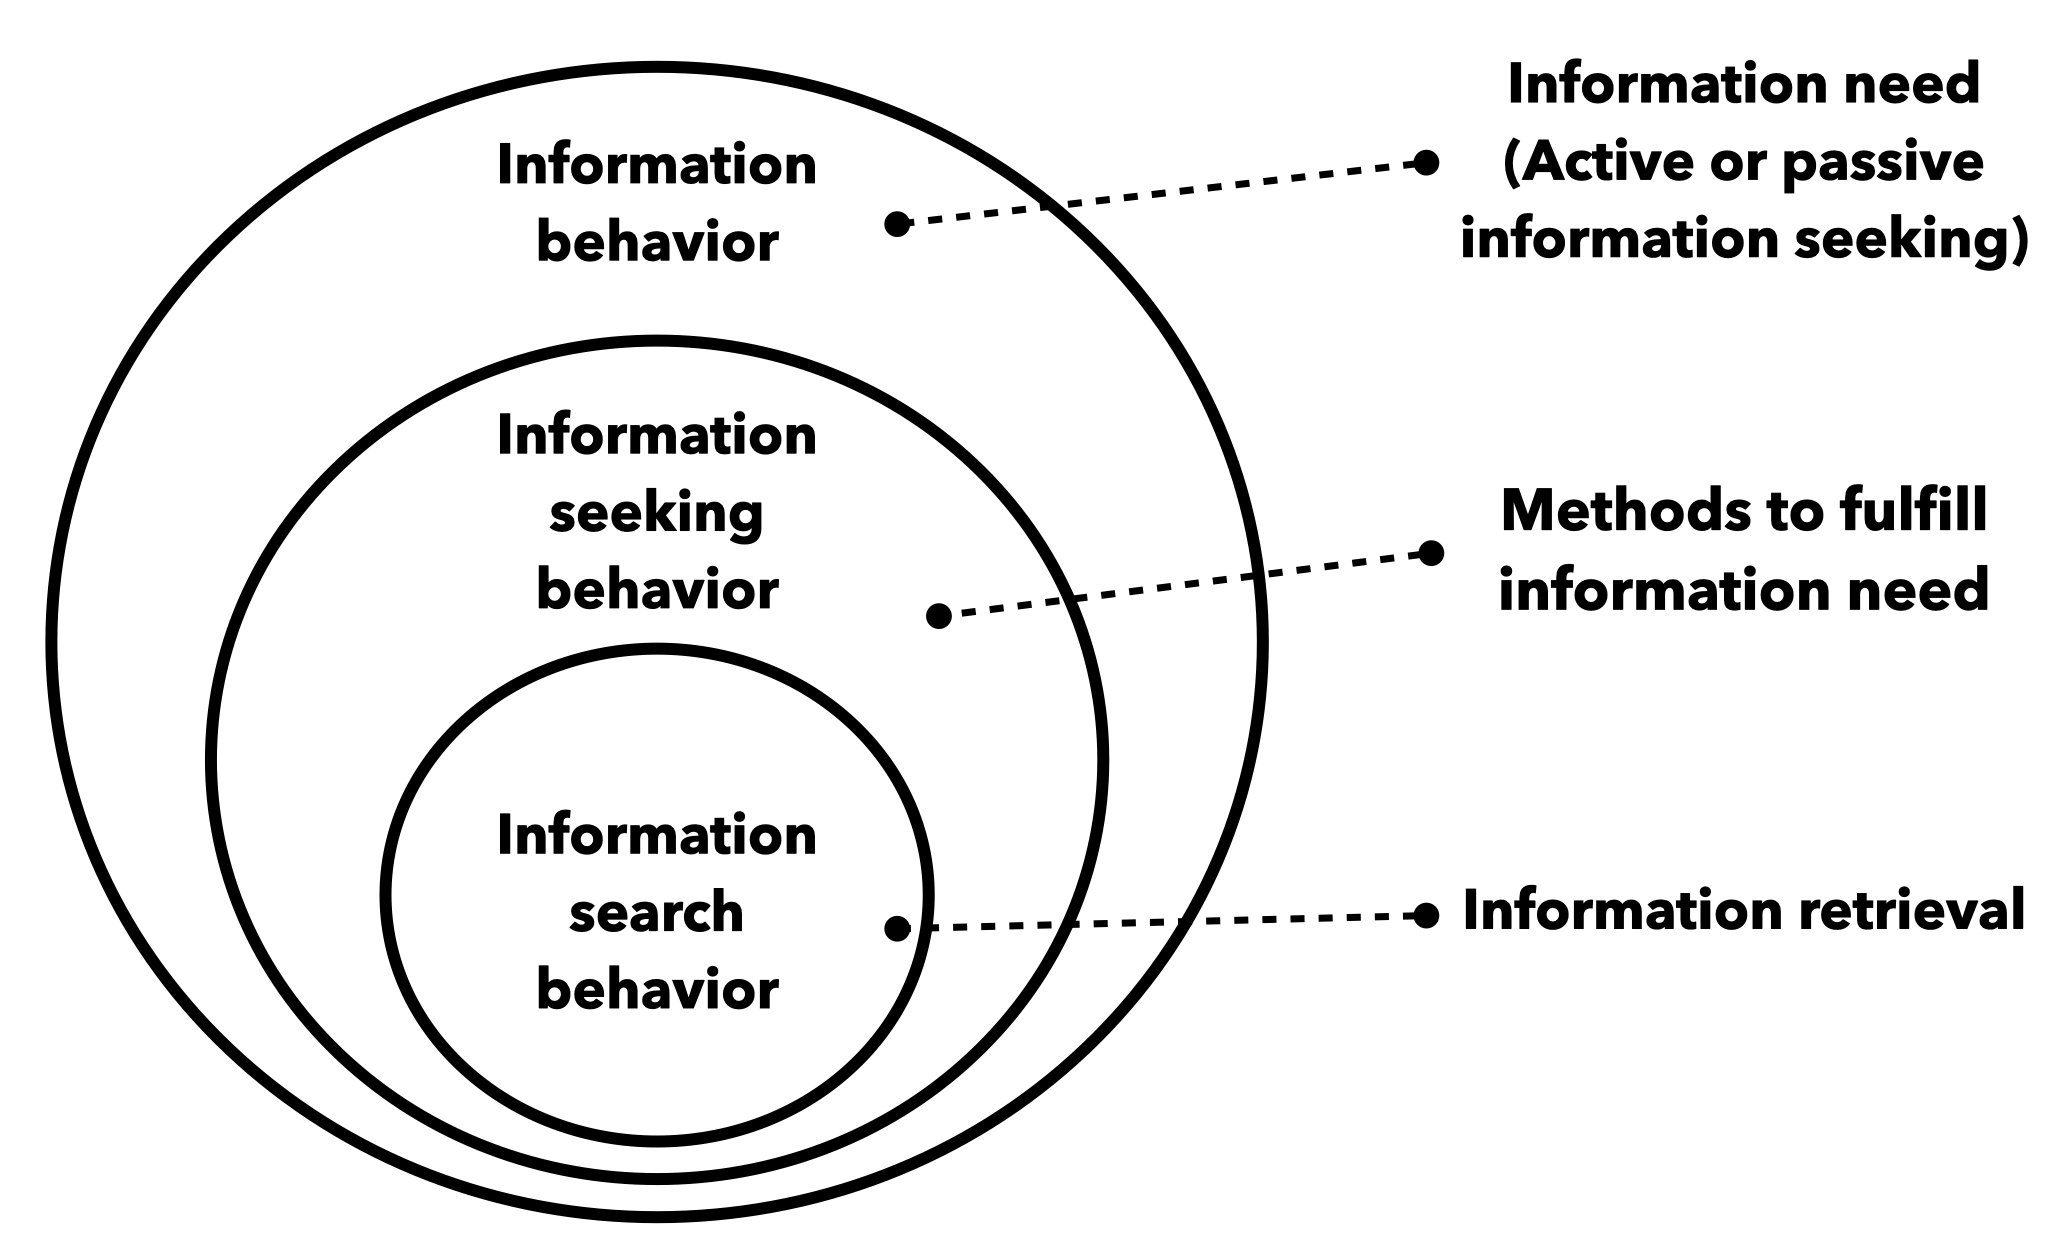
\includegraphics[width=.6\textwidth]{images/thesis_images/information_behaviors.png}
	\caption{Nested model of information behavior~\cite{informationrModelsInformation}. \label{fig:information_behaviors}}
\end{figure} 

Irrespective of whether individuals are active or passive information seekers, they need more information and want to seek information from external sources. Due to the lack of information, users interpret the information gap as a problem and try to manage or resolve this problem by interacting with information sources~\cite{belkin1993interaction}. These user activities are characterized as information seeking behaviors~\cite{belkin1993interaction} and are referred as information search behaviors when seeking the information through a search query. \prettyref{fig:information_behaviors} shows the nested relationship between the different information behaviors, as depicted by Wilson~\cite{informationrModelsInformation}. This depiction highlights that information search behavior is a subset of information seeking behavior, which, in turn, is a subset of information behavior.


In this master thesis, we consider the behaviors related to text interacting information seeking. Furthermore, the thesis is explicitly targeted toward specific and exploratory information-seeking behaviors to understand and help the users in their information-seeking process effectively.

\section{Motivation}

Irrespective of the search platform, the quality of the search results relies on how well the information seekers formulate their information needs. This principle is often referred to by researchers as the "Quality-in quality-out" principle: \textit{A query that more accurately reflects the user's information need will produce better results}~\cite{croft1987i3r}. Consequently, the formulation of the query plays a critical role in the information seeking process. However, assessing the quality of a formulated query can be challenging and is influenced by various factors, including the user's knowledge of their information need, prior search experience, system experience (user interface), and more~\cite{marchionini2007find}.

 \ac{QC} is a widely adopted technique that assists users in formulating their information needs more effectively. \ac{QC} capitalizes on actively indexed data available on the web and leverages query logs generated by millions of users. This technique is commonly observed in modern browsers, offering features such as real-time auto-completion and spelling correction~\cite{bast2006type, gaizauskas1998information}. Studies by Marchionini and White~\cite{marchionini2007find} indicate that information seekers show better engagement in their search activities when using \ac{QC}, resulting in higher levels of user satisfaction. However, even after the query is successfully formulated using \ac{QC}, there are some possible reasons for poor search results (low relevancy)~\cite{azad2019query}. 

\begin{description}
	\item[Cross-domain queries] \hfill \\ These are user queries that span multiple domains or topics, leading to an abundance of false positives. The resolution lies in constructing a well-defined query that aligns with a specific topic based on the information seeker's interest.
	
	\item[Short queries] \hfill \\ When the query length is too short, then the user's information need is not well expressed. A recent analysis to understand the user search queries on 306 million keywords used in google search showed that user queries were comprised of a relatively small number of keywords and the mean keyword length is 1.9 words and 8.5 characters~\cite{google_keyword}. \prettyref{fig:longtail_keywords} provides further insights by examining the distribution of search queries based on their length. It is evident that shorter user queries, indicating weaker intent, are more prevalent compared to longer queries with stronger intent. This pattern namely "Long tail" search queries show the significance of short keyword queries within the user search behavior.
	
	\begin{figure}[h]
		\centering
		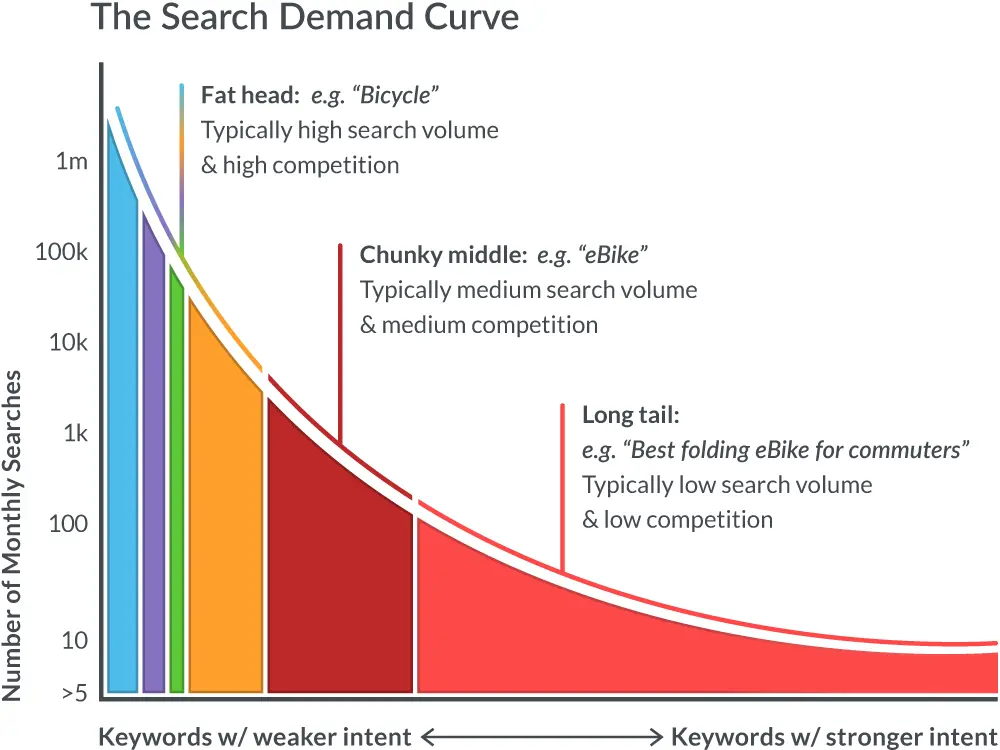
\includegraphics[width=.55\textwidth]{images/outside/search_demand_curve.png}
		\caption[Search query distribution]{Distribution of search queries according to their length~\cite{mozWhatKeywords}. \label{fig:longtail_keywords}}
	\end{figure} 
	
	\item[Poor information needs] \hfill \\ The user is only sure what they are looking for once they see the search results. The user should conduct an exploratory search on a topic and learn from the results.
	
	\item[Poor query formulation] \hfill \\ In this case, users have a clear understanding of what they want to search but struggle to appropriately formulate the search query.
\end{description}

The length of documents in the information source can significantly impact search results. Smaller text documents commonly found in \ac{NLP} projects, such as IMDB reviews and tweets, are typically associated with a single class or topic. Conversely, longer documents like news articles, blogs, e-books, and research papers often contain multiple topics and cannot be logically mapped to a single topic. When such lengthy documents appear frequently in search results, it can result in poor user satisfaction due to their low relevancy (due to the above-mentioned reasons).


To address this issue, users should create well-defined queries that clearly express their intent. For example, a query such as "What are the technological advancements in Robotics related to Unmanned Weapon Systems?" demonstrates a well-formulated query specifying the desired information. However, demanding users to consistently provide such specific queries can be challenging, particularly in exploratory tasks where users may be uncertain about what they are searching for. Additionally, this approach may lead to a sub-optimal search experience, as it restricts users to only certain types of queries.

Rather than expecting users to consistently formulate precise queries, an alternative approach is to guide them using interactive relevance paths derived from a simple user query. These relevance paths are representations of documents extracted from the top retrieved documents for the original query. This methodology is rooted in the concept of "Content-driven information seeking"~\cite{marchionini2007find}, which assumes that the top documents are relevant to the query. Research findings suggest that content-driven relevance paths offer benefits for both exploratory searches and known-item searches~\cite{marchionini2007find}. Particularly when dealing with long text documents, these content-driven interfaces can assist users in narrowing down the search space and finding relevant documents more efficiently. To help users with highly heterogeneous topics within search results, this master thesis proposes an effective and unsupervised topic extraction technique from the top search results.
 
\section{Research Questions}

\ac{IE} and \ac{IR} are two highly effective techniques used in research to fulfill user information needs. \ac{IE} refers to the automated extraction or mining of specific information from data, while IR focuses on retrieving relevant documents for a given user query. Gaizauskas and Wilks~\cite{gaizauskas1998information} have emphasized the complementary nature of these techniques and highlighted the potential for creating practical and robust tools by combining them. For instance, \ac{IE} can aid in formulating the user's information need more accurately, while IR can facilitate the retrieval of high-quality search results.
 
This master thesis introduces an interactive system that integrates both \ac{IE} and \ac{IR} techniques to effectively meet user information needs. The thesis presents an unsupervised soft clustering approach designed to model documents in multiple languages as a mixture of sub-topics. These sub-topics are extracted using deep intrinsic information derived from keywords. The evaluation of this approach is conducted in three phases, including not only the assessment of clustering using various evaluation metrics but also a user satisfaction survey. The research questions (RQ) detailed below specifically address the evaluation of the proposed approach.

\begin{enumerate}
\item[RQ1:] How effective is the sub-topic modeling approach in creating distinctive clusters from long text documents?

Clustering algorithms generate topics (well-formed clusters) from a collection of documents. However, these topics become highly valuable to users when they exhibit distinctiveness especially in the case of news-articles. The presence of heterogeneous clusters enables users to easily identify relevant documents related to both the query and the sub-topic cluster. To generate such highly distinctive clusters, a candidate keyword selection approach is introduced and evaluated. This research question aims to assess the effectiveness of the keyword selection technique when combined with conventional clustering. Both intrinsic and extrinsic clustering evaluation techniques and a survey are chosen to evaluate the clustering output. The parameters of the clustering pipeline are fine-tuned using these evaluation metrics and manual observation.



\item[RQ2:] How can the retrieved documents be effectively represented for a given user query and sub-topic?  \\

When users select a specific sub-topic cluster, it is assumed that the retrieval results relevant to both the user query and the chosen sub-topic are presented to the user. In this master thesis, two distinct  \ac{IR} systems are proposed to retrieve documents relevant to the user query and the selected sub-topic. The objective of this research question is to compare these two \ac{IR} systems and determine the better system. A survey is performed, and the collected data is analyzed to answer the RQ2. Survey participants have the opportunity to read the retrieved documents from both \ac{IR} systems and respond to five questions. A statistical test is performed on the survey data to determine whether the results from the two \ac{IR} systems exhibit any significant differences. Further details regarding the  \ac{IR} systems and survey questions are provided in subsequent sections of the report.


\item[RQ3:] What is the impact of sub-topic and document rankings on the identification of positive documents from the candidate pool? \\

Displaying only documents related to a specific sub-topic can restrict users from accessing all relevant retrieved results for a given query. This research question addresses the impact of the sub-topic clustering output to find the positive documents against the baseline approach. An exploratory precision analysis is conducted to evaluate this impact. Additionally, this research question aims to extract valuable insights from the clusters and their rankings. For instance, \textit{Does a particular sub-topic cluster ranking yield higher precision compared to the baseline?} To address this research question, the widely used \ac{IR} evaluation metric, \ac{MAP}, is used for ranking analysis. Furthermore, the proposed approach's retrieval performance is compared to the literature.

\end{enumerate}


\section{Thesis Structure}

This master thesis is structured into seven chapters, spanning from Chapter 2 to Chapter 8. Chapter 2 delves into the problem context, emphasizing the problem statement. In Chapter 3, essential technical information and background are provided to facilitate comprehension of the selected technologies used in implementing the proposed methodology. Following that, Chapter 4 comprehensively examines the relevant literature that relates specifically to the master thesis. Chapter 5 outlines the proposed approach in detail. Subsequently, Chapter 6 illustrates the experiment setup, while Chapter 7 presents the experiment results. Finally, in Chapter 8, critical aspects of the thesis are highlighted, including an overview of the limitations and suggestions for future work.




    
         % !TEX root = ../thesis.tex

\chapter{Problem Context}

In this chapter, the problem addressed in this master thesis is introduced, and an overview of the existing work is provided. The first section "FKIE" presents the scope of the problem and outlines the expectations of the \ac{IR} system from target users perspective. Subsequently, the definitions of several crucial keywords and technologies are provided in the section "Key Definitions". Additionally, the previous work conducted prior to this master thesis is discussed in the section named "Existing Work". Finally, "Problem Description" delves into the challenge in detail with presenting statistical information and discussing the potential of addressing the problem using well-established techniques.

	\section{FKIE}

The \ac{FKIE} is a renowned research institute dedicated to pioneering solutions in information and communications technology. Their primary focus lies in the development of effective and efficient human-machine systems\footnote{\url{https://www.fkie.fraunhofer.de/en/about-fkie.html}}. The users at \ac{FKIE} have a particular interest in accessing news articles that are related to  innovation and advancements in the fields of technology and military. \prettyref{fig:areas_of_interest} provides a visual representation of the areas of interest to the \ac{FKIE} users. It is important to note that this list is not bounded and can encompass additional domains.

\begin{figure}[h]
	\centering
	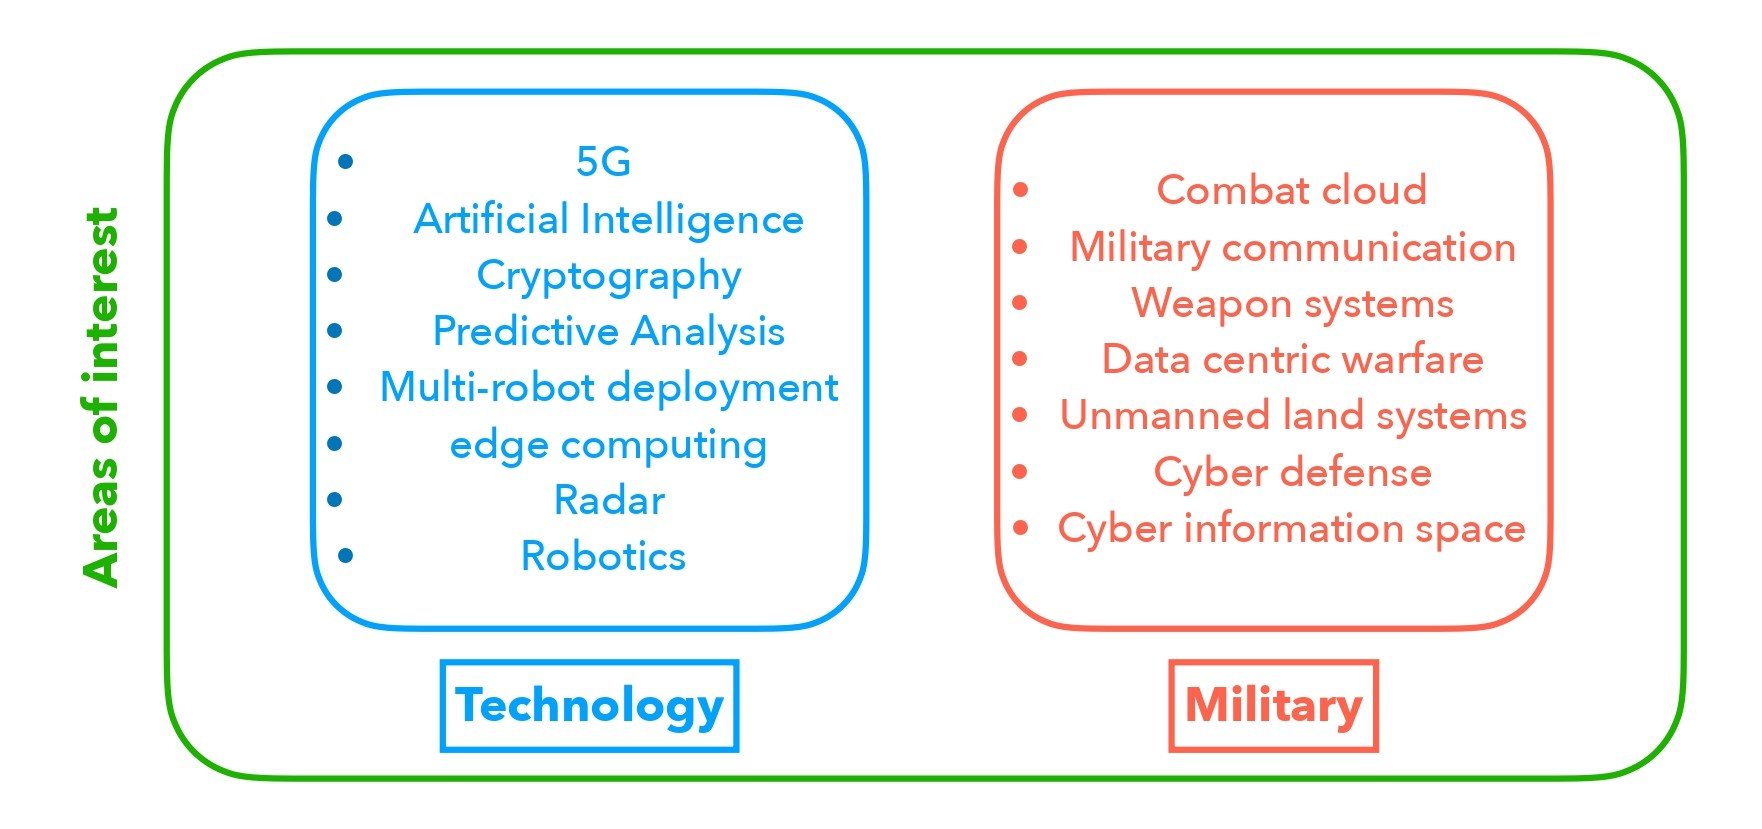
\includegraphics[width=.8\textwidth]{images/keynotes_images/areas_of_interest.jpg}
	\caption{Areas of interest for users at FKIE. \label{fig:areas_of_interest}}
\end{figure} 

\section{Key Definitions}

This section provides explanations of several key technologies utilized in the previous work and additional definitions can be found in Appendix A.

\begin{description}
	
	\item[\ac{SVM}] \hfill \\ The \ac{SVM} is a supervised learning algorithm commonly utilized for classification and regression tasks. It operates by selecting a maximum margin separating hyperplane (also known as a decision boundary) based on the labeled data information. This hyperplane is then used to classify new data points~\cite{noble2006support}.
	
	\item[Lexical matching] \hfill \\ Lexical or syntactic matching is a technique that calculates a relevance score between two text data (strings) by considering the terms present in the data. However, this matching technique is sub-optimal for retrieval purposes since it does not take into account the semantic meaning of the query~\cite{kuzi2020leveraging}.
	
	\item[BM-25] \hfill \\ BM-25, also known as Best Match 25, is a ranking function derived from a probabilistic relevance framework. It assigns ranks to documents based on the occurrence of query terms within each document~\cite{amati_bm25_2009}. However, it should be noted that BM-25 ranking operates on a lexical or syntactic matching approach and does not take into account the semantic meaning of the words.
	
	\item[Semantic search] \hfill \\ Unlike syntactic matching or simple term frequency calculations, semantic search engines aim to understand the underlying meaning of a search query. They strive to retrieve documents that are closely related to the query in the semantic space, taking into account the contextual understanding of the query~\cite{dong2008survey}.
	
	\item[Document index] \hfill \\ Document indexing or compression is a technique that enables the storage of documents in an optimized manner to enhance retrieval efficiency. The stored data that enables efficient retrieval is commonly known as a document Index~\cite{ziviani2000compression}.
	
	\item[Inverted index] \hfill \\ Inverted index is a data structure that captures every unique word present in the corpus along with a separate list of documents where each word occurs~\cite{ziviani2000compression}. This indexing technique provides efficient real-time retrieval of documents.
	
	\item[Elasticsearch] \hfill \\ Elasticsearch\footnote{\url{https://www.elastic.co/what-is/elasticsearch}} is a search engine that is specifically designed for handling textual data. It serves as both a document index and a retrieval system for user queries and uses lexical matching techniques. Elasticsearch leverages the inverted index data structure for efficient storage of documents and enables rapid full-text searches.
	
	\item[Semantic search index] \hfill \\ Semantic search index, also known as a vector database, is responsible for storing distributed embedding vectors of the documents. These vectors are utilized during the retrieval process to enable semantic search.
	
	\item[FAISS] \hfill \\ \ac{FAISS}, a library specifically designed for efficient similarity search and it is employed in this thesis to store document embeddings. The semantic search system developed in this research uses \ac{FAISS}. As a ranking function, \ac{FAISS} utilizes L2 euclidean distance to measure the similarity between the query and documents~\cite{githubGitHubFacebookresearchfaiss}. In this thesis, the output of this distance function is further refined by re-ordering it based on cosine similarities.
	
	\item[News article] \hfill \\ A news article, which is considered a text document, is typically published by a news website. \prettyref{fig:sample_newsarticle} provides an example of a news article. In this master thesis, the terms 'news article' and 'text document' are used interchangeably to refer to the same concept.
	
	\begin{figure}[h]
		\centering
		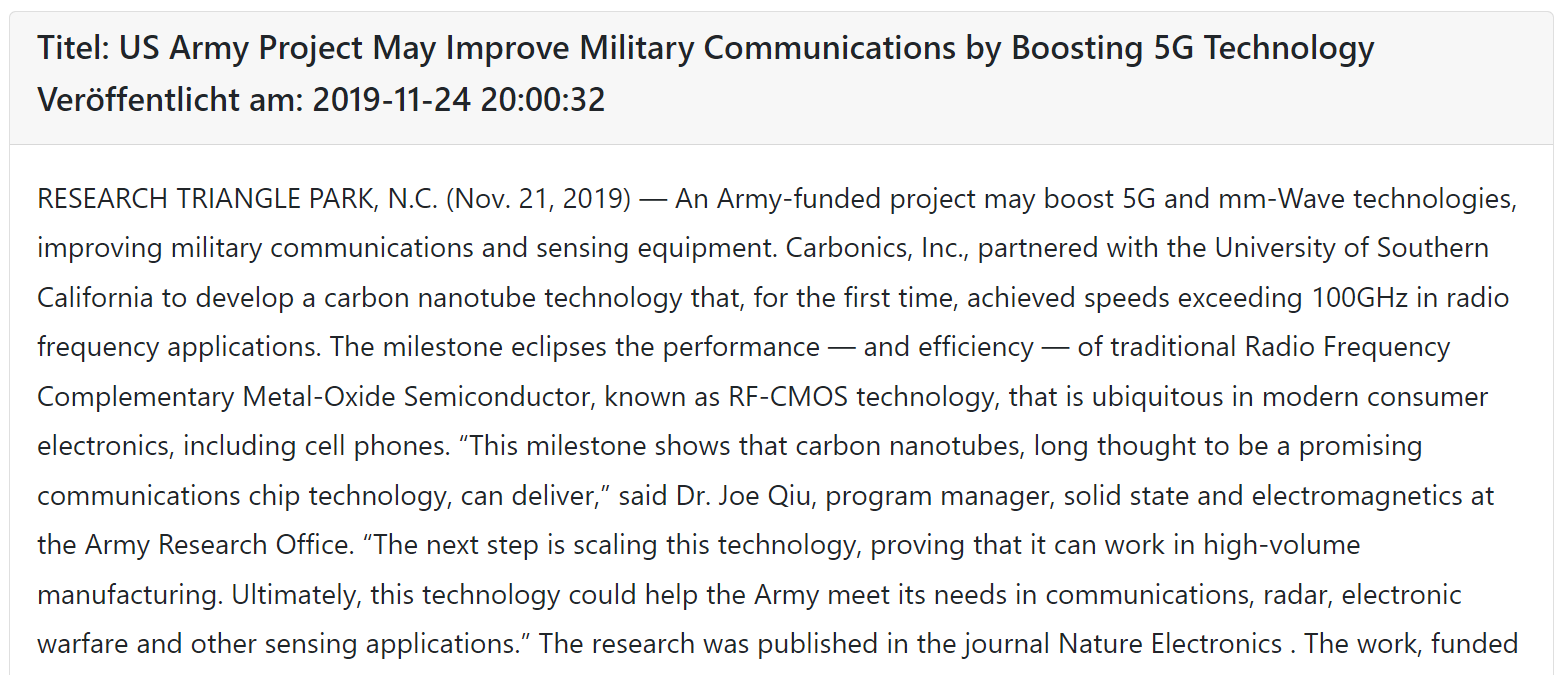
\includegraphics[width=.8\textwidth]{images/mitera_screenshots/sample_news_article.PNG}
		\caption[News article example.]{A sample news article from the document database~\cite{sample_news_article}.\label{fig:sample_newsarticle}}
	\end{figure} 
	
	\item[Web scraping] \hfill \\ Web scraping refers to the automated extraction of data from websites~\cite{khder2021web}. When dealing with text data, various approaches involve downloading structured HTML webpages and extracting the required information. In this master thesis, news articles from different websites are scraped using the framework Scrapy\footnote{\url{https://scrapy.org/}}.  
	
	\item[Candidate pool] \hfill \\ The candidate or retrieval pool refers to a collection of documents obtained from lexical and semantic matching results for a specific user query. These documents show diversity and often contain keywords that are present in the query or have semantic similarity to them. The retrieval pool serves as a basis for subsequent clustering analysis.
	
	\item[Sub-topic] \hfill \\ Sub-topics are intermediate representations of a document that provide more granular information. Since news articles are typically lengthy texts and cannot be logically associated with a single topic or keyword. Therefore, sub-topics are derived to capture distinct aspects within them. In the context of the "Retriever", if the user query is regarded as the main topic, the sub-topics correspond to the distinctive topics extracted from the candidate pool. In this master thesis, the terms "sub-topic" and "cluster" are used interchangeably. 
	
	\item[Query type] \hfill \\ The user's search queries can take various forms and in this master thesis, each specific form is referred to as a query type. All possible user queries can be categorized into two major query types: phrase (three words or less) and sentence queries.
	
\end{description}

\section{Existing Work}

A document retrieval system was developed to assist users at \ac{FKIE} in accessing news articles related to technology and military subjects. The retrieval system comprises three main components: the "Web scraper", the "Document filter", and the "Retriever", as illustrated in \prettyref{fig:background_image}.

\begin{figure}[h]
	\centering
	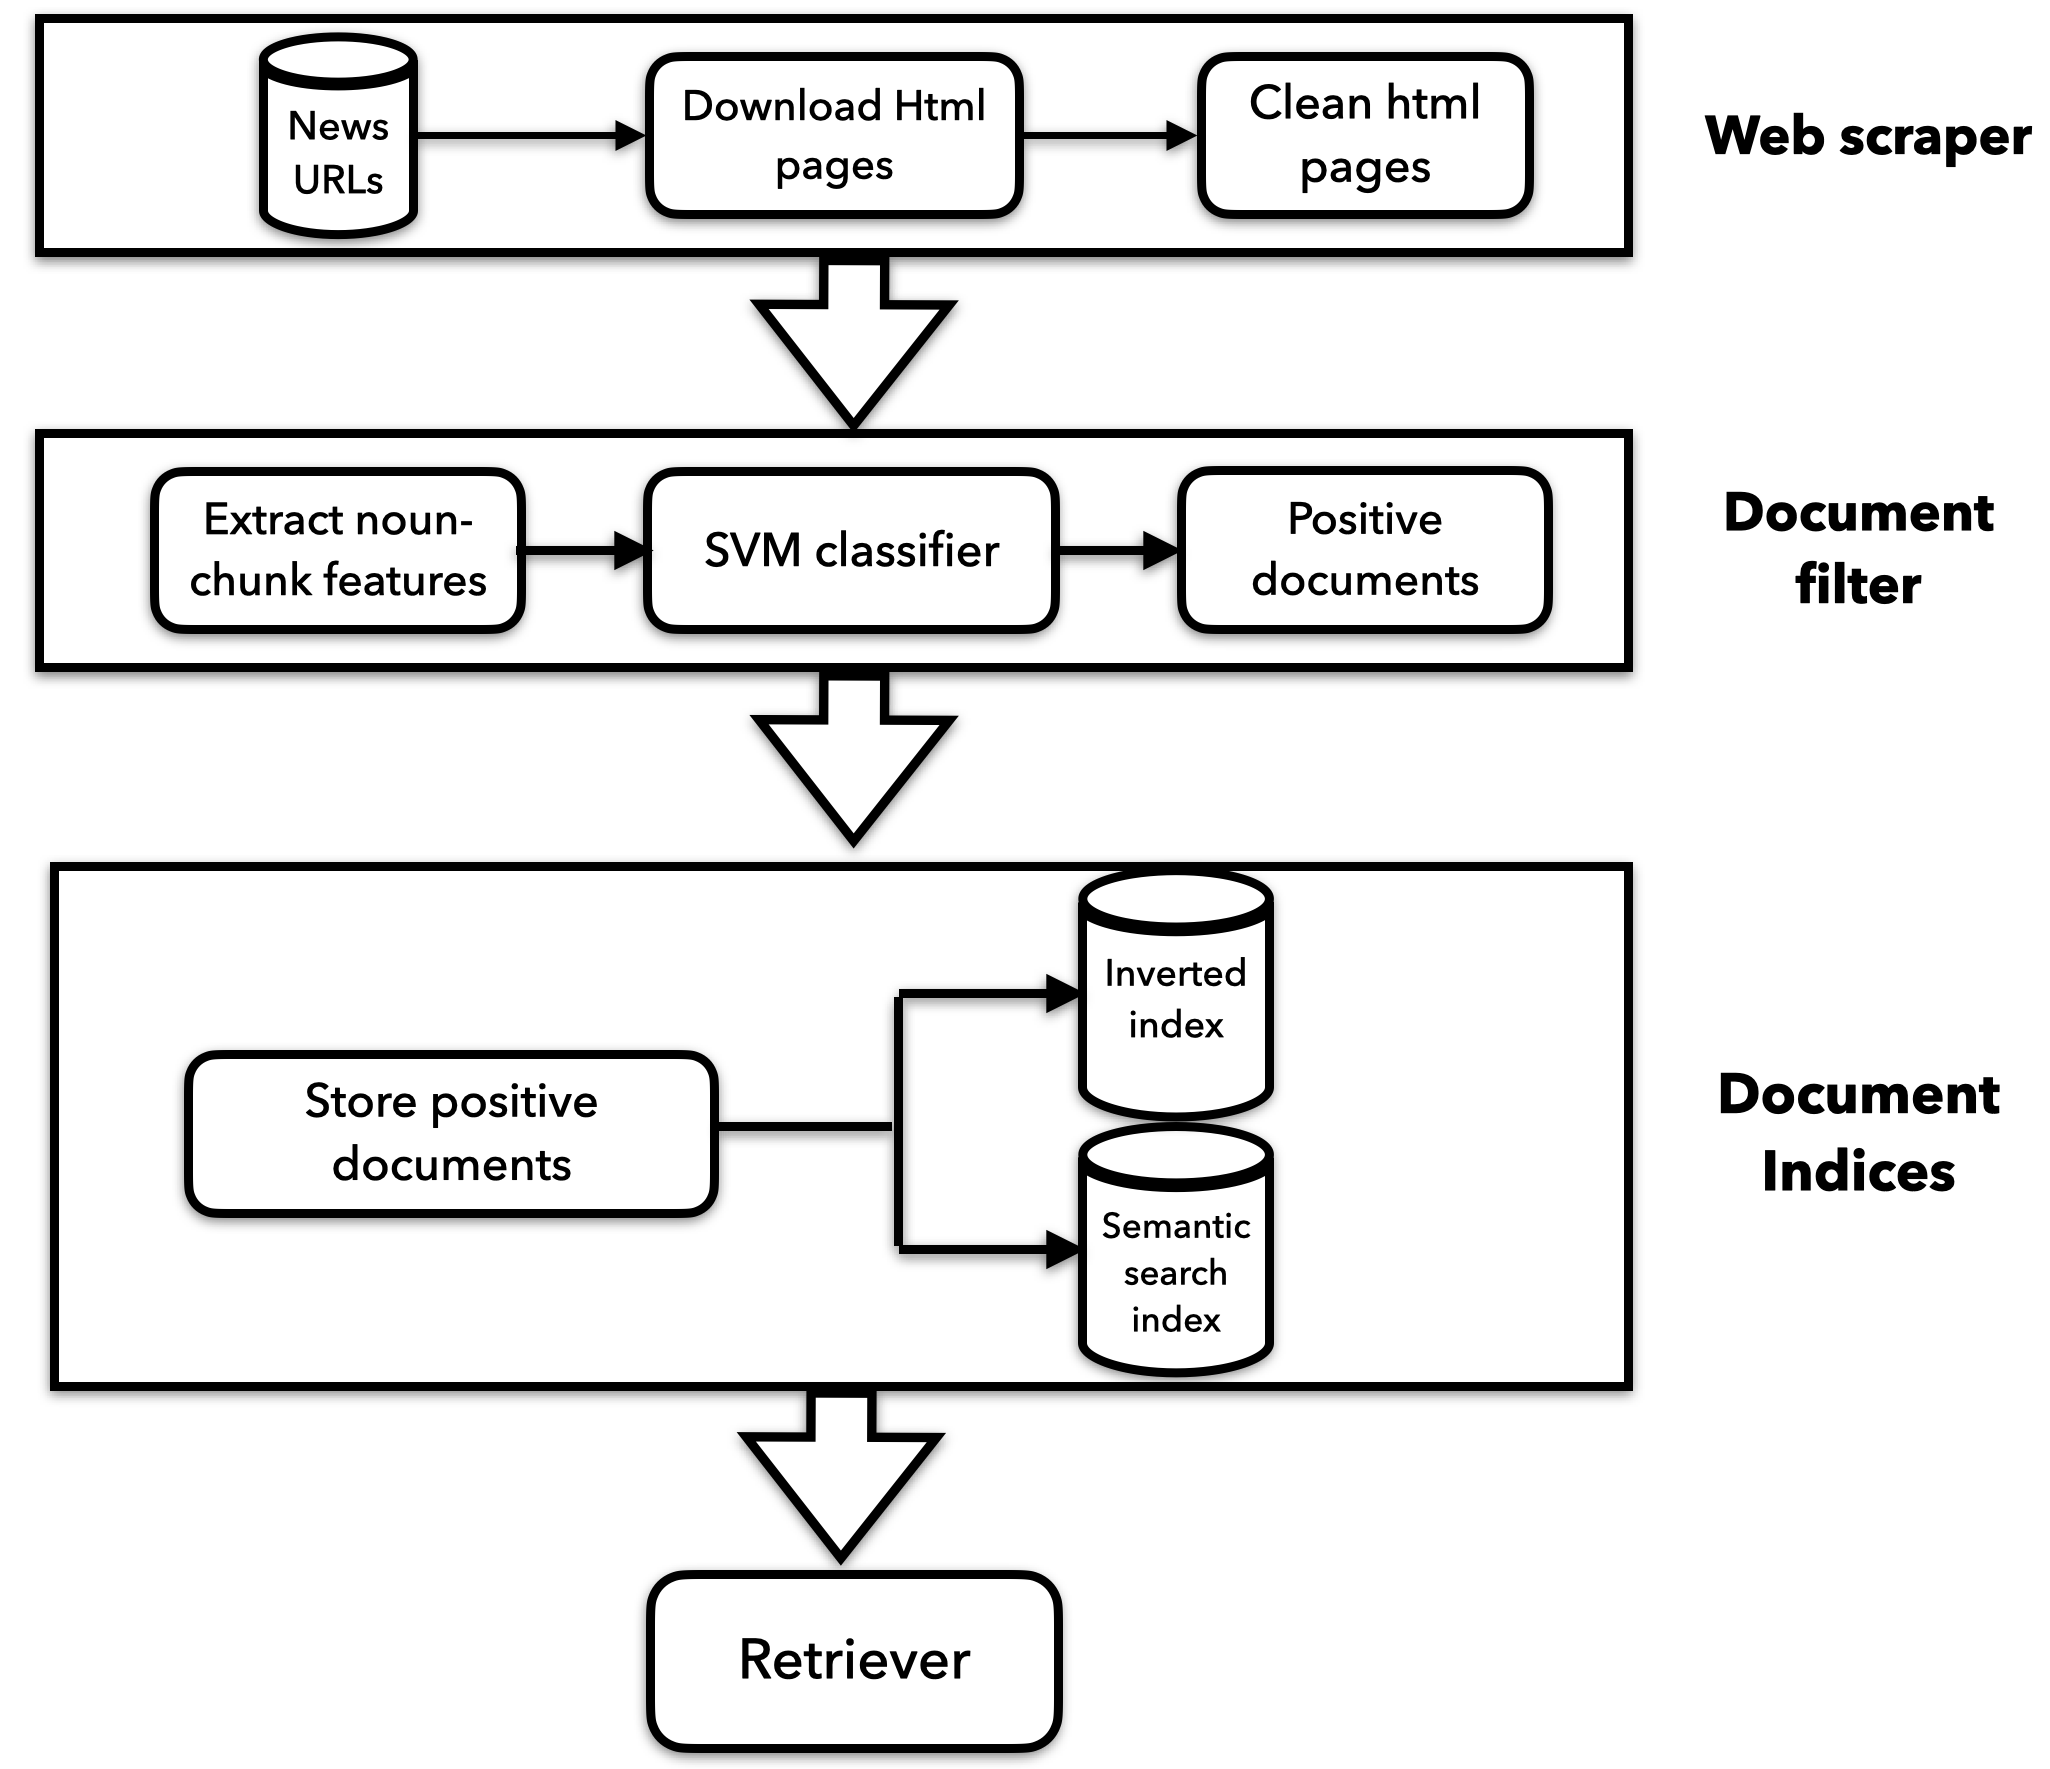
\includegraphics[width=.9\textwidth]{images/thesis_images/background.png}
	\caption[Existing work developed at FKIE.]{Document retrieval system designed at FKIE. \label{fig:background_image}}
\end{figure}

The first component, known as the "Web scraper", retrieves news articles in the form of HTML files from a predefined list of URLs. It then proceeds to clean the raw HTML data by removing advertisements and other irrelevant content. Each cleaned news article is treated as an individual entity referred to as a "Document". The majority of downloaded documents cover a range of topics including military, technology, artificial intelligence, and other typical news subjects like politics, sports, and advertisements. These news articles are available in both German and English.

The second component, referred to as the "Document filter", employs a \ac{SVM} classifier to filter out irrelevant documents that are not related to specific news topics. The documents are classified into two distinct classes: "Positive" and "Negative". Positive documents are news-articles related to technology and military topics, while the negative documents cover all other subjects. Various features from different techniques, such as noun-chunks, verbs, adjectives, and fine-tuning of \ac{BERT} models, have been evaluated. The results indicate that features derived from noun-chunks in a document yield the best performance in distinguishing between positive and negative documents. Noun-chunk features based on the pre-trained multi-lingual \ac{USE} are utilized for the classification task.

\begin{figure}[h]
	\centering
	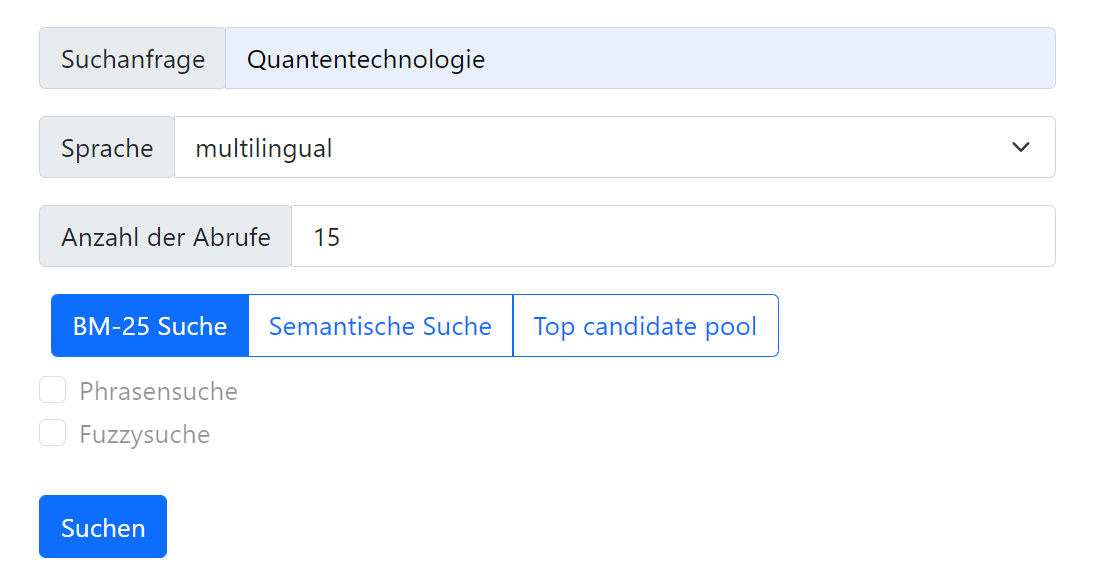
\includegraphics[width=.7\textwidth]{images/mitera_screenshots/newsfeeds_search.PNG}
	\caption[Search user interface.]{User interface to retrieve documents for FKIE users. \label{fig:mitera_search}}
\end{figure}

The positive documents obtained from the "Document filter" stage are stored in two separate document indices, namely the inverted index and the semantic search index (see definitions above and Appendix A for more details). To retrieve documents for a given user query, a dedicated "Retriever" component has been developed, which utilizes both indices and employs lexical and semantic matching techniques. The retrieval process is assisted through a user-friendly web interface, as depicted in \prettyref{fig:mitera_search}. A total of 327,421 news articles were initially scraped, and after applying the document filtering, 26,954 news articles were stored in the document indices. These stored documents are further used in the retrieval process.


\section{Problem Description}

Semantic matching is particularly effective when dealing with long sentence queries due to the contextual information embedded in the search query. For example, a detailed query such as \textit{What are the technological advancements in Robotics related to Unmanned Weapon Systems?} yields high-quality results in the top search results, as it provides specific and comprehensive information requirements. However, in case of keyword queries, semantic and lexical matching approaches tend to generate numerous false positives and offer no significant advantages. This issue of false positives and lack of uniqueness in lexical matching was also observed by Kuzi et al.~\cite{kuzi2020leveraging} in their research.


 Lexical matching does not consider the inherent meaning of the word causing a vocabulary mismatch problem especially in case of polysemy, synonymy. For example, the words "Vehicle," "Automobile," and "Car" essentially refer to the same thing, but lexical matching techniques fail to establish their relationship. Conversely, semantic matching may retrieve a large number of documents that match the query keywords semantically, but it often fails to present the most relevant documents in the top search results. A manual observation of retrieved results is carried out with a set of sample queries to evaluate the retrieval algorithms,and the results are shared in \prettyref{tab:ir_system_comparison}.


\begin{center}
	\captionof{table}[Retrieval algorithms comparison.]{Retrieval algorithms comparison on different query types.}\label{tab:ir_system_comparison}
	\begin{tabularx}{.99\textwidth}{|c|Y|Y|Y|Y|}
		
		\hline
		S. No. &  Query type & Better retrieval technique &  Reason &  Queries used  \\
		\hline
		1 & No meaning queries & BM-25 &  Lexical matching  & Person or object names\footnote{User query with no innate meaning of the word namely out of vocabulary words: for example John Dowe, Wester etc.} \\
		\hline
		2 & Multi-lingual queries & Semantic search &  Semantic matching & Artificial Intelligence vs Künstliche Intelligenz\\
		\hline
		3 & German composite words  & Semantic search&  Semantic matching & Quantentech- nologie \\
		\hline
		4 & Spelling mistakes  &  Semantic search&  Semantic matching & Kryptografy, Rbot \\
		\hline
		5 & Polysemy  & Semantic search&  Semantic matching & Combat Cloud, Cloud computing \\
		\hline
		6 & Sentence/long phrase queries  & Semantic search&  Semantic matching  & Schwachstell-
		enanalyse eigene Waffen-Systeme \\
		\hline
		
	\end{tabularx}
\end{center}

The users at \ac{FKIE} typically provide concise phrase queries which usually consists of just one or two words. Their intention is to explore information related to specific topics such as "Technology" and "Military". However, learning the user's intention solely based on a single word or phrase query poses a significant challenge in the absence of labeled data. Additionally, another obstacle arises from the diverse range of information sources, which can result in high levels of noise and an increased likelihood of encountering false positives. As a consequence, users are less likely to find the relevant documents among the top search results. 


\begin{figure}[h]
	\centering
	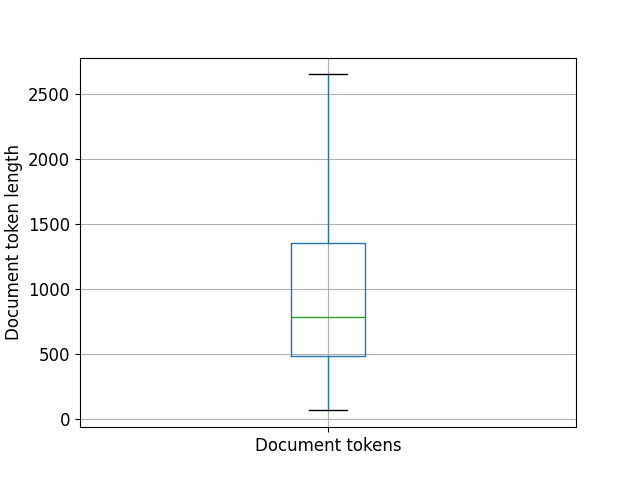
\includegraphics[width=.65\textwidth]{images/keynotes_images/token_length_boxplot.png}
	\caption[Document length distribution.]{Document token length distribution (after removing the outliers). \label{fig:token_length_distribution}}
\end{figure}

Unlike tweets or abstract natural language requirements, news articles are lengthy text documents with a median token length of 788 and encompass keywords from multiple domains. The distribution of document token lengths is illustrated in \prettyref{fig:token_length_distribution}. Finding information regarding innovation and technological breakthroughs within news articles poses a significant challenge. Information related to innovation and technological breakthroughs is hard to find in the news-articles. However, the probability is not zero, as positive news articles are gathered during data collection for classification. Due to these challenges, achieving a supervised solution that can match the performance of a full sentence query is challenging. Real-time user feedback and continuous reinforcement algorithms have the potential to address the lack of labeled datasets. However, they require regular feedback from diverse users to avoid biased results that favor a particular user.



\begin{center}
	\captionof{table}[Clustering results in German and English.]{Clustering results to generate more document representations in German and English.}\label{tab:clustering_100_output}
	\begin{tabularx}{.99\textwidth}{|c|Y|}
		\hline
		Query & Clusters \\
		\hline
		
		Quantentechnologie     & Technologie, Microsoft, Military, KI, Quantenteilchen, Quantum computing, Forschung, Bundesministerium, Quantencomputer, München, Industrie, Netzwerke, Algorithm, Quantencomputing, Ingenieuren Informatiker, Qubit, Programmierung, Marineschiff, Intelligence, China, Verteidigung, IBM, AI, Quantum physic, Wissenschaftler, Electronic, Prozessor, Deutschland, Future, Vorsprung, Robotic, Compute, Memory SSDs, USA, Entwicklung, Raumfahrt, Klima, Cybersicherheit, Stau, Rheinmetall Waffe, Laserstrahl \\  \hline
		
		5G          & 5G, 5G network, Frequenzspektrum, 5G deployment, China, Defence intelligence, Nokia, Berlin, Mobilfunkmast, Telekom, Gigabit speed, 4G, WiFi, UMTS, Military, Fiberoptic broadband, 5G technology, Vodafone, Experimentation testing, Mobilfunknetzbetreiber, Technologie, Netzwerk, LTE, Smartphones, Netz, Aircraft, 5G service, Data cap, Deutsche Telekom, Telefónica, Apple, Gebiet, Netzausbau, Anbieter \\  \hline
		
		
		
	\end{tabularx}
	
\end{center}


One approach to enhance the context of a search query is by utilizing a template-based search query. This involves using a predefined template, such as "Innovations in XXX related to the Military."  When the user provides a query such as "Robotics," the "XXX" in the template is replaced with the user's query, resulting in the final query, "Innovations in Robotics related to Military." This template can be dynamically updated based on the user's interests through the user interface, allowing for customized results without the need for additional training. However, this approach has limitations as it restricts users to a limited set of templates and can be inefficient when adding new templates or updating existing ones.


\mycomment{\begin{center}
		\captionof{table}{Keywords present in one retrieved document for the query Quantentechnologie.}\label{tab:keywords_distinction}
		\begin{tabularx}{.75\textwidth}{|Y|Y|}
			\hline
			Keywords similar to the query & Keywords useful for clustering  \\
			\hline
			
			Quantum Technology \newline technological application \newline quantum system \newline quantum computer \newline quantum communication \newline Quantum application \newline quantum bit \newline Quantum sensing \newline quantum radar \newline quantum physics \newline a quantum computer increase \newline a compute unit  &   Sciences  \newline electronic warfare capability \newline the Defense Science Board \newline nuclear material \newline military \newline encode information \newline military personnel \newline military sensing \newline Military Applications \newline Defense Primer \newline enhanced military capability \newline the National Academy \newline potential military application \newline sea-base nuclear deterrent      \\  \hline
			
			
			
		\end{tabularx}
		
\end{center}

One crucial observation has shown that
some keywords from the documents can be omitted during the clustering to improve the clustering
output by creating diverse clusters and maintaining deep representations.  \prettyref{tab:keywords_distinction} details the keywords similar and dissimilar to the query. This query
similarity can play an essential role in creating unique clusters, and it is evaluated extensively
in this thesis.

}

The documents retrieved for certain queries are organized into clusters based on the terms contained within them, forming pathways to access the retrieved documents. The clustering output shown in \prettyref{tab:clustering_100_output}, demonstrates the selection of parameters to generate more comprehensive representations of the retrieved documents. However, it has been observed that some clusters are repetitive and closely resemble the query resulting in the same set of documents being represented and potentially leading to lower user satisfaction.

\begin{figure}[h]
	\centering
	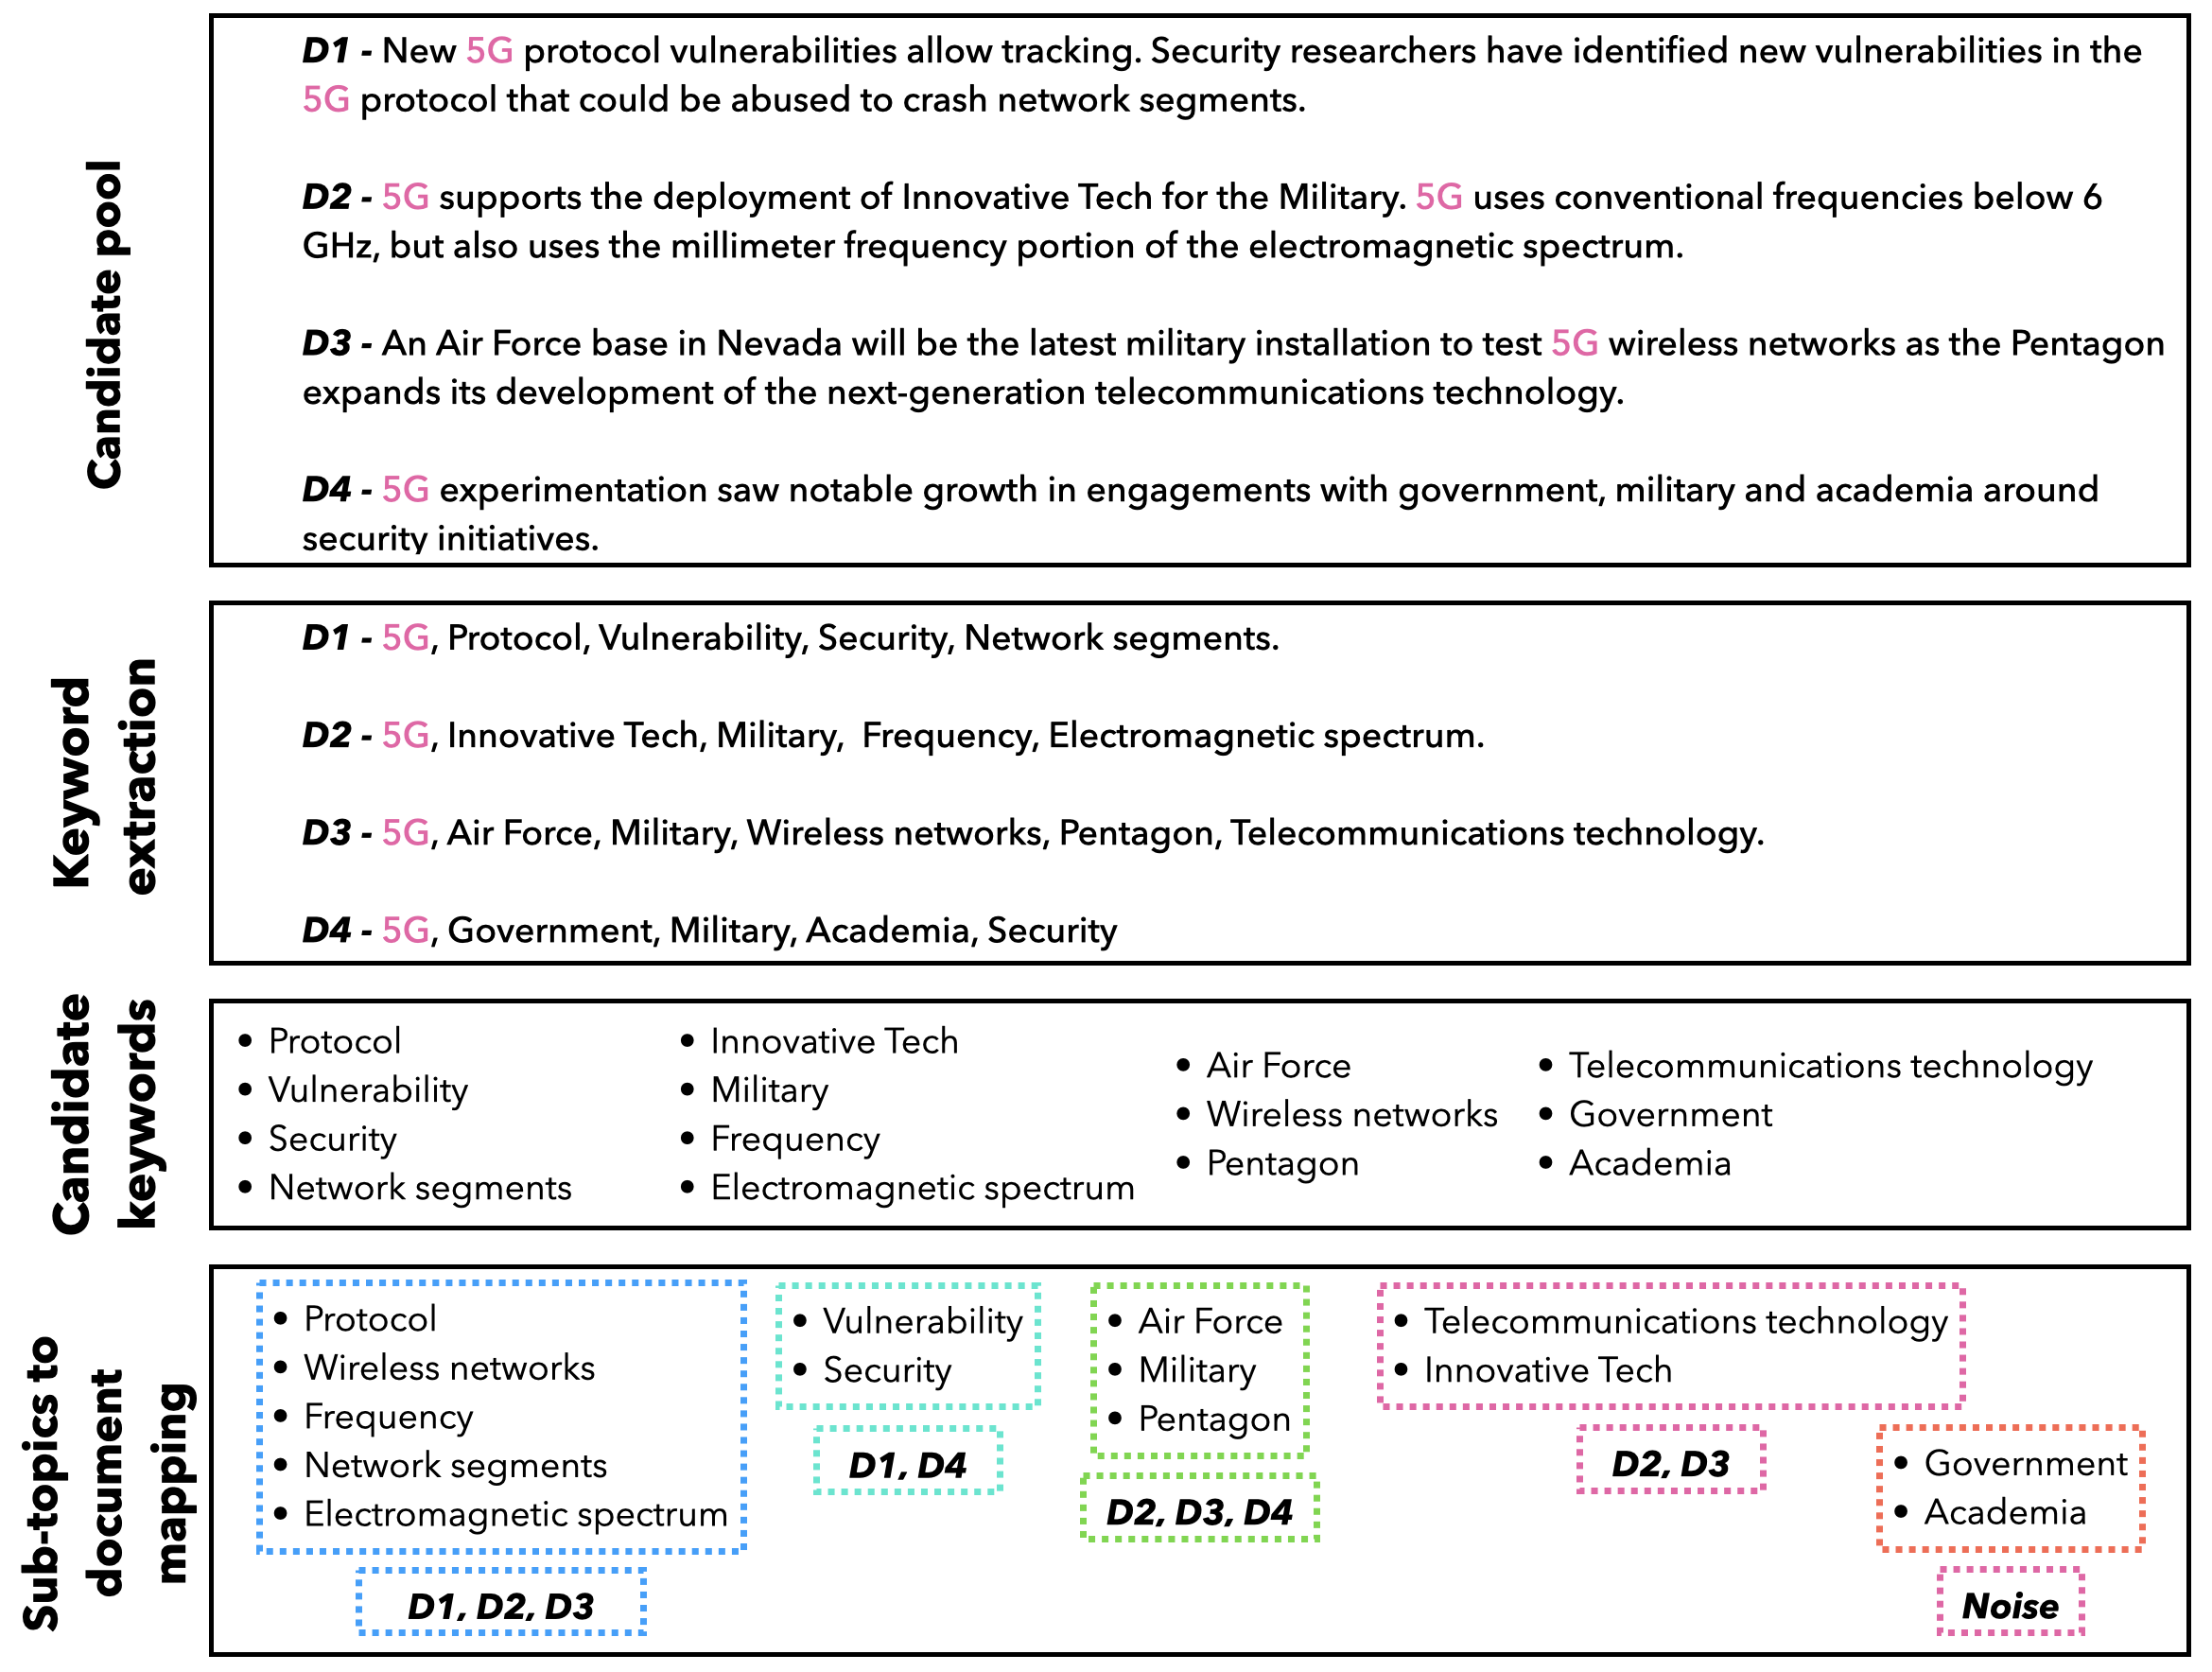
\includegraphics[width=.99\textwidth]{images/keynotes_images/high_level_approach}
	\caption[Expected sub-topic retrieval.]{Expected sub-topic extraction for the query: 5G. \label{fig:proposal_idea}}
\end{figure}

Conversely, selecting parameters that produce fewer representations results in larger individual clusters containing more documents. This, in turn, leads to document repetition within the clusters. After evaluating various approaches to address this issue, we believe that extracting unique contexts in an unsupervised manner from the top results of a user query is more efficient, explainable, and reproducible compared to supervised approaches. This approach not only provides users with deeper insights into the results but also reduces the effort required to find highly relevant documents. 

\prettyref{fig:proposal_idea} presents a sample output of the expected context extraction pipeline, where the extracted unique contexts are referred to as "sub-topics". The proposed approach in this master thesis aims to tackle the aforementioned challenges and generate highly diverse sub-topics. It considers news articles from diverse sources and can be easily adapted to other sources containing long text documents.




       
        % !TEX root = ../thesis.tex

\chapter{Background}

The proposed approach in this master thesis requires a comprehensive understanding of relevant literature related to document representations, ranking architectures, keyword extraction techniques, and other related areas. This chapter provides a thorough technical background for each component employed in the proposed approach. The chapter is organized into six sections, with each section focusing on the literature associated with a specific technology. In these sections, the most suitable techniques selected for the master thesis are discussed in detail.

\section{Sentence Encoders}
In many \ac{NLP} techniques, text documents are commonly represented using distributed vectors. These vectors are constructed based on word or phrase-level representations and play a vital role in various tasks such as exploratory analysis, text classification, clustering, and text retrieval. Besides phrases, incorporating additional meta-information from parts-of-speech and named entities can further enhance the performance of these tasks. Over the past decade, significant advancements in phrase representations have greatly influenced \ac{NLP} research. This section provides a comprehensive review of different phrase representations documented in the literature, with a focus on highlighting the specific representations used in this master thesis.

\subsection{Document Representations from Word Embeddings}

Word embeddings are vectorized representations of words or phrases. For instance, let's consider a text corpus $C$ consisting of $N$ documents, and the vocabulary size is denoted as $M$. In this context, each document is represented as $D$, and individual terms are represented as $t$.

\centerline{$C$ = $\{D_1, D_2, D_3,\dots, D_N\}$ }
\centerline{$V$ = $\{t_1, t_2, t_3,\dots, t_M\}$ }

The \ac{BoW} approach, which has been widely used in early studies~\cite{zhao2017fuzzy, qader2019overview}, represents a text document as a feature vector that captures the word frequencies within the document. In this technique, each word corresponds to a dimension in a high-dimensional vector space. This vector space model represents the text in a continuous space~\cite{afzali2019text}. In matrix notation, this representation can be understood as a term-document matrix, as shown in \prettyref{fig:td_matrix}. Each word is represented as a one-hot vector, where only one dimension has a value of one, while the remaining dimensions have values of zero. The frequency of a term $t_i$ in a document $D$ is denoted as $(tf_{t_i})_D$, and the document vectors are represented as $\hat{D}$. However, one of the main drawbacks of this method is the computational complexity when the vocabulary size $M$ of the corpus is large.

\centerline{$\hat{D}$ = $(tf_{t_1}, tf_{t_2}, tf_{t_3},\dots, tf_{t_M})_D$ }

\begin{figure}[h!]
	\centering
	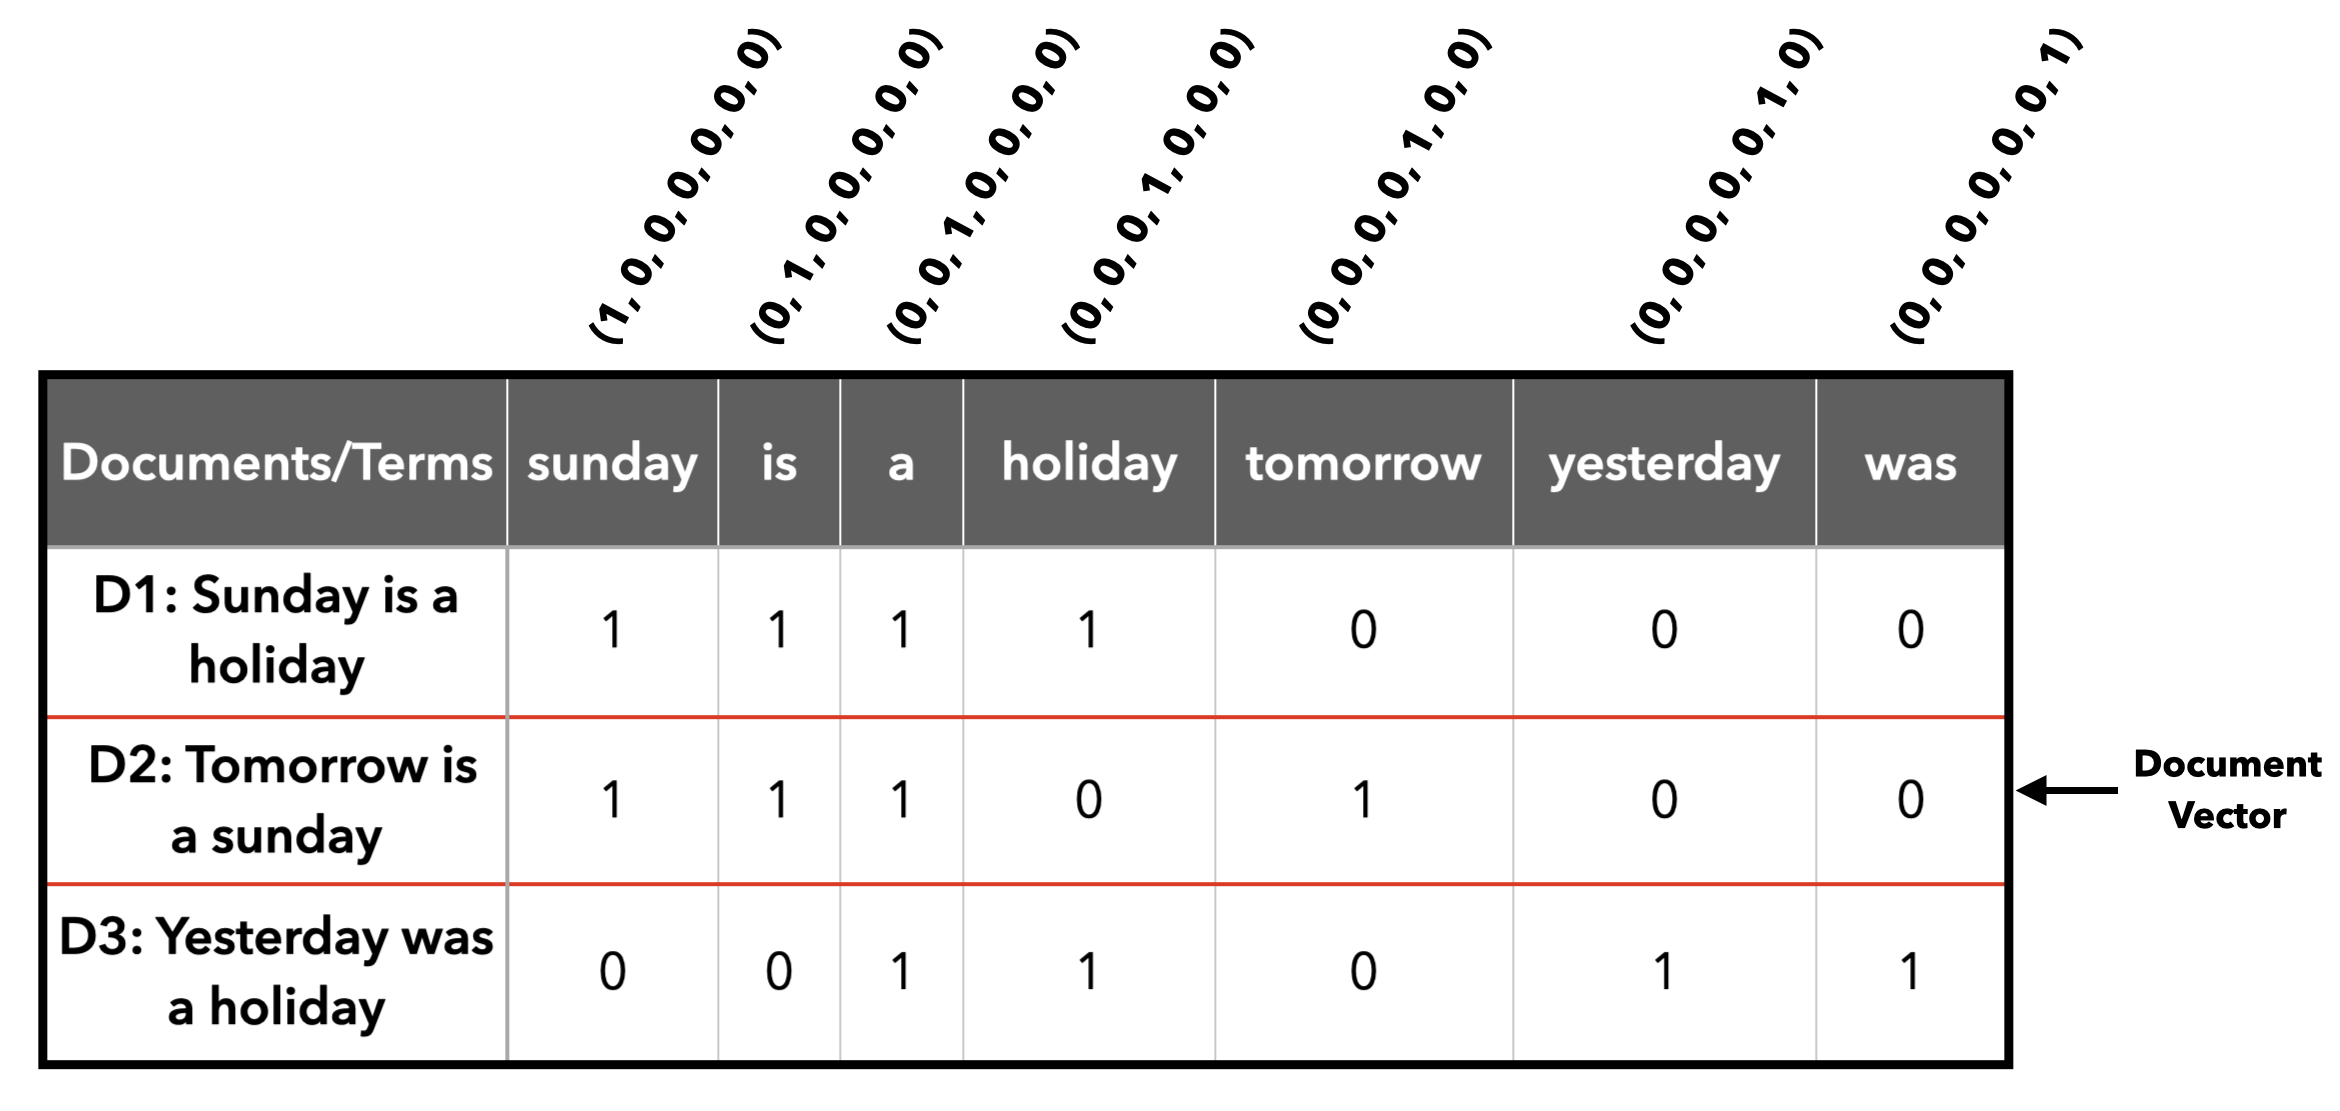
\includegraphics[width=.9\textwidth]{images/thesis_images/term_document_matrix.png}
	\caption[Term-Document matrix example.]{Term-Document matrix representing word and document vectors. \label{fig:td_matrix}}
\end{figure}


To address the limitations of solely relying on word frequency and to take into account the relationship between documents in the corpus, an improved version of the \ac{BoW} approach called \ac{TF-IDF} has been introduced. In this modeling technique, the frequency of a word in all documents across the corpus is taken into consideration, in addition to the term frequencies (or their normalized versions) within individual documents~\cite{lavin2019analyzing}. Terms that appear frequently in many documents are penalized with \ac{TF-IDF}, leading to a more effective weighting score that better reflects their importance in distinguishing documents.

The previous two approaches have limitations as they disregard word order, meaning, and are dependent on the corpus vocabulary. Furthermore, computational challenges can arise when the vocabulary size reaches millions. However, the emergence of \ac{DL} techniques has revolutionized document representations by addressing these limitations. This improvement is achieved through the utilization of semantic word representations that consider word meanings and embed vectors in a continuous vector space, rather than a discrete vector denoting a single dimension~\cite{mikolov2013efficient, pennington2014glove}. These advancements have significantly enhanced the quality of document representations.

Tomas Mikolov et al.~\cite{mikolov2013efficient} proposed an unsupervised training approach involving two model architectures for generating high-quality semantic word vectors. These architectures, known as the \ac{CBOW} and continuous skip-gram models, treat a text document as a continuous sequence of words and uses a window of words. These models operate by considering either the context words or the current word at a given time. A window is defined, spanning the length of the context words. The \ac{CBOW} architecture predicts the probability of the current word given the surrounding context words, while the skip-gram architecture predicts the probability of context words given the current word~\cite{mikolov2013efficient}. Words sharing the same context in the corpus are represented in close proximity to each other within the continuous vector space. Both architectures use a 2-layer feed-forward neural network to generate distributed representations for all words in the corpus. A projection layer is used during tuning instead of a non-linear hidden layer, which is shared across all words.


The above architectures have shown great results representing the semantics of the words. For instance, the vector equation ``king - man + woman = queen'' shows the advancement of word representations in the vector space. However, these architectures primarily focus on local context, which refers to the relationships between words that occur together within a given context or co-occurrences. The consideration of global context is lacking in both the \ac{CBOW} and skip-gram architectures. To address this limitation, Pennington et al.~\cite{pennington2014glove} proposed an approach called \ac{GloVe}. \ac{GloVe} is an unsupervised algorithm that generates distributed word representations by leveraging both local and global word-word co-occurrences. It employs a global log-bilinear regression model that combines techniques of global matrix factorization and local context window. \ac{GloVe} embeddings have exhibited superior performance compared to \ac{CBOW} and other models in tasks such as named entity recognition and word similarity~\cite{pennington2014glove}.

Polysemy refers to the phenomenon where a word or sign has multiple meanings. For example, the word "bank" can represent various concepts such as a river bank or a financial institution. Polysemy creates a significant challenge in both the Word2Vec and \ac{GloVe} approaches as they ignore the possibility of words having different semantics. To tackle this issue, the concept of contextual word embeddings was introduced by \ac{ELMo}~\cite{peters2018deep}. \ac{ELMo} word representations are generated based on the complete sentence rather than a fixed window context. Additionally, word embeddings are derived from the internal states of a bidirectional Language Model (biLM)~\cite{peters2018deep}. \ac{ELMo} also incorporates character convolutions, allowing the model to handle word representations for out-of-vocabulary words. However, Jacob Devlin et al.~\cite{devlin2018bert} argued that the \ac{ELMo} token representations generated by combing left-to-right and right-to-left biLM representations lack deep bidirectionality.


To generate deeply bidirectional word representations, an approach named \ac{BERT} ~\cite{devlin2018bert} is proposed. \ac{BERT} utilizes the transformer architecture which incorporates multi-head attention to efficiently compute embeddings in a vector space. The transformer architecture uses a self-attention mechanism with an encoder-decoder structure to generate input and output representations~\cite{vaswani2017attention}. In its pre-training phase, \ac{BERT} utilizes two techniques: \ac{MLM} and \ac{NSP}. \ac{MLM} randomly masks tokens from the input sequence and predicts the probability of the missing tokens based on their context. This random masking allows \ac{BERT} to produce truly deep bidirectional representations~\cite{devlin2018bert}. Additionally, the \ac{NSP} technique creates sentence pairs and jointly pre-trains the representations of these text pairs by predicting the next sentence given a particular sentence.


\subsection{Sentence Embeddings}

Sentence embeddings serve as numerical representations of text documents, such as sentences or paragraphs. These representations have a significant importance in \ac{IR} particularly in semantic search. A simple approach to generate sentence embeddings involves computing the mean vector representation of the words within a sentence or paragraph (with stopwords removed). However, this approach lacks the semantic coherence among words and inadequately represents the contextual information in the continuous space. In recent years, several approaches for encoding sentences have been proposed, but this section focuses on discussing two widely recognized techniques.

\begin{description}
	\item [\ac{SBERT}]  \hfill \\ The \ac{BERT} encoder is responsible for generating input representations for a sequence of tokens, which can consist of either a single sentence or two combined sentences~\cite{devlin2018bert}. \ac{BERT} incorporates special tokens to identify specific features within the input sequence. For example, the ``[SEP]'' token is utilized to separate two adjacent sentences. Rather than working on a single sentence level, \ac{BERT} operates on token-level embeddings as input. Consequently in the task of semantic similarity, all possible combinations of sentences must be supplied to the \ac{BERT} network which results in a significant computational burden~\cite{reimers-2019-sentence-bert}. Reimers and Gurevych~\cite{reimers-2019-sentence-bert} have highlighted the drawback of \ac{BERT} in generating independent sentence embeddings.
	
	A modification to the pre-training stage of \ac{BERT} called \ac{SBERT} has been proposed to directly generate sentence representations for a given input sentence. \ac{SBERT} incorporates siamese and triplet networks to update the network weights, resulting in the generation of semantically similar sentence embeddings~\cite{reimers-2019-sentence-bert}. Notably, the pre-training of the \ac{SBERT} model alone is sufficient and does not require any additional inference networks to generate the desired sentence representations. These \ac{SBERT} sentence embeddings can be readily applied in various \ac{NLP} tasks, including semantic text similarity, text classification, and text clustering. The models based on the architecture of \ac{SBERT} can be accessed using the sentence-transformers Python library\footnote{\url{https://pypi.org/project/sentence-transformers/}}.
	
	\item [Universal Sentence Encoder (USE)]  \hfill \\ The \ac{USE} is a pre-trained deep learning model developed by tensorFlow, designed to encode text data such as sentences, phrases, or paragraphs into distributed semantic vectors~\cite{cer2018universal}. Two variants of \ac{USE} models have been proposed based on their performance. One model utilizes the transformer architecture, while the other uses the \ac{DAN}. Similar to \ac{SBERT}, \ac{USE} also enables transfer learning using sentence embeddings and eliminates the need for additional inference. Transfer learning experiments conducted with both architectures have demonstrated that the transformer model outperforms \ac{DAN} across various transfer learning tasks, but it requires higher computational resources.
	
	TensorFlow introduced two new multi-lingual \ac{USE} models that are capable of embedding text from sixteen different languages into a single semantic space~\cite{yang2019multilingual}. One of these models utilizes the transformer architecture, while the other uses a convolutional neural network architecture. The \ac{USE} framework utilizes a multi-task dual encoder training approach and enables the deep learning model to train on multiple languages simultaneously~\cite{yang2019multilingual}. In this master thesis, the \ac{USE} model with the transformer architecture from \emph{Tensorflow Hub}\footnote{\url{https://tfhub.dev/google/universal-sentence-encoder-multilingual-large/3}} is utilized. According to tensorflow hub, this particular \ac{USE} model is optimized for processing multi-word text elements, such as sentences, phrases, or short paragraphs, and it does not require explicit language specification. The proposed approach uses the \ac{USE} model in various ways, including document representation, keyword extraction, and semantic document retrieval. The detailed usage of the \ac{USE} model are further elaborated in the subsequent chapters.

	
\end{description}

\section{Neural Ranking Encoders}

Neural ranking encoders refer to deep learning models that rank documents based on their relevance to a given search query. Among these models, BERT-based neural ranking models have gained significant popularity and are typically categorized into two distinct types: \emph{Bi-encoder} and \emph{Cross-encoder} models~\cite{choi2021improving, jung2022semi, ishihara2022nikkei}. The differentiation between these models lies in the encoding process of both the search query and the documents. \prettyref{fig:neural_reranker} illustrates the architectural differences between these two models.

\begin{figure}[h]
	\centering
	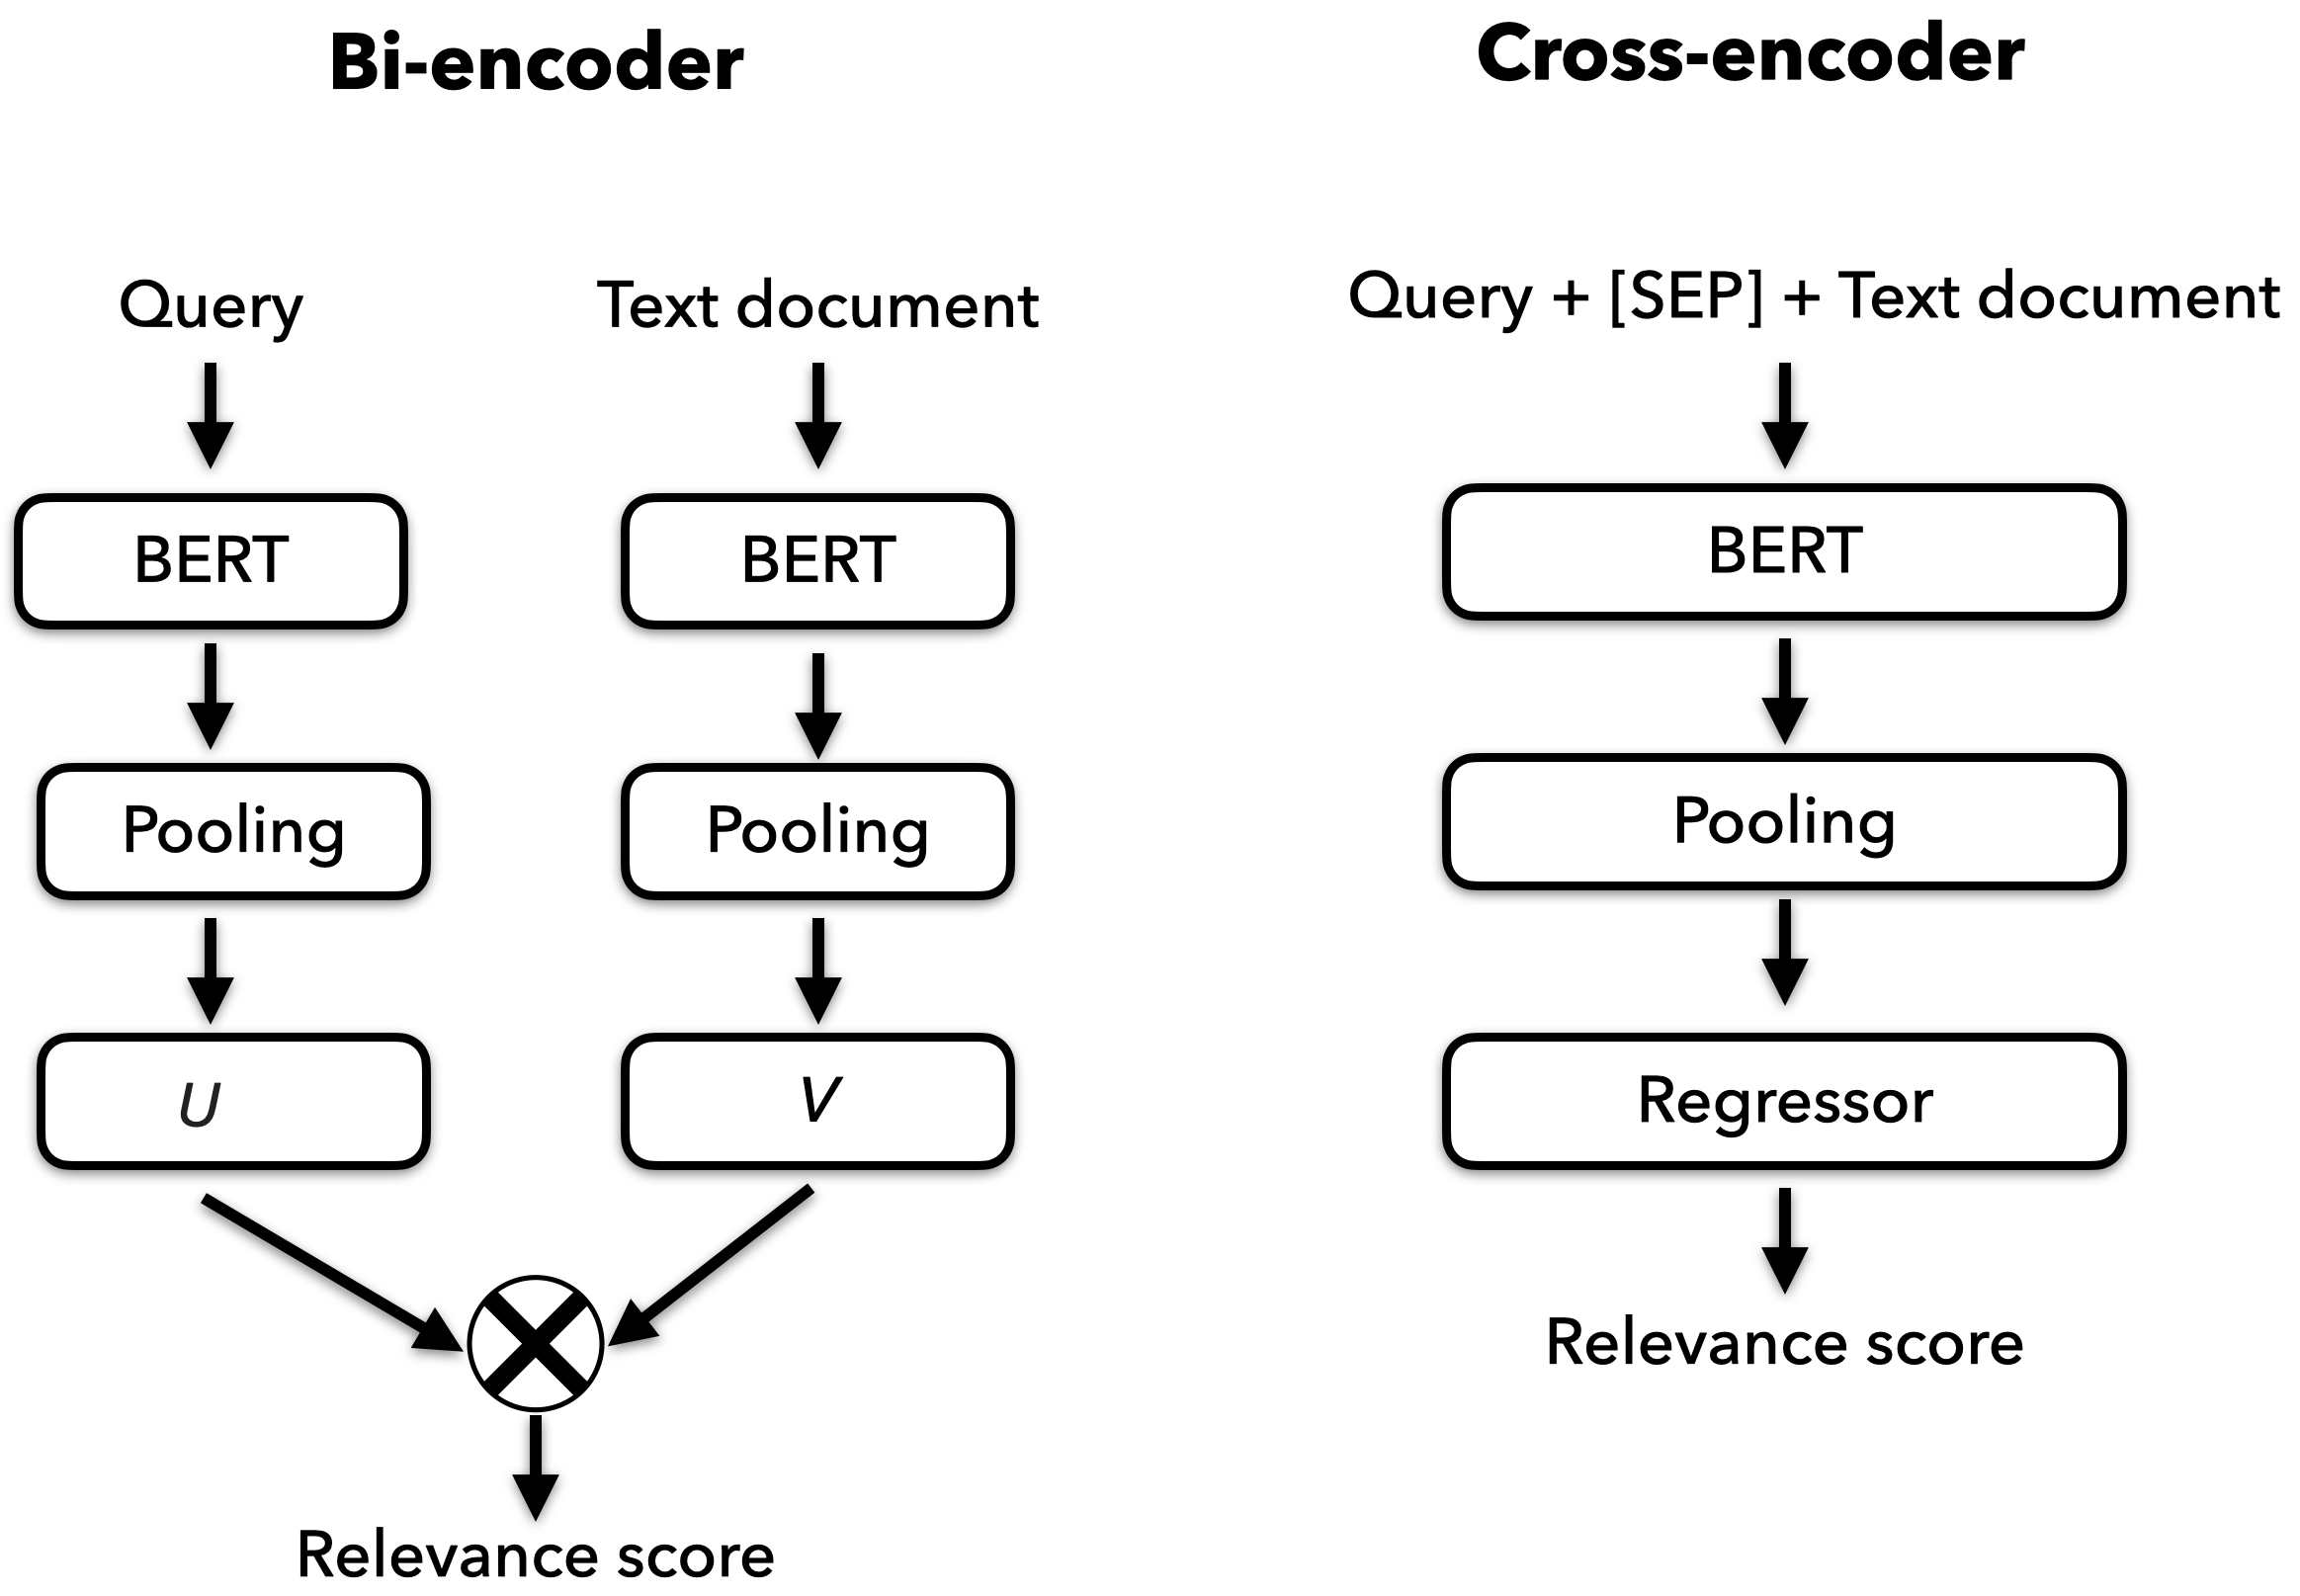
\includegraphics[width=.8\textwidth]{images/thesis_images/neural_ranking_models.png}
	\caption[Bi-encoder and cross-encoder model architectures.]{Bi-encoder and cross-encoder model architectures~\cite{ ishihara2022nikkei}. \label{fig:neural_reranker}}
\end{figure}

\begin{description}
	\item[Bi-encoder]  \hfill \\ Bi-encoder models are neural network architectures that encode the query and documents independently without considering their contextual relationship. In BERT-based bi-encoder networks, separate self-attentions are performed for the query and documents which results in separate dense representation vectors for the query and documents~\cite{choi2021improving}. To measure similarity, an external metric like Euclidean distance or cosine similarity must be used.
	 
	\item[Cross-encoder]  \hfill \\ On the other hand, cross-encoder models are neural network architectures that considers the contextual relationship between the query and documents during the encoding process. In BERT-based cross-encoder networks, a full self-attention mechanism is applied to the query and document pair with a separation token (``[SEP]'') between them~\cite{choi2021improving}. Pre-trained cross-encoder models directly assign a relevance score to the query within the range of [-1, 1].
	
\end{description}

Both the above-mentioned ranking models can be used for \ac{IR}, question-answering, and other related tasks. Cross-encoders generally show superior performance compared to bi-encoders, but requires more computational resources for training or fine-tuning~\cite{choi2021improving, jung2022semi}. This master thesis exclusively uses pre-trained BERT-based ranking encoders. Neural ranking models are employed specifically for comparing the proposed approach with existing literature. Further details on the usage of these encoders are provided in subsequent chapters.

\section{Automatic Keyword Extraction}

Beliga~\cite{beliga2014keyword} has described keyword extraction as the automatic identification of terms that best represent the most relevant information in the document. Keyword extraction techniques are mainly classified into unsupervised or supervised approaches~\cite{bennani2018simple}. Supervised keyword extraction approaches require many labeled datasets containing both documents and keywords from each document. Manual annotation of keywords from each document is a very expensive and tedious task~\cite{beliga2014keyword}, depending on the length of the documents. On the other hand, unsupervised approaches do not require any labeled information but often have poor accuracy~\cite{bennani2018simple}.


\begin{figure}[h]
	\centering
	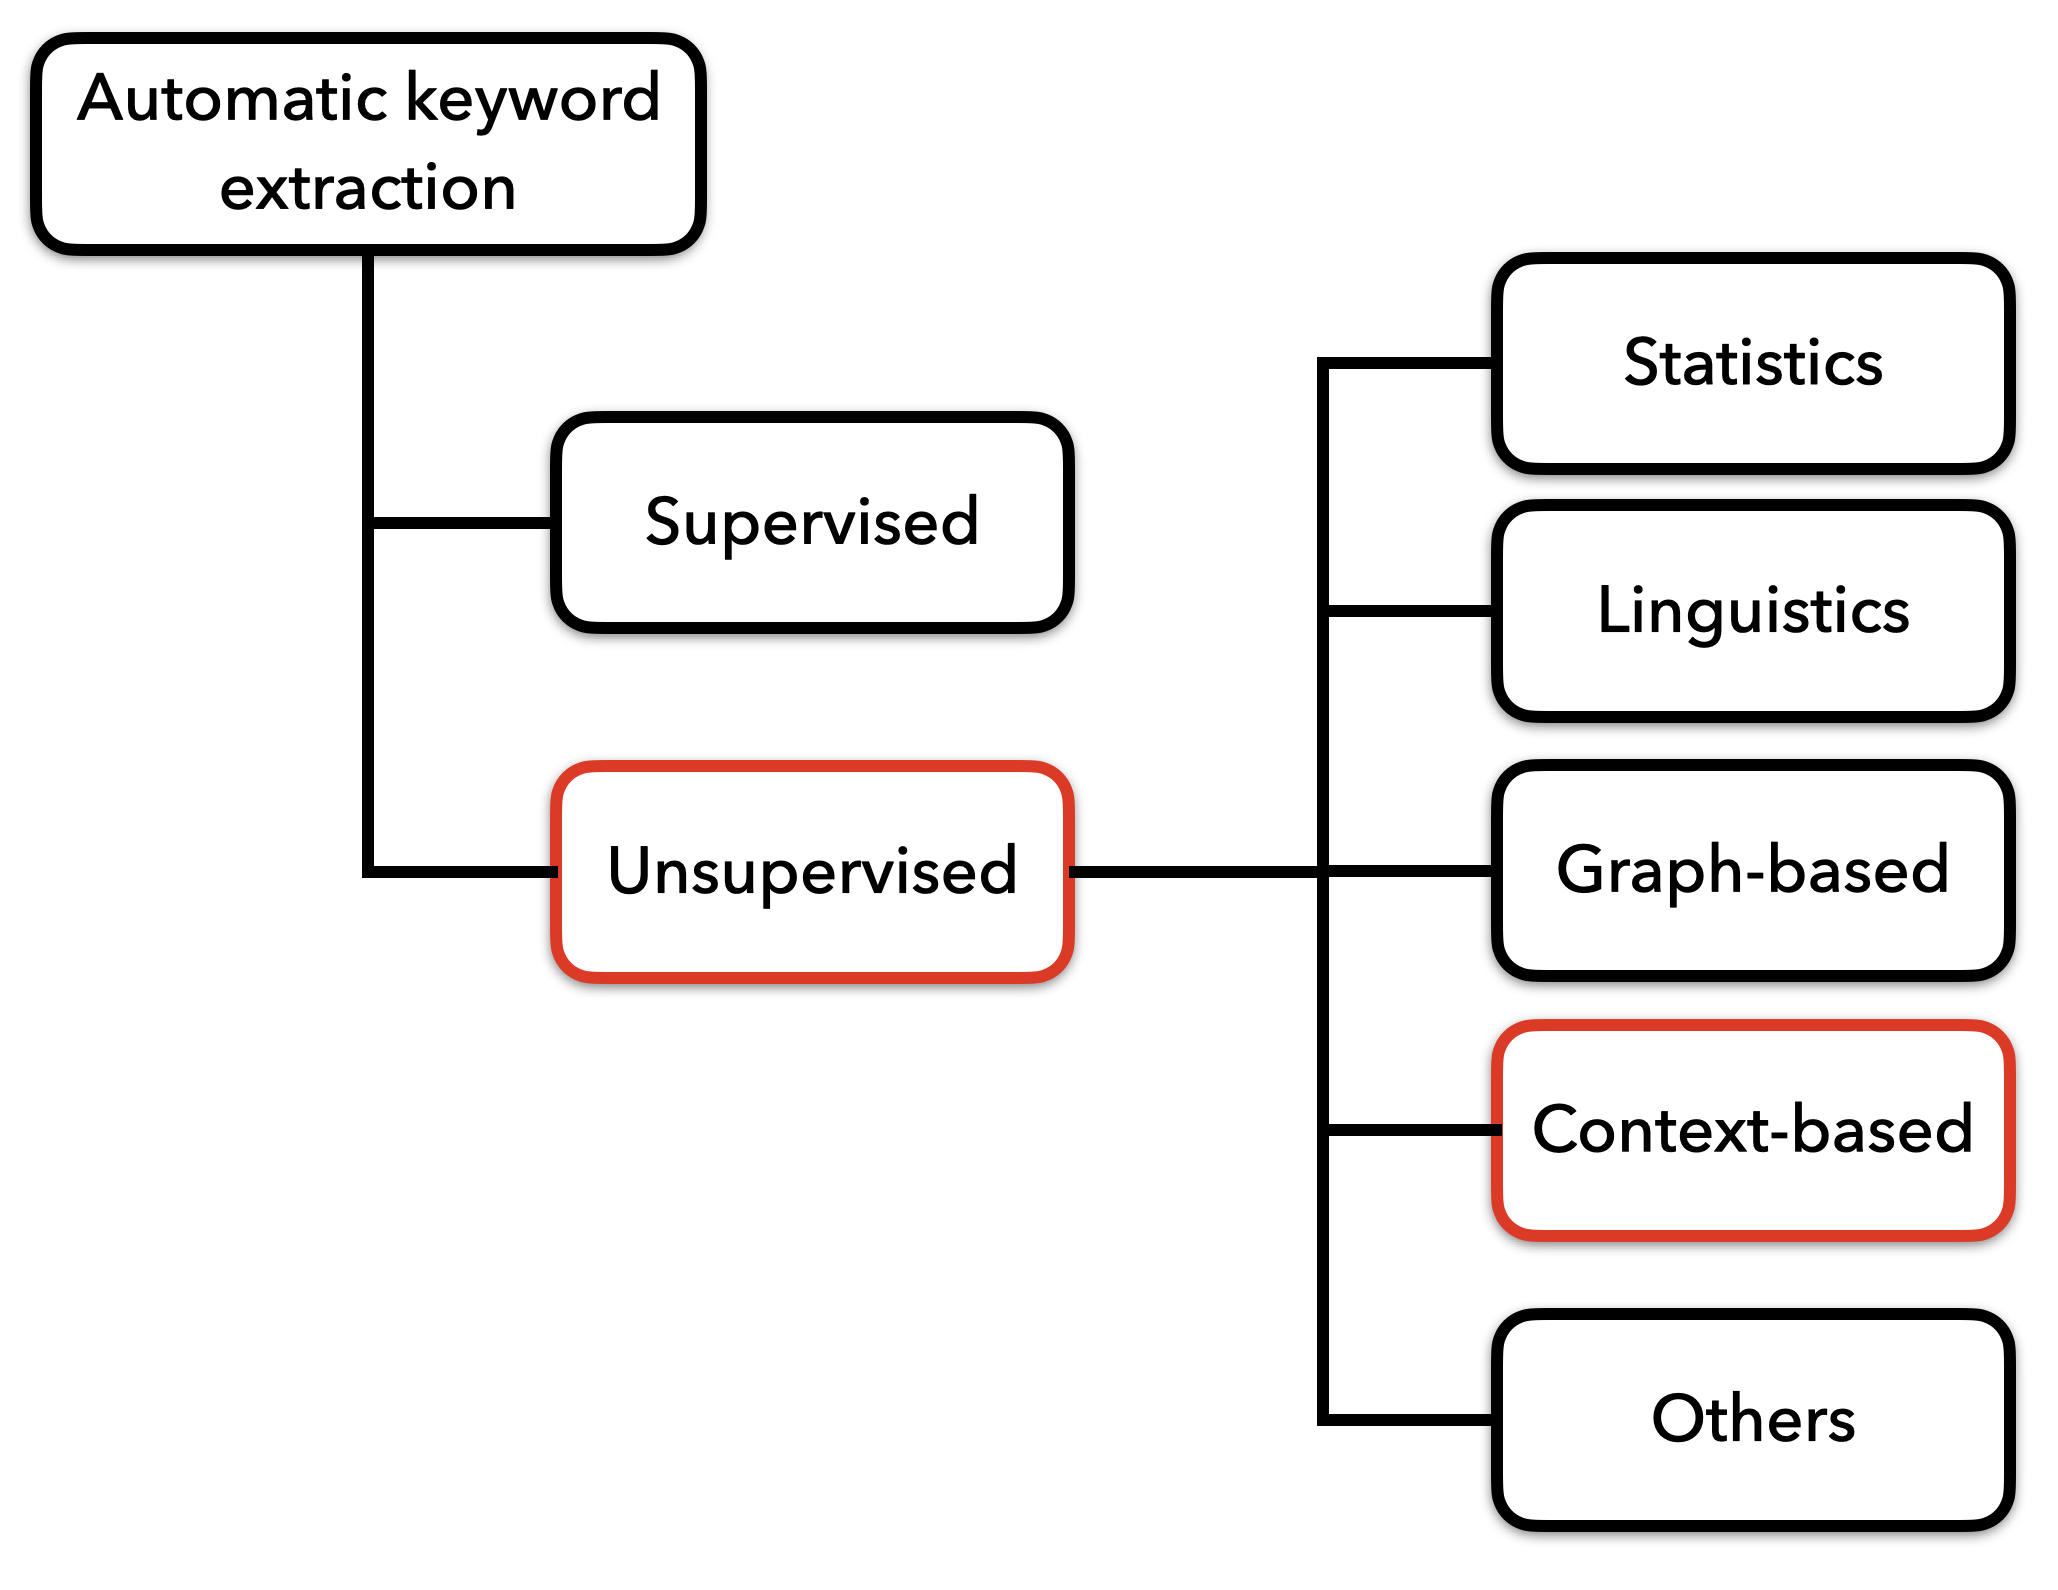
\includegraphics[width=.6\textwidth]{images/thesis_images/keyword_extraction_techniques.png}
	\caption[Keyword extraction techniques.]{Categorization of automatic keyword extraction techniques. \label{fig:keyword_extraction_techniques}}
\end{figure}

Despite the poor accuracy, an unsupervised approach is chosen for extracting keywords in this master thesis as it is difficult and expensive to build a keyword dataset from very long text documents. Some of the popular unsupervised approaches are highlighted in \prettyref{fig:keyword_extraction_techniques}. Statistics-based approaches make use of information such as word frequencies, \ac{TF-IDF}, word co-occurrences, etc.~\cite{beliga2014keyword}. This statistical information is extracted either from an individual document or at the corpus level. Linguistic-based techniques use features that represent the language, such as information related to lexicon, syntax, semantics, etc., to extract keywords~\cite{beliga2014keyword}. On the other hand, graph-based keyword extraction approaches model a document as a graph, where terms are vertices of the graph and the relations between the terms are edges. 

Statistical and linguistic-based features between the terms can be used to represent the edges of the graph. Graph-based approaches perform better than earlier approaches by effectively exploring term relationships~\cite{beliga2014keyword}. In this master thesis, an approach to select keywords based on contextual embeddings is chosen. This approach is inspired by recent research related to using contextualized sentence embeddings for keyphrase extraction, namely \emph{EmbedRank}~\cite{bennani2018simple}. Bennani-Smires et al.~\cite{bennani2018simple} have shown that the EmbedRank approach has performed better than state-of-the-art graph-based keyword extraction approaches. To generate phrase embeddings of the noun chunks and the original news article, a multi-lingual pre-trained \ac{USE} from tensorFlow is employed. 


\section{Dimensionality Reduction}

Sentence or word embeddings are very high-dimensional distributed vectors, especially \ac{USE} embeddings have a dimension size of 512. Data processing tasks such as visualization, data analysis, feature extraction, clustering, etc., on data with high dimensions can be computationally expensive. Therefore, the dimensions of the data are reduced for all the data points in the dataset without losing crucial patterns or information. This technique is generally referred to as dimensionality reduction. Many dimensionality reduction techniques have been proposed in recent years, and they can be categorized into two types. Algorithms that preserve the pairwise distance structure among all the data points in the dataset~\cite{mcinnes2018umap}. One example in this category is \ac{PCA}. \ac{PCA} assumes that the data is linear and does not perform well in the case of data with non-linear relationships. The other type of algorithms considers the non-linear relationships in the data and preserves local or global structures in the data. One example of these non-linear algorithms is \ac{UMAP}.


\begin{figure}[h]
	\centering
	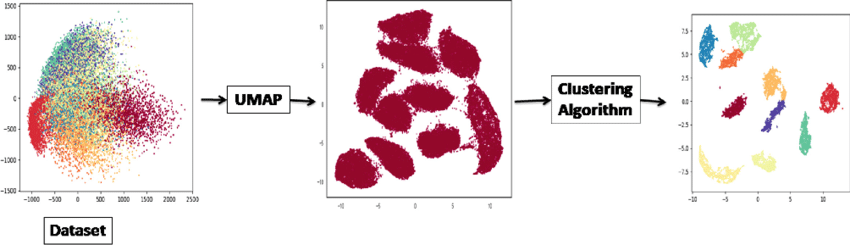
\includegraphics[width=.9\textwidth]{images/papers/umap.png}
	\caption[UMAP pipeline for clustering.]{Improved clustering pipeline after reducing the data dimensions~\cite{allaoui2020considerably}.  \label{fig:umap}}
\end{figure}

Allaoui et al.~\cite{allaoui2020considerably} have observed an increase in the performance of clustering methods after dimensionality reduction on the data using \ac{UMAP}, as shown in \prettyref{fig:umap}. They tested a few popular clustering techniques such as k-means, gaussian mixture models, agglomerative hierarchical clustering, and \ac{HDBSCAN}, and observed an increase in accuracy after \ac{UMAP} dimensionality reduction. Moreover, the time taken for clustering was drastically reduced. \ac{UMAP} works based on \emph{Riemannian geometry and algebraic topology}, preserving the global structure in the data~\cite{mcinnes2018umap}. One of the main reasons for the acceptance of \ac{UMAP} in \ac{ML} is its computational efficiency, though it is slower than \ac{PCA}~\cite{umaplearnPerformanceComparison}. However, given the quality of reduced representations and its ability to handle the non-linear relationships in the data, \ac{UMAP} is clearly a viable dimensionality reduction technique in \ac{ML}. In this master thesis, \ac{UMAP} is used to reduce the dimensionality of the data.



\section{Document Clustering}

\ac{DC} is the task of separating documents into meaningful groups where the documents with similar characteristics belong to a similar group. In addition to \ac{DC}, the task of topic modeling is also referred to in order to achieve the same outcome. \ac{DC} plays a crucial role in the field of big data and data mining. Generally, clustering is performed on numerical data points in the continuous space. However, text documents are in alphanumeric format (including some special characters). One of the earliest approaches to represent text documents is the \ac{BoW} method and \ac{TF-IDF} weighting, which is described in Section 3.1.1. Two main disadvantages of these methods are the lack of semantic representation and high-dimensional representation. Since the dimensions depend on the number of words in the corpus, this can lead to computational overhead. Semantic (contextual) text representations, with the help of word or sentence embeddings, encode the text in fixed-length vectors. There are several clustering techniques tested on text document clustering, such as partitioning, hierarchical, and density-based~\cite{afzali2019text}. Below are a few clustering algorithms discussed at an abstract level, and their advantages and disadvantages are highlighted.


\begin{description}
	
	\item [Partitioning clustering]  \hfill \\ 
	This type of clustering deals with creating a fixed number of clusters of similar data based on a particular criterion. K-means clustering is one of the popular and simple clustering techniques based on distance measurement in \ac{ML}. The K-means algorithm partitions the data of $n$ samples into $k$ clusters using a centroid-based iterative approach~\cite{afzali2019text}. Being a parametric clustering approach, the number of clusters $k$ needs to be well designed according to the data. One major drawback is the cluster shape, as the algorithm expects a spherical or circular shape output due to the centroid approach. K-means also does not assume any inherent noise in the data and assigns all data points to a cluster.
	
	
	\item [Hierarchical clustering]  \hfill \\ These clustering algorithms create a hierarchical structure from the data samples. There are two types of hierarchical clustering methods, namely the top-bottom/divisive approach and the bottom-top/agglomerative approach~\cite{afzali2019text}. In the top-bottom approach, all data samples are considered to be a single cluster, and this cluster is further decomposed into smaller clusters until a certain criterion is achieved. Conversely, in the bottom-top approach, each data sample is considered as a single cluster, and the clusters are merged to form larger clusters until a certain criterion is met~\cite{zhao2002comparison}.
	
	
	Agglomerative hierarchical clustering is one of the popular hierarchical algorithms in \ac{ML}, and unlike k-means, there is no need to specify the number of clusters before clustering. However, extensive experiments comparing both clustering algorithms show that partitioning clustering always performs better than agglomerative clustering~\cite{zhao2002comparison}. The authors also suggest to use partitional clustering for large document collections.

	
	\item [Density based clustering]  \hfill \\ Similar to hierarchical clustering, density-based clustering methods are non-parametric and separate data samples into clusters based on high-density areas until a certain criterion is met. Density can be interpreted as the number of points located within a certain region. \ac{DBSCAN} is one of the popular density-based clustering algorithms. \ac{DBSCAN} characterizes every data point as either a core point, a border point, or a noise point~\cite{campello2020density}. Two crucial parameters in the \ac{DBSCAN} algorithm are $\epsilon$ (epsilon) and $minPts$ (minimum number of points). A data point is defined as a core point when it contains neighboring datapoints higher than $minPts$ within a circle of radius $eps$.
	
	
	\begin{figure}[h]
		\centering
		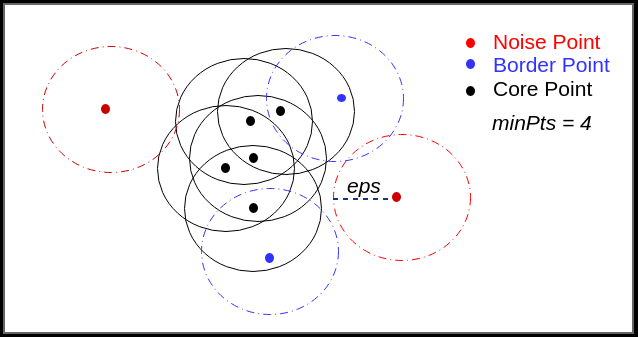
\includegraphics[width=.6\textwidth]{images/papers/dbscan.png}
		\caption[DBSCAN classification of data points.]{DBSCAN classification of data points~\cite{knoldusDBSCANClustering}. \label{fig:dbscan}}
	\end{figure}
	
	A density-based cluster is expressed as a maximally connected component of the data points that lie within a distance less than $eps$ from a core point (as described above)~\cite{campello2020density}. Border points are data points inside a cluster that do not follow the core point property. Data points that are not part of a cluster and do not follow the core point criteria are noise points. Different data points are presented visually in \prettyref{fig:dbscan}. There are more parameters in this algorithm that define the final clustering output, but the number of clusters is not a parameter. This helps the algorithm assign the number of clusters according to the given data.

	
	Density-based clustering clearly has many advantages compared to other clustering algorithms, such as efficient noise handling, non-parametric nature, and flexible clusters (with no specific shape and size). However, \ac{DBSCAN} has limitations, such as difficulty in parameter selection and handling varying density clusters~\cite{mcinnes2017accelerated}. To overcome these limitations, an algorithm called \ac{HDBSCAN} was proposed. This clustering algorithm extends \ac{DBSCAN} by removing the concept of border points and exploring different values of $eps$. 
	
		\begin{figure}[h]
		\centering
		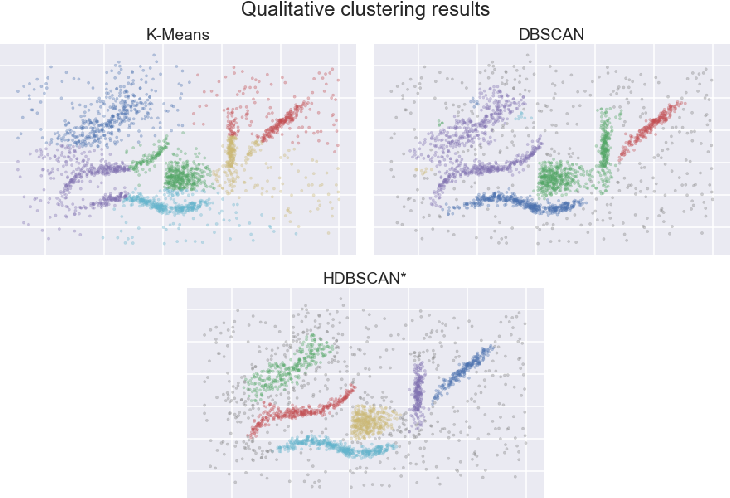
\includegraphics[width=.8\textwidth]{images/papers/hdbscan.png}
		\caption[K-means vs DBSCAN vs HDBSCAN.]{Comparison of clustering results from three algorithms namely k-means, DBSCAN, HDBSCAN~\cite{mcinnes2017accelerated}.  \label{fig:hdbscan}}
	\end{figure}
	
	
	
	A hierarchy of different \ac{DBSCAN} clusterings is generated using different values of $eps$~\cite{mcinnes2017accelerated}. The hierarchy is condensed and used to determine the clustering output, which provides stability for $eps$. To achieve this, a new parameter named \emph{minimum cluster size} is introduced. In this way, \ac{HDBSCAN} overcomes the limitation of handling varying densities, and there is no need to explicitly select the parameter $eps$. In \prettyref{fig:hdbscan}, the results from three clustering algorithms are presented, and it can be observed that \ac{HDBSCAN} handles both low-density noise points and high-density clusters very well. However, \ac{HDBSCAN} is computationally slower compared to \ac{DBSCAN}.

	
	

	
\end{description} 


Clustering algorithms can be further characterized into two types, namely hard clustering and soft clustering, depending on the clustering output~\cite{de2012document}. When the clustering algorithm strictly assigns each data point to a single cluster, it is referred to as \emph{hard clustering}. In \ac{DC}, an example of hard clustering output is when one document is assigned to one cluster. On the other hand, when the clustering output assigns a data point to several clusters, it is referred to as \emph{soft clustering}. For example, when a document is assigned to several clusters, it is an example of soft clustering.


\section{Topic Modeling}

The process of extracting inherent patterns or structures from a large collection of text documents is referred to as \ac{TM}~\cite{angelov2020top2vec}. \ac{TM} is an unsupervised \ac{ML} approach to express a text document as a mixture of topics. For example, a topic can be a general theme such as sports, politics, business, movies, health, etc. \ac{LDA} is one of the popular \ac{TM} algorithms that generates a soft-clustering output. \ac{LDA} is a generative probabilistic model that represents each document as a finite mixture of topics and each topic as a finite mixture of words~\cite{blei2003latent, angelov2020top2vec}. \ac{LDA} uses the \ac{BoW} representation, where a document is a finite set of words. One major limitation of the \ac{LDA} method is the lack of semantic representation.

\begin{figure}[h]
	\centering
	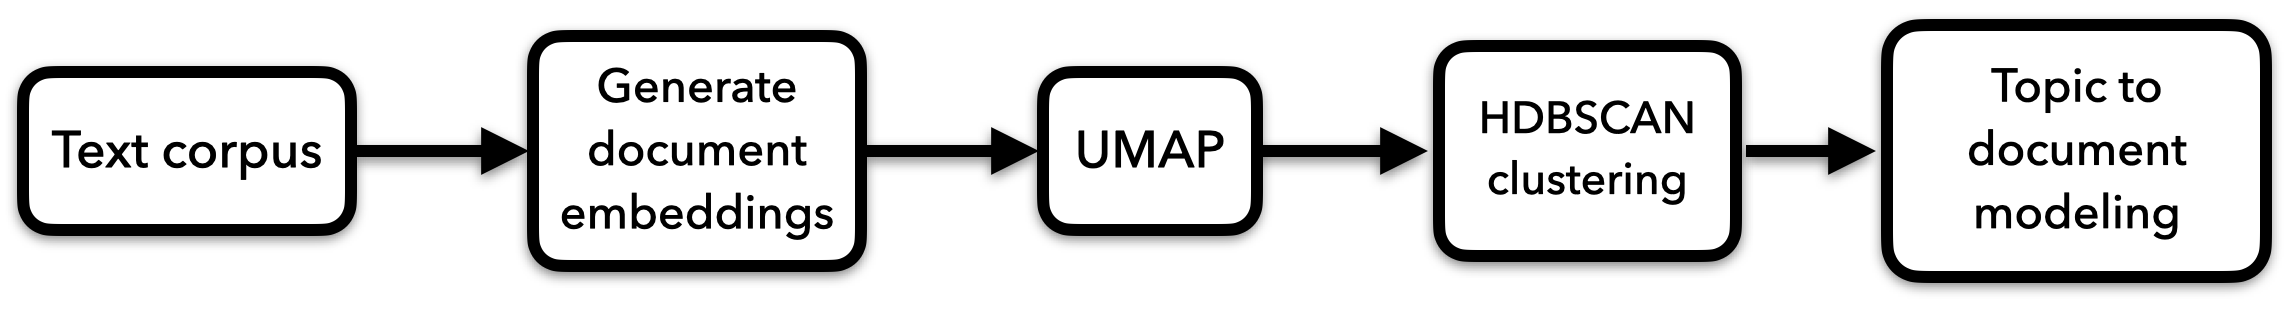
\includegraphics[width=.99\textwidth]{images/thesis_images/top2vec.png}
	\caption[Top2vec topic modeling.]{Top2vec methodology to generate semantic topic-modeling.   \label{fig:top2vec}}
\end{figure}

To overcome this limitation, a new approach called top2vec is proposed. By leveraging the distributed semantic representation of words and sentences, a text document can be represented in the continuous space. This provides an advantage in learning topics in the continuous vector space~\cite{angelov2020top2vec}. top2vec encodes the text documents into the vector space using sentence embeddings. These high-dimensional embeddings are reduced to lower dimensions using the \ac{UMAP} technique and then clustered using the \ac{HDBSCAN} algorithm. The pipeline used in top2vec is presented in \prettyref{fig:top2vec}. During clustering, the high-density areas in the semantic space are grouped together, resulting in topics being expressed as cluster centroids. The results demonstrate that top2vec identifies topics that are more informative and representative compared to the traditional topic modeling algorithm, \ac{LDA}~\cite{angelov2020top2vec}. More details about the technologies and definitions can be found in Appendix \ref{appendix:A}.










        % !TEX root = ../thesis.tex

\chapter{Related Work}

The objective of a document retrieval system is to generate a ranked list of text documents for a given user search query. To accomplish this, researchers have explored various techniques, including probabilistic frameworks, \ac{ML}, \ac{DL}, and more. These approaches aim to enhance retrieval results, often relying on the availability of labeled data. The research in this field can be broadly categorized into two types: supervised and unsupervised approaches. In the following sections, a detailed description of several approaches relevant to the subject of this master thesis is provided.

\section{Supervised Approaches}


Numerous researchers have utilized \ac{ML} algorithms with specialized loss functions that consider the relevance between search queries and documents. These algorithms, such as RankBoost~\cite{freund2003efficient} and RankNet~\cite{burges2005learning}, employ query relevance to re-rank the documents. However, acquiring labeled data with relevance information for \ac{ML} approaches can be expensive. To address this challenge, Joachims~\cite{joachims2002optimizing} proposed an approach that leverages click-through data which is generated from query-log information in search engines. More recently, state-of-the-art techniques have emerged in the form of supervised approaches using neural re-ranking methods based on sophisticated \ac{DL} architectures. These methods combine distributed word embeddings with the power of non-linear neural networks, yielding remarkable improvements in retrieval system performance by incorporating semantic considerations~\cite{mitra2017learning, guo2016deep, nogueira2019passage}.

\section{Unsupervised Approaches}

These approaches leverage unlabeled information and re-rank the retrieved results based on the user query and the top retrieved documents~\cite{rohatgi2020psu, azad2019query}. Previous approaches heavily relied on probabilistic relevance methods to rank documents. One widely used probabilistic relevance approach is BM-25, which uses a term-weighting technique to assess the relevance of documents to a given search query~\cite{robertson2009probabilistic}. One common challenge in these approaches arises from user queries, which often consist of only a few keywords~\cite{azad2019query, Kankaria2015QueryET}. To address this issue, numerous researchers have explored \ac{QE} approaches, which aim to enrich the query with additional meaning and context. \ac{QE} techniques encompass various methods such as clustering search results, query filtering, word sense disambiguation, and relevance feedback~\cite{azad2019query}. Relevance feedback involves retrieving search results using the original query provided by the user and then utilizing the top-k documents for query expansion~\cite{azad2019query}.

Researchers have explored various techniques for clustering search results, including document-level clustering, keyphrase-based clustering, and query-specific clustering~\cite{bernardini2009full, kurland2008rank, zamir1998web, osinski2005concept, liu2004cluster, liu2006representing}. Some studies have utilized distance-based clustering algorithms such as k-means, while others have experimented with hierarchical clustering~\cite{bernardini2009full, mehlitz2007new, yuan2022measurement}. Hierarchical clustering offers flexibility in adjusting the threshold level for cutting the clustering dendrogram in a bottom-up approach. However, a common limitation in many clustering approaches is the practice of assigning a document to a single cluster, which may not be logically valid since a document can contain keywords from different domains. Clustering approaches focused on the word level, such as those described in~\cite{bernardini2009full, mehlitz2007new}, typically consider only a single language or retrieval results corpus and lack a dedicated keyword selection stage. Consequently, these approaches cannot be readily applied to multilingual corpora.

Angelov~\cite{angelov2020top2vec} has made a significant advancement in document clustering by leveraging contextual embeddings from sentence encoders. This breakthrough has resulted in an efficient and interpretable topic modeling approach. In recent years, the utilization of pre-trained deep learning models has revolutionized semantic search by providing dense vector representations of text documents. A notable retrieval architecture that leverages a combination of text retrieval techniques to enhance the final document ranking is the \emph{Multi-stage ranking} architecture~\cite{yates2021pretrained, anand2021serverless, nogueira2019passage}. This architecture follows an unsupervised neural re-ranking approach, employing a \emph{Retriever} in the first stage and a \emph{Re-ranker} in the second stage. \prettyref{fig:multi-stage-ranking} shows the architecture of multi-stage ranking. 

\begin{figure}[h]
	\centering
	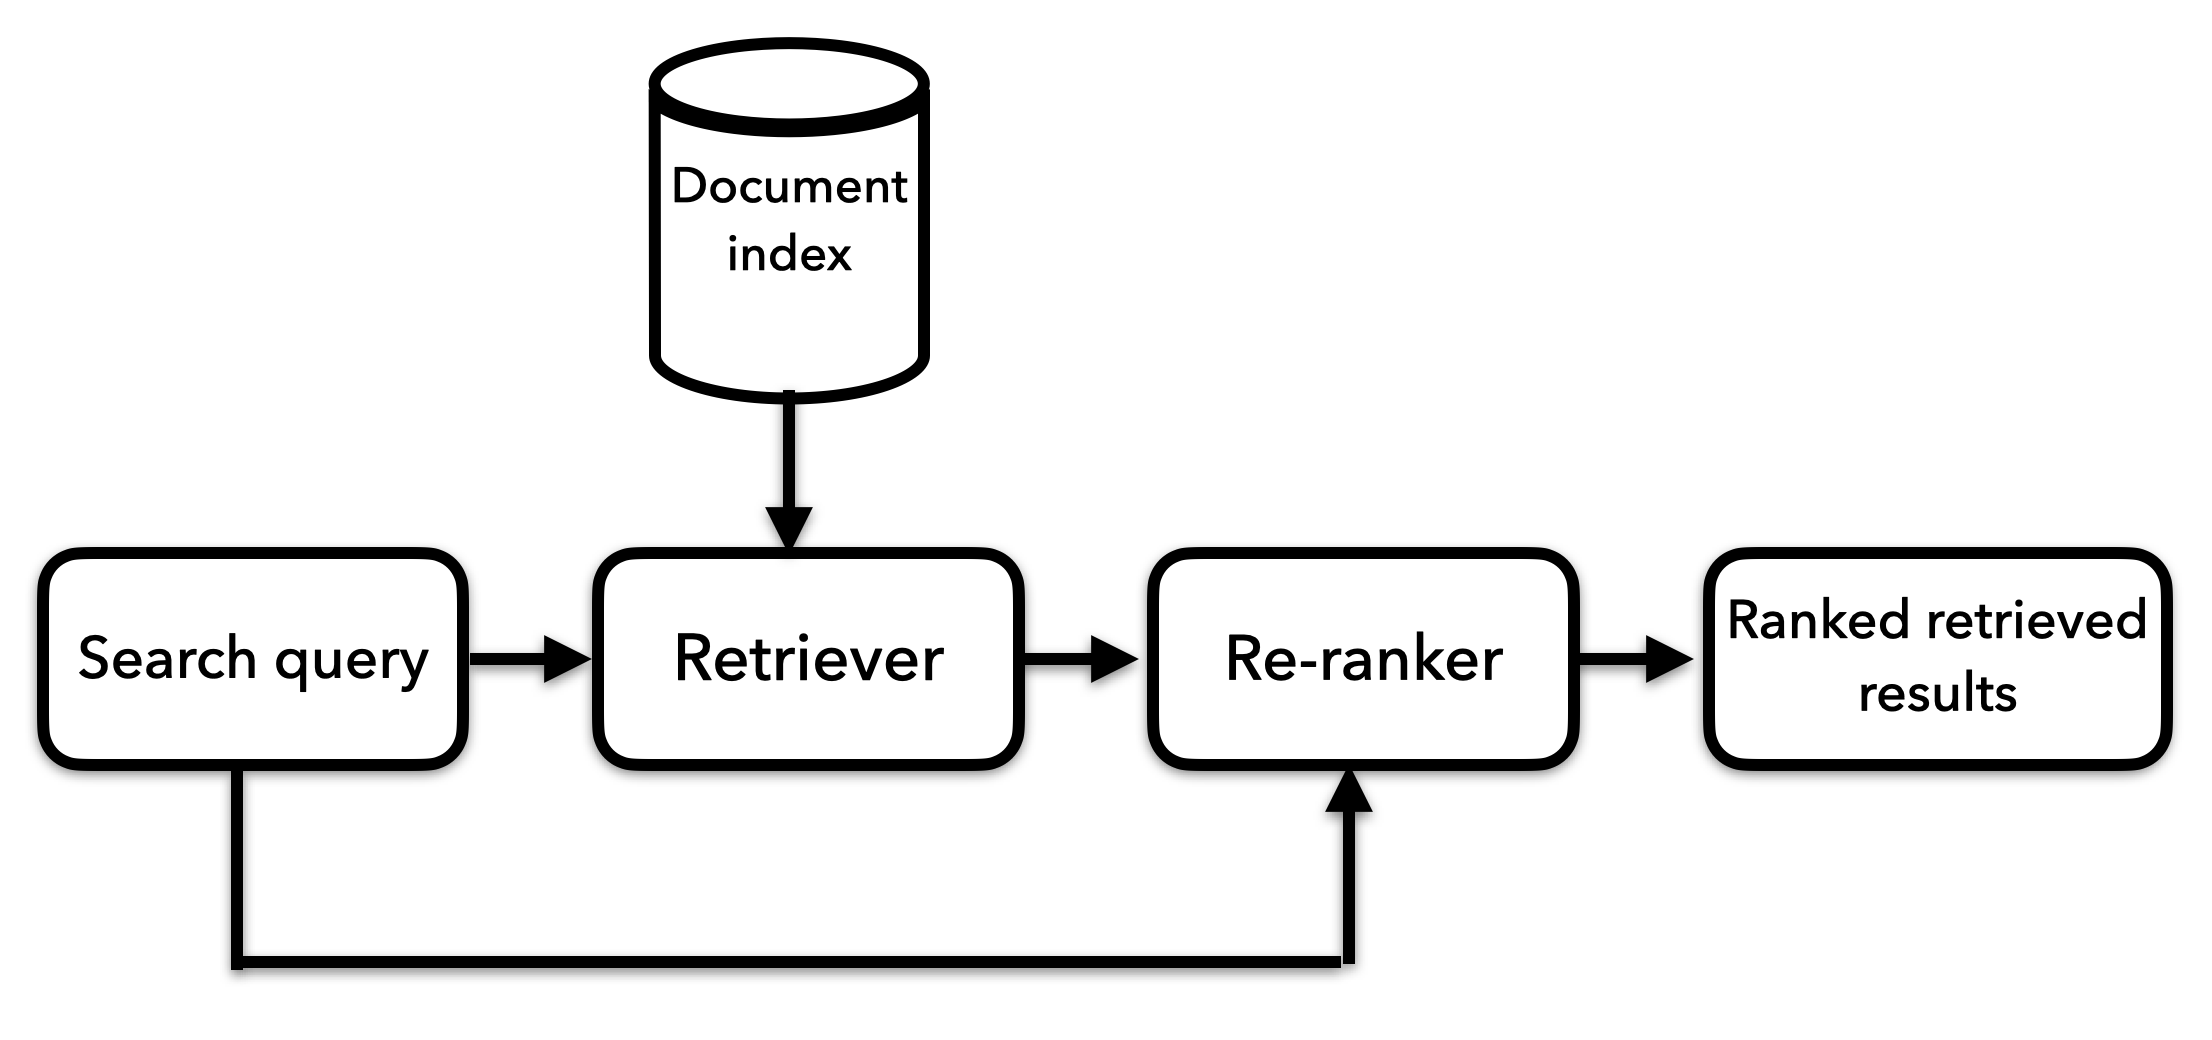
\includegraphics[width=.95\textwidth]{images/thesis_images/retriever_reranker_approach.png}
	\caption{Multi-stage ranking architecture.  \label{fig:multi-stage-ranking}}
\end{figure}

The retriever component is responsible for retrieving documents that are similar to the search query and generating a set of candidate texts for ranking~\cite{yates2021pretrained}. Various retrieval algorithms, such as BM-25 and bi-encoder semantic retrieval, can be employed at this stage. On the other hand, the re-ranker component organizes the candidate texts based on their relevance to the query~\cite{yates2021pretrained}. Re-ranker models often utilize transformer models that directly assign a relevance score to measure the alignment between the candidate text document and the query~\cite{nogueira2019passage, yates2021pretrained}. Unsupervised re-ranker models, known as cross-encoder, are pre-trained on retrieval datasets. This architecture has also been applied to enhance question-answering tasks. Malloci et al.~\cite{malloci2020text} utilized a specific candidate selection approach that filters phrases from keyword extraction by focusing on particular noun chunks. The pipeline employed in this research is illustrated in  \ref{fig:syntactic_candiate_selection}. 

\begin{figure}[h]
	\centering
	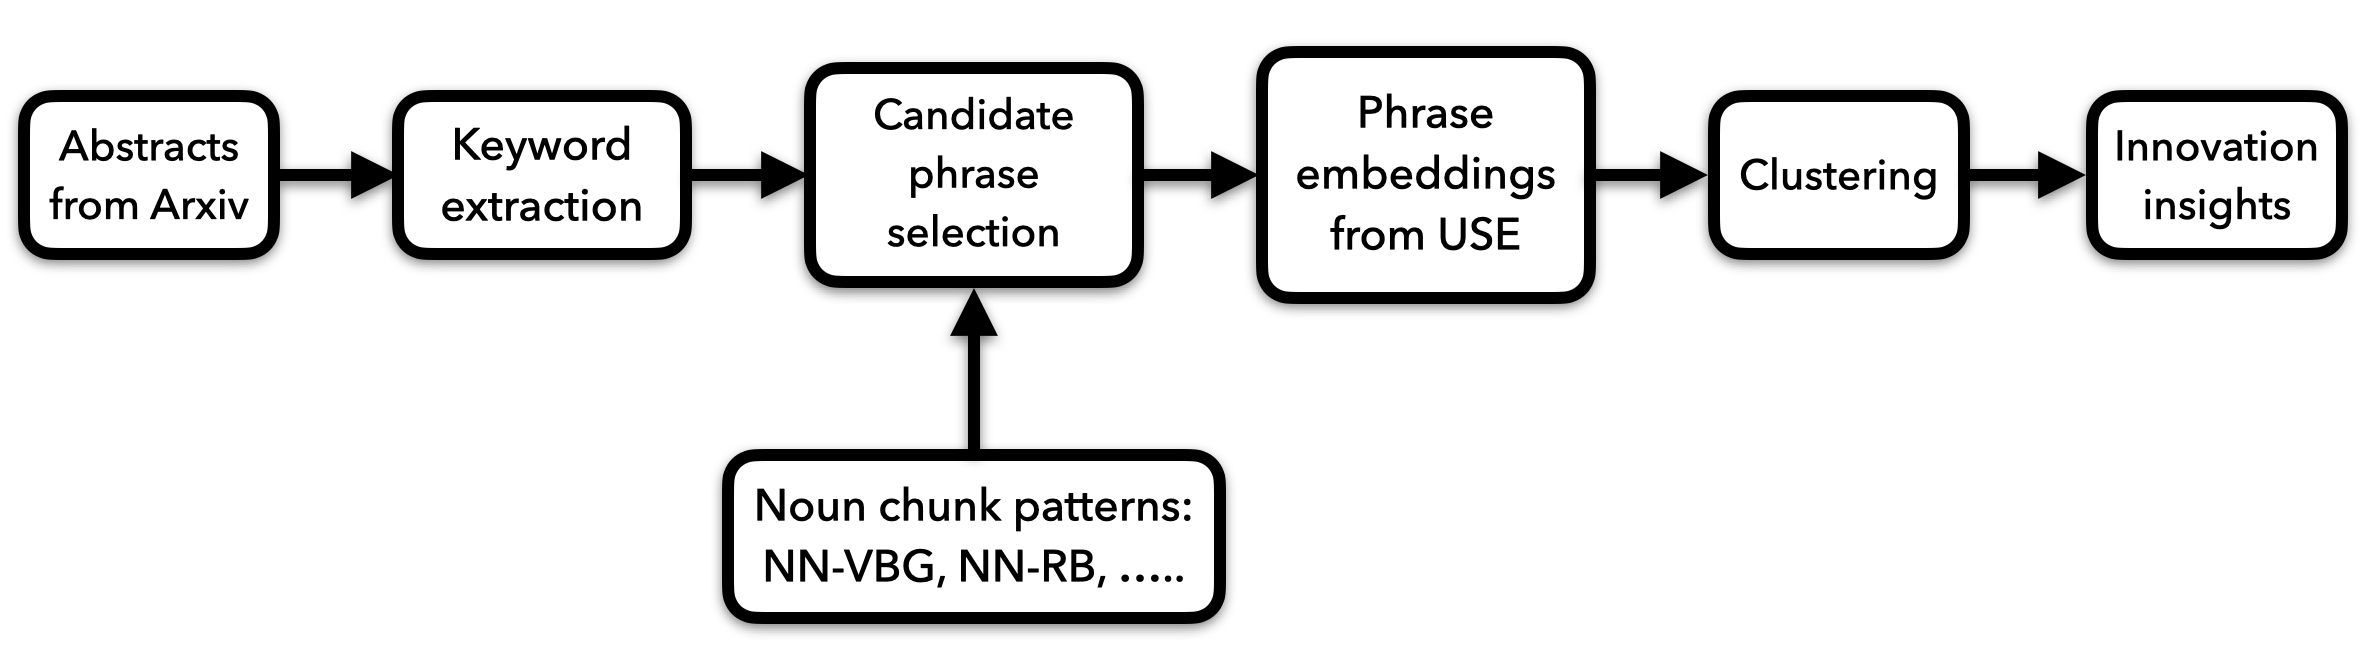
\includegraphics[width=.99\textwidth]{images/thesis_images/syntactic_candidate_selection.png}
	\caption[Innovation insights pipeline extraction.]{Pipeline to extract innovation insights using candidate selection.   \label{fig:syntactic_candiate_selection}}
\end{figure}

The primary purpose of this pipeline is to extract valuable insights related to innovation from research projects. The authors have provided detailed guidelines for selecting specific noun chunk patterns to restrict the choice of keywords used in the clustering process. However, this approach has a limitation as it lacks semantic considerations during keyword selection, which may result in the exclusion of important keywords. Given the focus on innovation at \ac{FKIE}, this master thesis introduces and evaluates a unique query-specific candidate keyword selection approach. An important observation from the literature is the effectiveness of multi-stage ranking and the utilization of vector representations for text documents.

Furthermore, the proposed approach allows for the semantic mapping of documents to specific topics and accommodates multiple languages by utilizing a single multilingual pre-trained sentence encoder. This enables the seamless integration of news articles from various languages into the document indices, without requiring any modifications to the clustering pipeline. The proposed approach can be further expanded to analyze any corpus comprising long text documents associated with a given phrase or keyword. Given the lack of labeled news articles with query and innovation relevance, an unsupervised approach is developed to establish an effective candidate document pool, facilitating efficient sub-topic creation and ranking. In subsequent sections, the proposed approach is described in detail and compared with existing literature.

    
        % !TEX root = ../thesis.tex

\chapter{Sub-topic Modeling}

One way to extract different contexts from the candidate pool is to perform clustering. This results in very abstract or generic clusters closely related to a given query and does not provide new insights to the user. To generate diverse and distinctive clusters, the latent information at the word or phrase level need to be used rather than at the document level~\cite{blei2003latent}. Since the documents contain multiple occurrences of the query and are also highly similar in semantic space, the impact of the given user query to generate a clear distinction between the documents needs to be reduced. \prettyref{fig:methodology2} illustrates the proposed approach on an abstract level to tackle the above issue and generate highly heterogeneous clusters.


\begin{figure}[h]
	\centering
	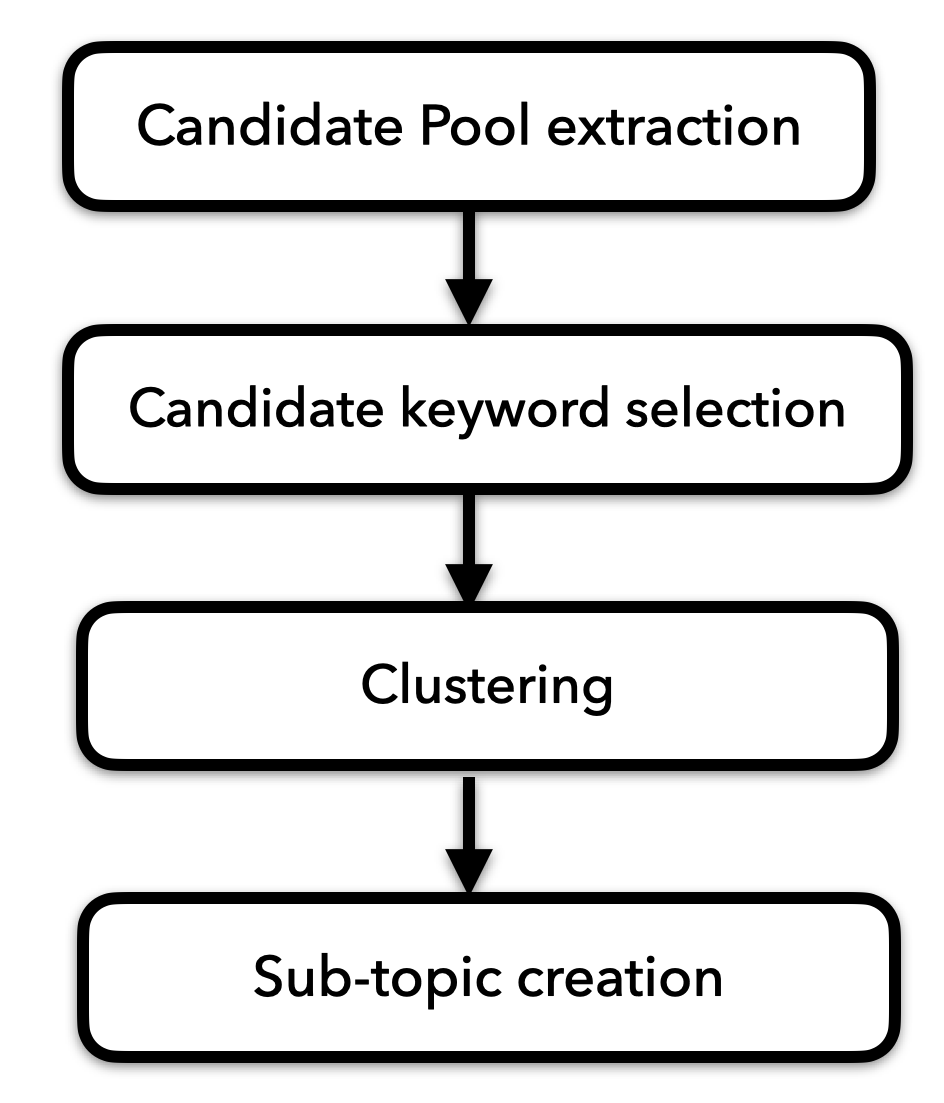
\includegraphics[width=.35\textwidth]{images/thesis_images/methodology.png}
	\caption{Proposed approach on an abstract level. \label{fig:methodology2}}
\end{figure}

The proposed approach, shown in \prettyref{fig:methodology2}, does not assume fixed templates or specific user intentions. The major components in the pipeline are: \emph{Candidate pool selection, Noun chunk extraction, Automatic keyword extraction, Candidate keyword selection, Clustering, and Sub-topic creation}. The first step of this pipeline is to retrieve a candidate or retrieval pool for the given query. Subsequently, a candidate selection module is proposed to extract keywords with high diversity and low noise (stopwords). This component consists of three significant steps, namely \emph{Noun chunk extraction, Automatic keyword extraction, and Candidate keyword selection}. Automatic keyword extraction involves extracting the most meaningful noun phrases in a text document. Specific keywords are selected and used for clustering using a percentile selection technique. This process is referred to as candidate keyword selection, and the resulting phrases after this stage are called candidate keywords. The following sections provide a detailed explanation of the above pipeline.




\section{Candidate Pool Selection}


A large set of retrieved documents for the query is required for a wide variety of these sub-topics. This set is referred to as the \emph{Candidate pool} and comprises retrieved results from both semantic and lexical matching. \prettyref{fig:candidate_pool} depicts the generation of the candidate pool from the document indices. A diverse and large candidate pool is crucial for generating a wide variety of query-related sub-topics. The length of a candidate pool directly influences the output of sub-topics, and two candidate pools of lengths around 30 and 100 are considered in this approach. These document pools are constructed from an equal mixture of documents retrieved from lexical and semantic matching.


\begin{figure}[h]
	\centering
	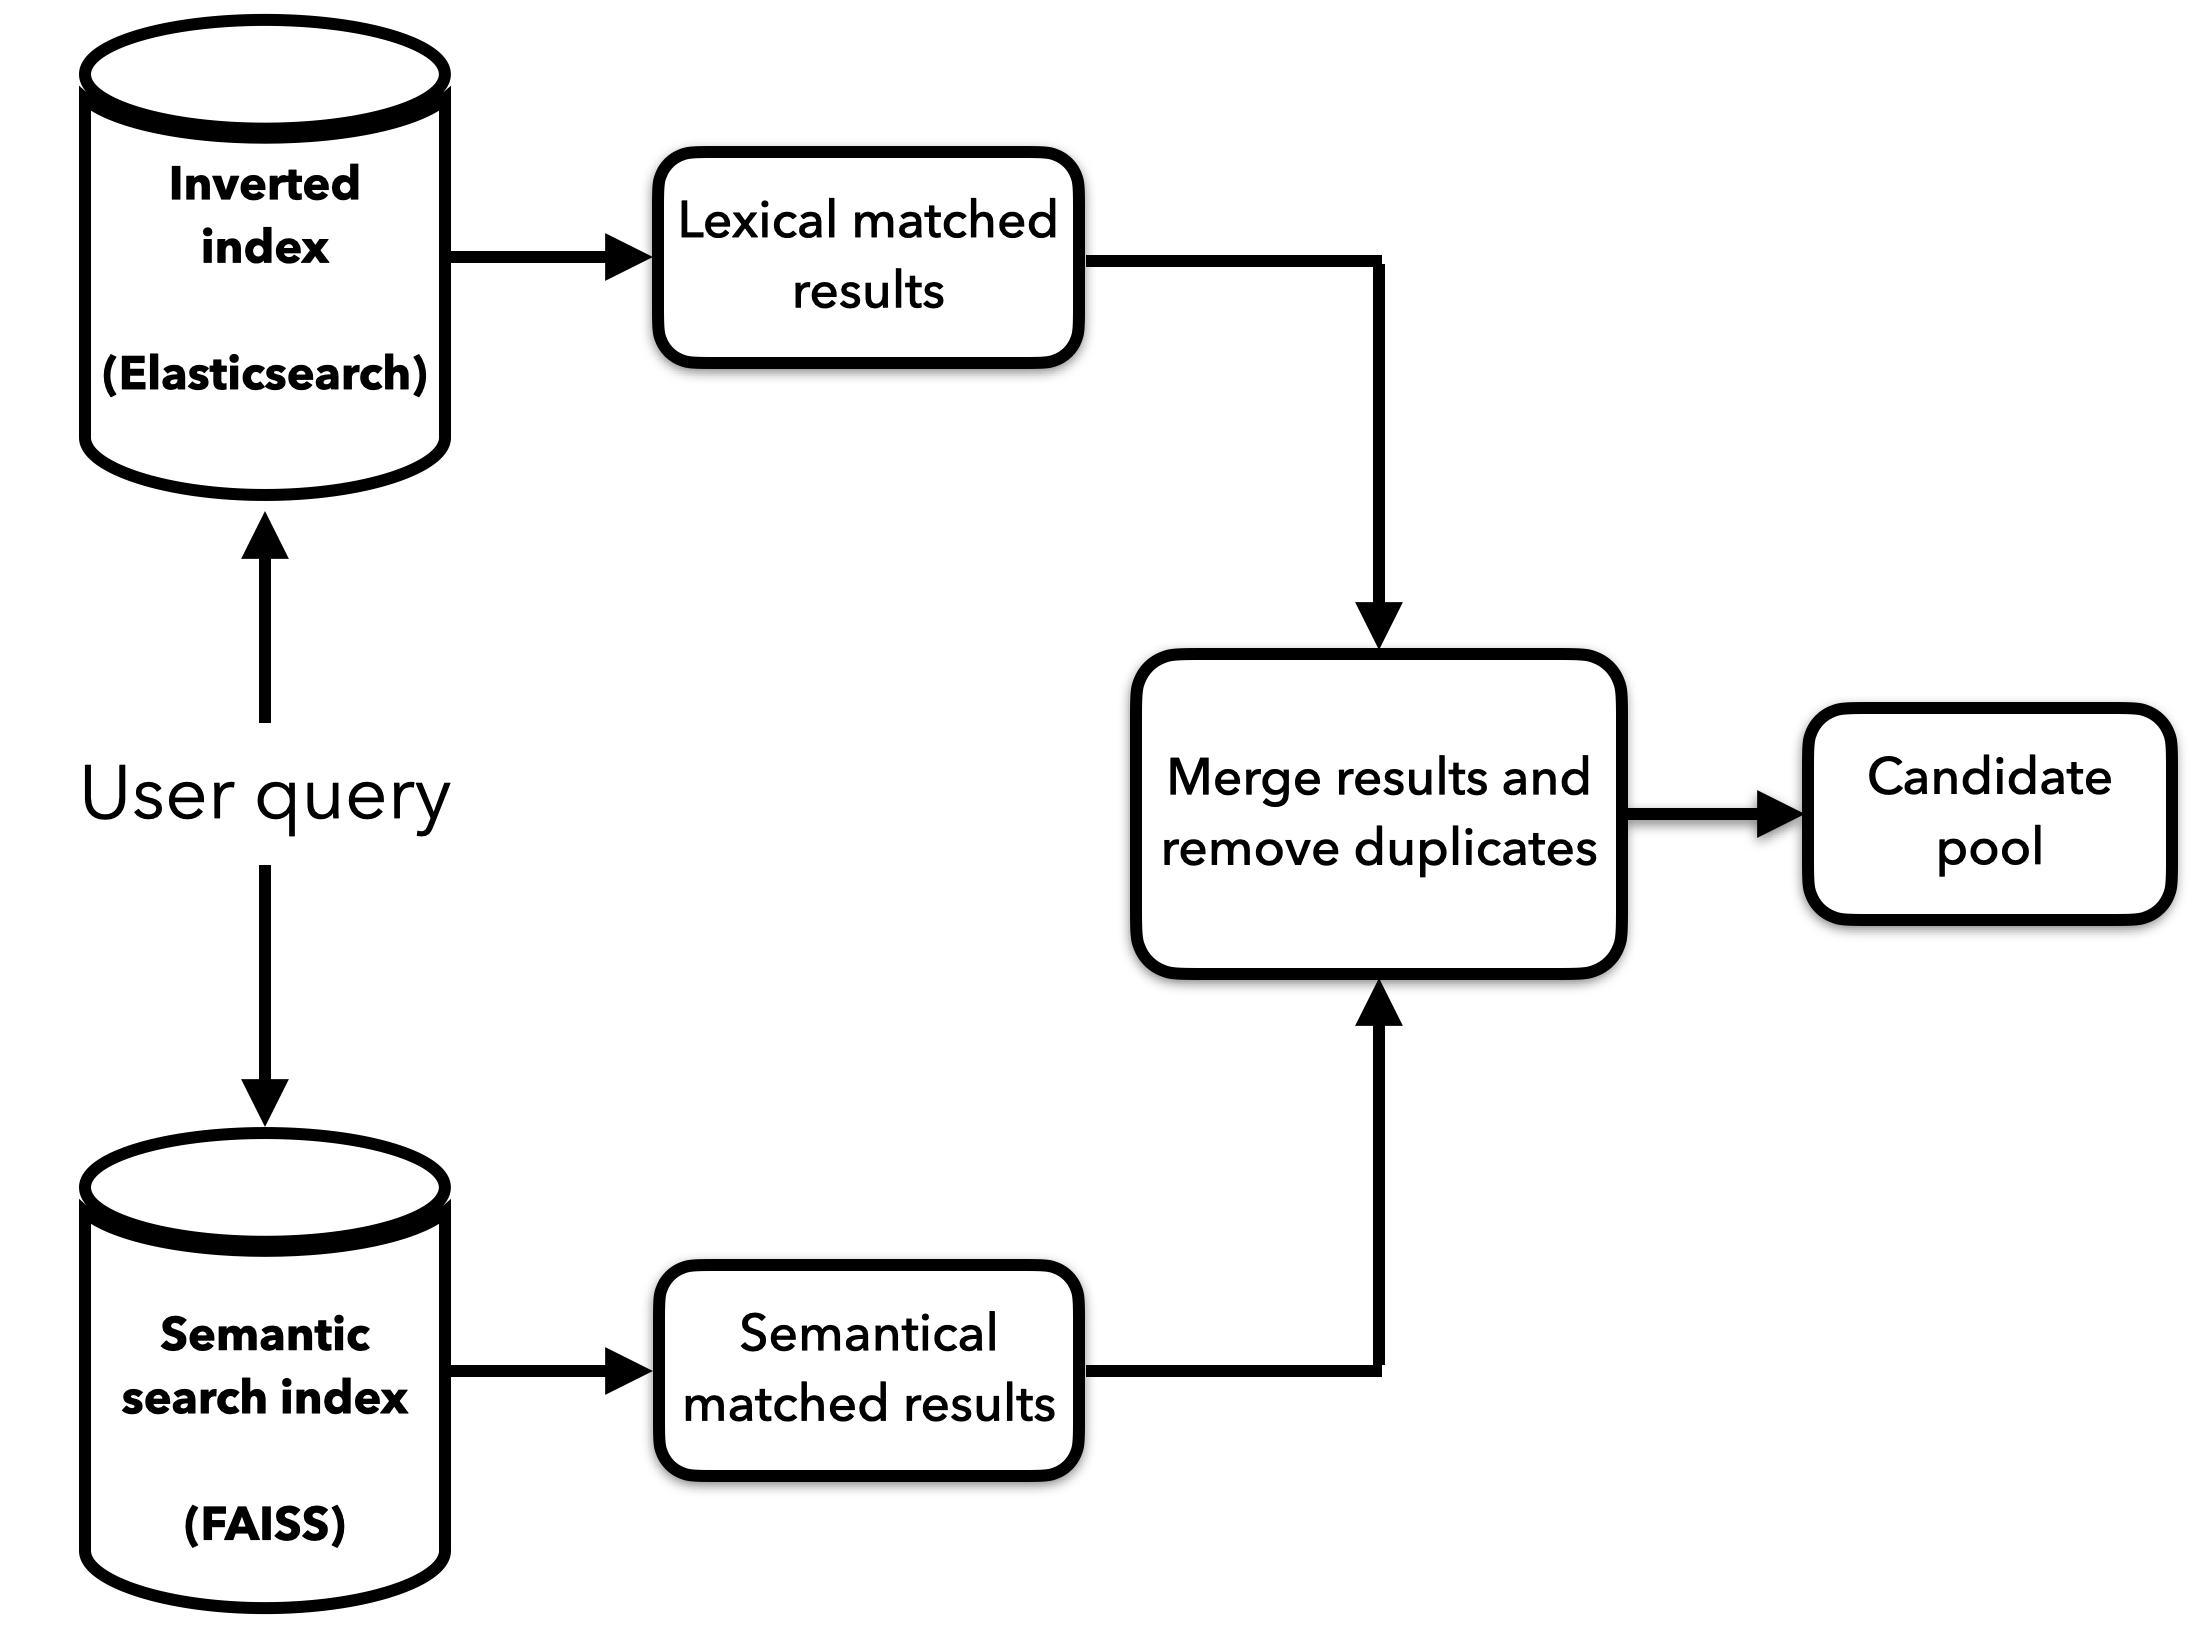
\includegraphics[width=.8\textwidth]{images/thesis_images/candidate_pool.png}
	\caption{Steps to generate a diverse candidate document pool.  \label{fig:candidate_pool}}
\end{figure}

\mycomment{\begin{algorithm}[H]
		\SetKwInput{KwInput}{Input}                % Set the Input
		\SetKwInput{KwOutput}{Output}              % set the Output
		\DontPrintSemicolon
		
		\KwInput{query - string, pool\_size - integer}
		\KwOutput{candidate\_pool - list $[candidate\_pool\_i]$, $i=1, 2, \cdots, n$, where each element is a string}
		% \KwData{Testing set $x$}
		
		% Set Function Names
		\SetKwFunction{FGetcandidate}{Get\_candidate\_pool}
		
		
		% Write Function with word ``Function''
		\SetKwProg{Fn}{Function}{:}{}
		\Fn{\FGetcandidate{$query$, $pool\_size$}}{
			
			\;
			pool\_size\_half = int(pool\_size/2)\;
			\;
			
			\tcc{get\_elastic\_search\_results -  retrieves documents which have high lexical similarity with the query.}
			
			top\_docs\_lexical = get\_elastic\_search\_results (query,  pool\_size\_half)\;
			
			\;
			\tcc{get\_semantic\_matching\_results - retrieves documents which have high semantic similarity with the query.}
			
			top\_docs\_semantic = get\_semantic\_matching\_results (query,  pool\_size\_half)\;
			\;
			
			\tcc{removes common documents which are present in both sets}
			candidate\_pool = remove\_duplicates (top\_docs\_lexical + top\_docs\_semantic)\;
			\;
			
			\KwRet candidate\_pool\;
		}
		\caption{Generate candidate document pool.}
\end{algorithm}}

It is assumed that the top retrieved documents are relevant to the query and the user, and thus, these retrieved documents are used for sub-topic extraction. This assumption can lead to poor sub-topics when the retrieved documents are entirely unrelated to the query, especially in the case of semantic matching. In lexical matching, the retrieved documents contain the query keywords and ensure that the documents are at least partially relevant. However, only cosine similarity is used as the selection criteria in semantic matching. For example, to create a \textit{\ac{CP} of 30} (\ac{CP}-30), top 15 documents from lexical matching results and top 15 documents from semantic matching results are combined. There is a clear possibility that top semantically matched results are not entirely related to the user-given query. Consequently, the cosine similarity of these top semantically matched results needs to be evaluated before creating the candidate pool.

 
 \begin{figure}[h]
 	\centering
 	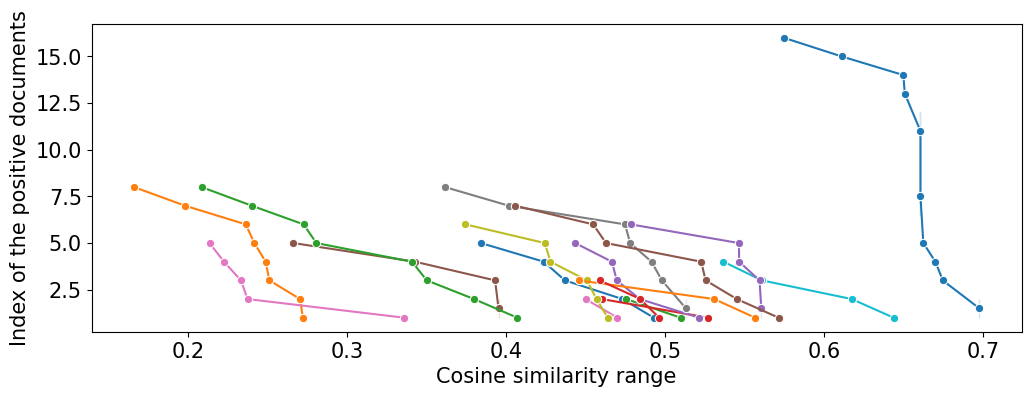
\includegraphics[width=.95\textwidth]{images/results/candidate_pool_analysis.png}
 	\caption[Cosine similarity distribution.]{Cosine similarity between the query and retrieved documents. \label{fig:cosine_sim_range}}
 \end{figure}
 
The cosine similarities between the query and retrieved documents are closely observed to perform this analysis. In the retrieved documents, only relevant documents and the document with the highest cosine similarity are considered. In \prettyref{fig:cosine_sim_range}, each query is shown in a unique colored plot, and it is clear that the spread of cosine similarity differs from query to query. Queries have high cosine similarities with the retrieved results ranging from 0.5, and some queries even have a range up to 0.7. On the other hand, there are some queries with a cosine similarity range below 0.3. Considering the maximum \emph{\ac{CS}} in the retrieved documents ($CS_{\mathrm{max}}$) as the reference, an appropriate lower similarity threshold ($CS_{\mathrm{min}}$) needs to be determined so that only an optimal set of retrieved documents is selected for the candidate pool. This information is represented in the equation below with the help of a cutoff parameter $cp$.
 \\
 
 	\centerline{$CS_{\mathrm{min}}$ = $( cp * CS_{\mathrm{max}} )$}
 	
 	
From the above equation, the value of $cp$ can be determined in multiple ways. One approach tested in this master thesis is the average min-max similarity ratio. The ratio is calculated from the mean of the minimum to maximum cosine similarities over multiple queries. Let us consider the maximum cosine similarity in the retrieved results set of query $q$ as $ max_{\mathrm{q}}$, and the minimum cosine similarity of the relevant document as $ min_{\mathrm{q}}$. Now the approximation of the value $cp$ over $N$ queries is described as:

 
  	\centerline{$cp$ = $( \sum\limits_{q=1}^N  min_{\mathrm{q}}/ max_{\mathrm{q}}) /N$}
 
Applying the above approximation to the data from \prettyref{fig:cosine_sim_range} resulted in the value of $cp$ = 0.78. However, a slightly lower value of 0.75 is chosen in the end, as there may be an expected human bias during data labeling. Multiple labelers are involved in labeling the documents for different queries, and this can lead to possible deviation from the true value. This optimal threshold selection is designed to prevent the selection of irrelevant documents for a given user query. This selection technique can be employed in any semantic matching \ac{IR}.

 

\begin{algorithm}[H]
	\SetKwInput{KwInput}{Input}                % Set the Input
	\SetKwInput{KwOutput}{Output}              % set the Output
	\DontPrintSemicolon
	
	\KwInput{query - string, pool\_size - integer}
	\KwOutput{top\_docs\_semantic - list $[top\_docs\_semantic\_i]$, $i=1, 2, \cdots, n$, where each element is a string}
	% \KwData{Testing set $x$}
	
	% Set Function Names

	\SetKwFunction{FGetsemantic}{Get\_semantic\_matching\_results}
	
	
	% Write Function with word ``Function''
	\SetKwProg{Fn}{Function}{:}{}
	\Fn{\FGetsemantic{$query$, $pool\_size$}}{
		\;
		MIN\_THRESHOLD\_SEMANTIC = 0.27\;
		CP = 0.75\;
		\;
		
		\tcc{top\_docs\_semantic\_search - contains semantically similar documents, doc\_sim\_list - contains respective cosine similarity score}
		
		top\_docs\_semantic\_search, doc\_sim\_list = get\_semantic\_search\_results (query, pool\_size)\;
		\;
		max\_cosine\_sim = max (doc\_sim\_list)\;
		min\_cosine\_sim = min (doc\_sim\_list)\;
		max\_diff\_cosine\_sim = get\_max\_diff\_sim (doc\_sim\_list)\;

		\;
		\tcc{Optimal cutoff similarity selection from three individual cutoffs}
		final\_cutoff\_sim = min (MIN\_THRESHOLD\_SEMANTIC, (CP * max\_cosine\_sim), max\_diff\_cosine\_sim)\;
		\;
		
		top\_docs\_semantic = []\;
		
		
		\For{$idx\gets0$ \KwTo $pool\_size$}{
			\;
			doc = top\_docs\_semantic\_search[$idx$]\;
			sim = doc\_sim\_list[$idx$]\;
			
			\tcp{Selecting documents that have high cosine similarty than the optimal cutoff similarity.}
			\If{sim > final\_cutoff\_sim}
			{
				top\_document\_semantic.append(doc)\;
			}

		}
		\;
		
		
		\If{len (top\_docs\_semantic) < 10}
		{
			\tcc{Selecting only top 10 in case of poor similarity distribution between the query and documents}
		top\_docs\_semantic = top\_docs\_semantic\_search[:10]\;
		}
		\;

		 	\caption{Retrieve semantically similar documents with optimal selection.} \label{algo:optimal_selection}
		\KwRet top\_docs\_semantic\;
	}
	
\end{algorithm}


Furthermore, it is also observed that some queries exhibit abnormal cosine similarity distributions, such as cosine similarity values below 0.3 as shown in \prettyref{fig:cosine_sim_range}. An optimal candidate pool selection approach is proposed to handle these exceptional cases. This technique extends the existing threshold by considering two additional criteria. These criteria are chosen in the context of unexpected or poor query-to-document distributions. The first criterion establishes a fixed threshold for cosine similarity, while the second criterion captures the maximum difference in cosine similarity between the top two similar documents.

 Algorithms \prettyref{algo:optimal_selection} and \prettyref{algo:max_diff} further detail these criteria. In the case of no results at the end of the selection, the top 10 semantically matched documents are chosen. After the successful selection of documents from semantic matching, the documents from lexical matching are combined and duplicates are removed. The resulting set of documents without any redundancy is then referred to as the candidate pool.

 
 \begin{algorithm}[H]
 	\SetKwInput{KwInput}{Input}                % Set the Input
 	\SetKwInput{KwOutput}{Output}              % set the Output
 	\DontPrintSemicolon
 	
 	\KwInput{sim\_list - list $[sim\_list\_i]$, $i=1, 2, \cdots, n$, where each element is a float }
 	\KwOutput{max\_diff\_sim - float}
 	% \KwData{Testing set $x$}
 	
 	% Set Function Names
 	\SetKwFunction{FMaxdiffsim}{Get\_max\_diff\_sim}
 	
 	% Write Function with word ``Function''
 	\SetKwProg{Fn}{Function}{:}{}
 	\Fn{\FMaxdiffsim{$sim\_list$}}{
 		
 		\;
 		diff\_list = []\;
 		sim\_list\_len = len(sim\_list)\;
 		\;
 		
 		\For{$idx\gets1$ \KwTo $sim\_list\_len$}{
 			\tcp{store the difference in similarities at recurrent indices.}
 			diff\_list.append(sim\_list [$idx$] - sim\_list [$idx$ - 1])
 		}
 		\;
 		
 		max\_diff = max(diff\_list)\;
 		\tcp{Get the index where the similarity difference is maximum.}
 		max\_diff\_index =  diff\_list.index(max\_diff)\;
 		\;
 		
 		max\_diff\_sim = sim\_list[max\_diff\_index]\;
 		\;
 		\KwRet max\_diff\_sim\;
 	}
 	
 	\caption{Calculate similarity at the maximum difference.} \label{algo:max_diff}
 \end{algorithm}

\section{Candidate Keyword Selection}

This section details the steps involved in selecting specific keywords and the criteria involved
in their selection. The main objective of this stage is to choose highly diverse noun chunks from each
text document. Candidate keyword selection is the most crucial step in the entire pipeline, and the
quality of the clustering output directly depends on the outcome of this step.

\subsection{Noun Chunk Extraction}

News articles are very long text documents and nouns serve as essential parts of speech elements that identify people, places, or things. A noun chunk is a phrase (a group of words) that represents a noun. To automatically extract the noun chunks from each document, a library named \emph{spacy}\footnote{\url{https://spacy.io/}} is used. The noun chunks from spacy are closely analyzed, and some inconsistencies are identified that require further cleaning. A unique pipeline is proposed to clean these noun chunks, targeting the noise elements: stopwords, punctuation, determiners, duplicates, and long noun chunks.

 
 \begin{description}
 	\item[Remove longer Noun chunks] \hfill \\  It has been observed in the output of spacy noun chunks that there are some  noun phrases consisting of more than three words, which mostly lack significant information. Consequently, these noun chunks are removed from the spacy output. For example, in German, the phrase \emph{"standort- und zeitunabhängigen Zusammenarbeit"} and in English, the phrase \emph{"Every successive cellular generation"}. Although there might be useful information within these long noun phrases, extracting that information is very challenging. The occurrence ratio of these phrases is relatively smaller compared to phrases with a length below 3. Therefore, these long noun phrases are filtered out from the set of noun chunks.
 	
 	\item[Remove stopwords] \hfill \\  Stopwords are words that carry no significant information and are thus omitted from the noun chunks. There is no universal set of stopwords in any language, and there are also numerous types of stopwords observed in news articles in both English and German languages. Therefore, a robust set of stopwords from various sources\footnote{\url{https://gist.github.com/sebleier/554280, https://countwordsfree.com/stopwords, https://solariz.de/de/downloads/6/german-enhanced-stopwords.htm}} has been collected in both languages. Stopwords can appear either as a complete noun chunk or as part of a noun chunk, and they are removed in either case. Stopwords generally consist of determiners, adjectives, articles, prepositions, etc.
 	
 	
 	\item[Remove numeric noun chunks] \hfill \\  Some noun chunks have numeric values that contain no useful information, and furthermore, it is observed that the complete noun chunk does not convey any significance either. Thus, the numeric noun chunks are removed from the noun chunks set. For example, \emph{"mehr als 50 Ländern", "1,95 m Länge", "1,5 Milliarden"} in German, etc. However, the noun chunks where the numeric value is attached to an alphabet are ignored, i.e., \emph{"4G Technology", "3D designs"} in English, etc.
 	
 	
 	\item[Remove punctuation]  \hfill \\ This step is designed to remove all sorts of punctuation elements and keep the noun chunks clean and more readable to the user. For example, the original noun chunk "Bündnis- und Landesverteidigung" is transformed to \emph{"Bündnis Landesverteidigung"} after removing the hyphen (-) and the stopword (und).
 	
 	
 	\item[Lemmatization] \hfill \\  Lemmatization is the process of extracting the base or normalized form from the original words~\cite{plisson2004rule}. For example, 'worse' and 'worst' are lemmatized to their base form 'bad'. Lemmatization helps text processing techniques based on lexical matching and reduces computational and storage complexity. In this thesis, lemmatization is performed with the help of spacy library for both the English and German languages.
 	
 	
 	\item[Fuzzy redundancy removal] \hfill \\  It is observed that there are a lot of noun chunks that are syntactically similar to each other. These similar noun chunks can be categorized into two types, namely exact duplicates and close duplicates. Exact duplicate noun chunks can be easily filtered in Python, but identifying the close duplicates and filtering is a challenge. For example, the noun chunks "5G network" and "5G 4G network". 
 	
 	Only one of the noun chunks i.e. longer noun chunk is retained, and the other is removed. Algorithm \prettyref{algo:close_duplicates} details the steps used to achieve the cleaned noun chunks. The main objective of this step is to reduce the similar phrases and increase diversity in the data. This can lead to a loss of information to a certain extent. Accordingly, a fuzzy string matching-based noun chunk removal approach is designed to tackle the above problem, and close duplicates are removed to a certain extent using the FuzzyWuzzy library (refer to Appendix \ref{appendix:A} for more information).
 	
 	
 \end{description}

 	
 	\begin{algorithm}[H]
	\SetKwInput{KwInput}{Input}                % Set the Input
	\SetKwInput{KwOutput}{Output}              % set the Output
	\DontPrintSemicolon
	
	\KwInput{noun\_chunk\_list - list $[noun\_chunk\_list\_i]$, $i=1, 2, \cdots, n$, where each element is a string }
	\KwOutput{cleaned\_noun\_chunk\_list - list $[cleaned\_noun\_chunk\_list\_i]$, $i=1, 2, \cdots, n$, where each element is a string }
	% \KwData{Testing set $x$}
	
	% Set Function Names
	\SetKwFunction{FRemovdup}{Remove\_close\_duplicates}
	
	% Write Function with word ``Function''
	\SetKwProg{Fn}{Function}{:}{}
	\Fn{\FRemovdup{$noun\_chunk\_list$}}{
		
		\;
		\tcp{Removing exact duplicates using set in python}
		noun\_chunk\_list = list(set(noun\_chunk\_list))\;
		
		
		\;
		close\_duplicates = []\;
		noun\_chunk\_list\_len = len(noun\_chunk\_list)\;
		
		\;
		
		\For{$i\gets1$ \KwTo $noun\_chunk\_list\_len$}{
			
			phrase\_1 = noun\_chunk\_list [$i$]\;
			\;
			
			\For{$j\gets i+1$ \KwTo $noun\_chunk\_list\_len$}{
				
				phrase\_2 = noun\_chunk\_list [$j$]\;
				\;
				
				\tcp{fuzzy gives the syntactical text similarity score}
				\If{fuzzy (phrase\_1, phrase\_2) > 85}
				{
					
					\tcp{When the score is high, the smaller phrase is recorded}
					
					close\_duplicates.append(get\_shorter\_text(phrase\_1, phrase\_2))\;
				}
				\;
				
				
			}
			\;
			
		}
		
		\tcp{Removing the close duplicates using recorded close\_duplicates}
		cleaned\_noun\_chunk\_list = list(set(noun\_chunk\_list) - set(close\_duplicates))\;
		\;
		\KwRet cleaned\_noun\_chunk\_list\;
	}
	
	\caption{Algorithm to remove close duplicates.} \label{algo:close_duplicates}
\end{algorithm}


\subsection{Keyword Extraction}
The cleaned noun chunks describe a text document very well. However, not all noun chunks are of great significance in representing a document, especially in the case of a news article. As the length of the news article is large, the size of the extracted noun chunk set can also be large. This large set of noun chunks is well-processed syntactically. It needs to be processed now semantically to select only noun chunks that can significantly influence the meaning of a text document (a news article). These crucial noun chunks in a text document are referred to as \textit{Keywords}.


Transformer architectures compute context-aware embeddings of tokens in a sentence, considering the order and identity of the tokens. These token-level representations are further averaged to calculate sentence embeddings. However, using sentence-level embeddings as the mean of token embeddings can result in poor representations of long text documents. In news articles, it is observed that the length of the text documents is longer, and different contexts are discussed in different paragraphs. Therefore, the document is divided into multiple paragraphs, and the mean of all paragraph embeddings is considered as a "Document representation vector". In this approach, a paragraph length of 500 tokens is considered. For example, a text document with a token length of 1600 is divided into four paragraphs of lengths 500, 500, 500, and 100, respectively. The final document representation vector is the mean representation vector of these paragraph vectors. The best possible parameter for the paragraph length is not explicitly tested in this master thesis and can be considered as future work.



\begin{figure}[h]
	\centering
	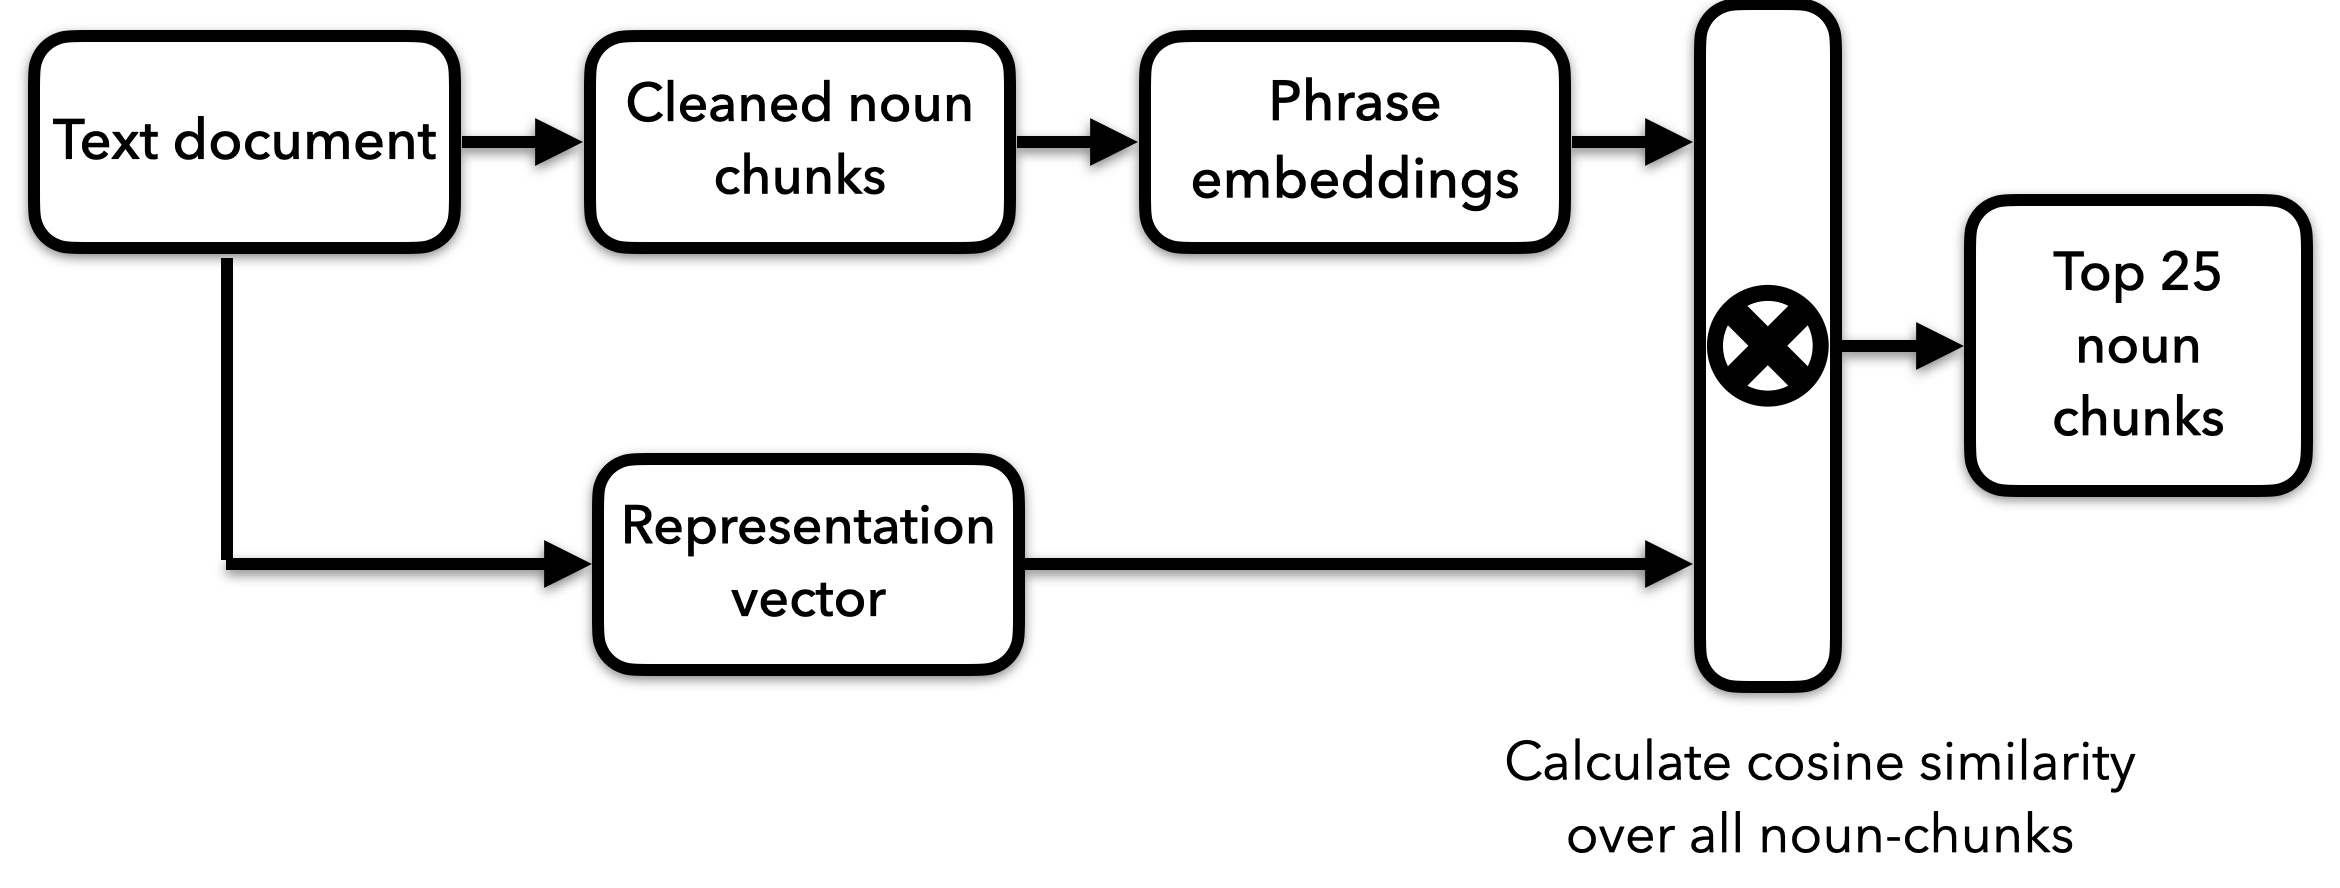
\includegraphics[width=.9\textwidth]{images/thesis_images/keyword_extraction.png}
	\caption[Contextualized automatic keyword extraction.]{Automatic keyword extraction using phrase embeddings. \label{fig:keyword_extraction}}
\end{figure}


Phrase embeddings are semantic representations of noun chunks that are computed using the \ac{USE} model. By utilizing noun chunk embeddings and the document representation vector, the relevance of a noun chunk in a document is expressed as the cosine similarity between the vectors in the semantic space. The higher the similarity, the greater the relevance of the noun chunk in the document. Consequently, all noun chunks are ranked according to their similarity of relevance with the document. The top 25 noun chunks with the highest relevance similarity are considered as "Keywords". The pipeline for extracting these keywords is shown in \prettyref{fig:keyword_extraction}.


\subsection{Candidate Keyword Selection}


Keywords extracted from a document in the earlier stage are syntactically diverse, as they are derived from the noun chunks generated by removing the close duplicates. Let us consider the case of using these keywords to distinguish documents in an \ac{IR} setup, where the user provides a search query and expects relevant documents. Through preliminary manual analysis, it has been observed that there are certain keywords that are dissimilar to the user query but hold significant value in improving the information search behavior. Therefore, the task of removing the query-related keywords and retaining the highly distinctive keywords is referred to as \emph{Candidate keyword selection}.


Let us consider a text corpus $C$ that contains $n$ documents, where each document $D$ is a news article. These documents are stored in two indices, namely the inverted index and the semantic search indices, for retrieving documents based on a given search query.


\centerline{$C$ = $\{D_1, D_2, D_3,\dots, D_n\}$}

Once the user provides the IR system a search query $q$ and a candidate pool $CP$ of size $m$ is generated, which is a document set.

\centerline{$CP_q$ = $\{D_i, D_j, D_k,\dots\}$}


Taking one document $D_i$ into account, a set of keywords ($k$) is extracted using the above steps, namely noun chunking and automatic keyword extraction. The news article is then transformed into a group of keywords, as expressed below.


\centerline{$D_i$ = $\{k_1, k_2, k_3,\dots\}$ } 

The objective of this step is to efficiently select specific keywords that are similar to the query. This selection process also takes into consideration the close semantic and multi-lingual nature of the keywords. To achieve this, cosine similarity is utilized, and the multi-lingual \ac{USE} model is employed to encode both the query and the keywords into semantic embeddings. The similarity between the query and the document keywords is determined by the distance in the semantic space. Keywords with low cosine similarity are selected to ensure a diverse range of keywords in relation to the query. To remove keywords that are similar to the query, a parameter called candidate keyword selection ($cks$) parameter is proposed.

The selection parameter considers the distribution of similarity between the query and keywords within a document. Furthermore, it should be independent of any specific document. A percentile selection criterion is adopted to avoid using a static similarity threshold. The similarity score of the $x$ percentile indicates that the score is higher than $x$ percent of the population or the similarity is lower than $100-x$ percent of the population. In the case of $cks$-based selection, only the keywords that are not similar to the query are of interest, and are therefore selected. For example, $cks$ = 60 denotes the selection of keywords with query similarity less than the 60th percentile similarity and the removal of keywords higher than the 60th percentile. Similarly, a value of $cks$ = 100 represents the selection of all keywords without any removal. 

The keywords selected as the outcome of candidate keyword selection are referred to as "Candidate keywords". After candidate keyword selection process for a given user query $q$, one document  or news article $D_i$ can be represented as a set of candidate keywords $ck$. Notably, candidate keywords are a subset of keywords.


\centerline{$D_i$ = $\{ck_1, ck_2, ck_3,\dots\}$ } 


The keyword selection for a given $cks$ parameter is illustrated in \prettyref{tab:cks_selection}. As far as my knowledge goes, this selective approach to improving clustering and \ac{IR} performance is one of the earliest attempts in \ac{IR} system research. Additional criteria for enhanced keyword selection, beyond query similarity, should be further explored in the future work.

\begin{center}
	\captionof{table}{Different $cks$ parameter examples.}\label{tab:cks_selection}
	\begin{tabularx}{.9\textwidth}{|c|Y|}
		\hline
		Cks parameter  &  Selected candidate keywords  \\
		\hline
		
		\textbf{100}  &            All keywords   \\ \hline
		75 &            Keywords with query similarity lower than 75th percentile  \\ \hline
		50 &            Keywords with query similarity lower than 50th percentile  \\ \hline
		25 &            Keywords with query similarity lower than 25th percentile   \\ \hline
		10 &            Keywords with query similarity lower than 10th percentile \\ \hline
		
	\end{tabularx}
	
\end{center}



\section{Keyword Clustering}

Candidate keywords from each document in the candidate pool are combined, and duplicates are removed to create a final set of candidate keywords. The combined candidate keywords set from all news articles in the candidate pool for a query $q$ is represented as $M_q$. These keywords are further clustered using the \ac{HDBSCAN} algorithm to generate distinctive sub-topics. This stage has three main steps, namely \emph{Phrase embeddings extraction}, \emph{Dimensionality reduction}, and \emph{Hierarchical clustering}. 

To achieve semantic clustering, multi-lingual \ac{USE} model are used to generate phrase embeddings for each candidate keyword. These densely distributed embeddings are usually highly dimensional (512), and clustering in high-dimensional space is complex to capture patterns and can be resource-intensive. Therefore, the embeddings are compressed with the help of a dimensionality reduction technique, namely \ac{UMAP}. The dimensionality of the embeddings is reduced without losing underlying information in the data using the \ac{UMAP} algorithm~\cite{mcinnes2018umap} from the umap-learn\footnote{\url{https://pypi.org/project/umap-learn/}} library.

\begin{figure}[h]
	\centering
	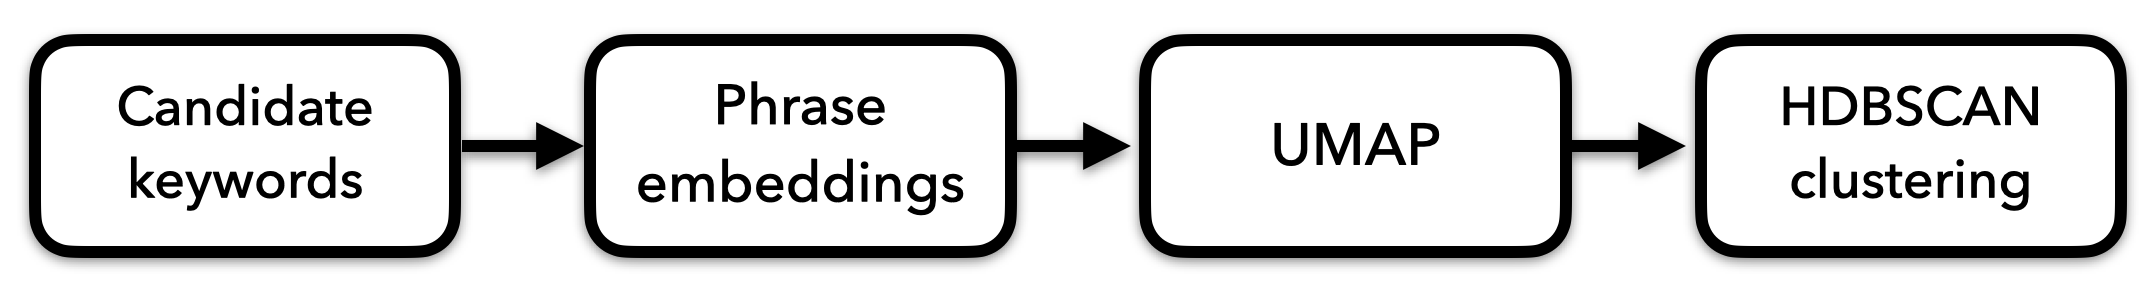
\includegraphics[width=.9\textwidth]{images/thesis_images/clustering.png}
	\caption{Clustering to generate sub-topics.  \label{fig:clustering}}
\end{figure}

 
These embeddings are further clustered in low dimensions using a hierarchical clustering algorithm. Noise is expected in the candidate keyword extraction phase, and not all keywords are crucial for modeling. Therefore, clustering algorithms such as k-means and gaussian mixture models are not suggested in this case, as they assign all data points to a cluster during clustering. Furthermore, these algorithms assume a specific cluster shape, either spherical or elliptical. Consequently, density-based algorithms like the \ac{HDBSCAN} clustering algorithm are preferred because they inherently account for noise in the data and prevent assigning a cluster to every data point.

One significant advantage of these algorithms is that the number of clusters is not a parameter, and the algorithm effectively creates clusters based on the data. The \ac{HDBSCAN} algorithm~\cite{mcinnes2017hdbscan}, with its varying epsilon and merging clusters, has shown robust clustering results by finding clusters with varying densities. The same algorithm is considered in this master's thesis. \prettyref{fig:clustering} presents the steps taken to perform clustering after extracting the candidate keywords. This clustering pipeline has already been tested and has shown excellent results with documents in recent research~\cite{angelov2020top2vec}. However, in this approach, keywords are clustered rather than the documents, and later the keywords and documents are connected using "sub-topics".




\section{Sub-topic Creation} 

After clustering, sub-topics are extracted using a centroid approach. A mean phrase vector (centroid vector) is calculated from all the keywords inside a cluster, and the closest keyword vector to the centroid vector is considered a cluster label. This process is named \textit{Cluster labeling}, and the cluster labels are considered as "Sub-topics". Sub-topics and documents inside a sub-topic can be further ranked before showing them to the user. The pipeline ends with this last component, \emph{Sub-topic creation}.  The phrases "sub-topic modeling" or "sub-topic clustering" are identical to the outcome of complete pipeline. The code developed for the complete sub-topic retrieval and testing is shared in the GitHub repository \textit{Sub-topic-retrieval-thesis}\footnote{\url{https://github.com/praveengadiyaram369/Sub-topic-retrieval-thesis}}.


Thereafter the candidate keyword set $M_q$ is clustered into $r$ groups ($s$) and is defined as a sub-topic set $S_q$. 

\centerline{$S_q$ = $\{s_i, s_j, s_k,\dots, s_r\}$}

Each sub-topic ($s$) is again expressed as a set of candidate keywords  ($ck$). The number of candidate keywords in a sub-topic cluster can vary from cluster to cluster.

\centerline{$s_i$ = $\{ck_x, ck_y, ck_z,\dots\}$}

The mapping between the document and keywords has already been established above. Now, each document can be expressed as a set of sub-topics, where each sub-topic is further described as a set of documents. Candidate keywords serve as the foundational concepts for the modeling relationship between the sub-topics and documents.

\centerline{$D_p$ = $\{s_i, s_j, s_k,\dots\}$ }
\centerline{$s_q$ = $\{D_x, D_y, D_z,\dots\}$}



    
        % !TEX root = ../thesis.tex

\chapter{Experiment Setup}

The experiment is divided into three parts in order to address the three research questions proposed in Section 1.2. In this chapter, everything needed to conduct the experiment, such as the testset, system specifications, hyperparameter selection, etc., is described in seven sections. The section \emph{Clustering evaluation} details the evaluation of clustering results and the selection of the best parameters for the proposed pipeline. Subsequently, the section \emph{Survey evaluation} illustrates the survey design, \ac{IR} system introduction, and comparison strategy. Finally, the section \emph{Precision evaluation} introduces the literature comparison and retrieval performance strategies.



	\section{System Specifications}

The experiment is carried out in two different systems according to the time taken to execute specific tasks. All the code development, exploratory analysis, and statistical testing are performed on an HP ELITEBOOK system with an AMD Ryzen 5 PRO 4650U processor, 16 GB of RAM, and 500 GB of disk space. Web scraping, \ac{IR} system hosting, data storage, clustering, and further benchmark testing are performed on a large \ac{VM} hosted at \ac{FKIE}. The technical specifications of the \ac{VM} are four processors CPU (Intel(R) Xeon(R) Gold 6136 CPU @ 3.00GHz), 48 GB RAM, and 370 GB disk space.
	
	
	\section{Testset Description}

For two main reasons, finding a dataset specific to this research problem is difficult in the current \ac{IR} data repositories. Firstly, the search query needs to be a phrase rather than a sentence. Furthermore, the documents need to be labeled with a specific intention rather than just coherence with the query. The interest at \ac{FKIE} is to retrieve the documents related to \emph{Innovation and Technology,} and a new testset is collected for this purpose. Below are a few specific areas of interest in news articles that describe the user intention: \emph{Innovation, Technology breakthroughs, Future products, Applied research, New procurement strategies,} and \emph{Artificial Intelligence}. These topics are also described as positive document characteristics because a document is considered positive when it is strongly related to any of the above-mentioned characteristics.


The strategy for testset collection is to consider documents from lexical and semantic matching. The results from both algorithms help find the diverse contexts related to the user query. Therefore, a candidate pool with a maximum length of 30 documents is considered. Fifteen lexical and semantic matching documents are combined into a merged set where duplicate documents are removed. Relevance labeling is the task of assigning an appropriate label to the retrieval results inside the candidate pool by multiple independent labelers. Every labeler has to assign a label coherent with the query and consider the \ac{FKIE} user's intention, i.e., coherence with the positive document characteristics mentioned above. Once the labeler assigns a particular label to a document, the labeled information is stored in an \emph{SQLite DB}.


\mycomment{

\begin{figure}[h]
	\centering
	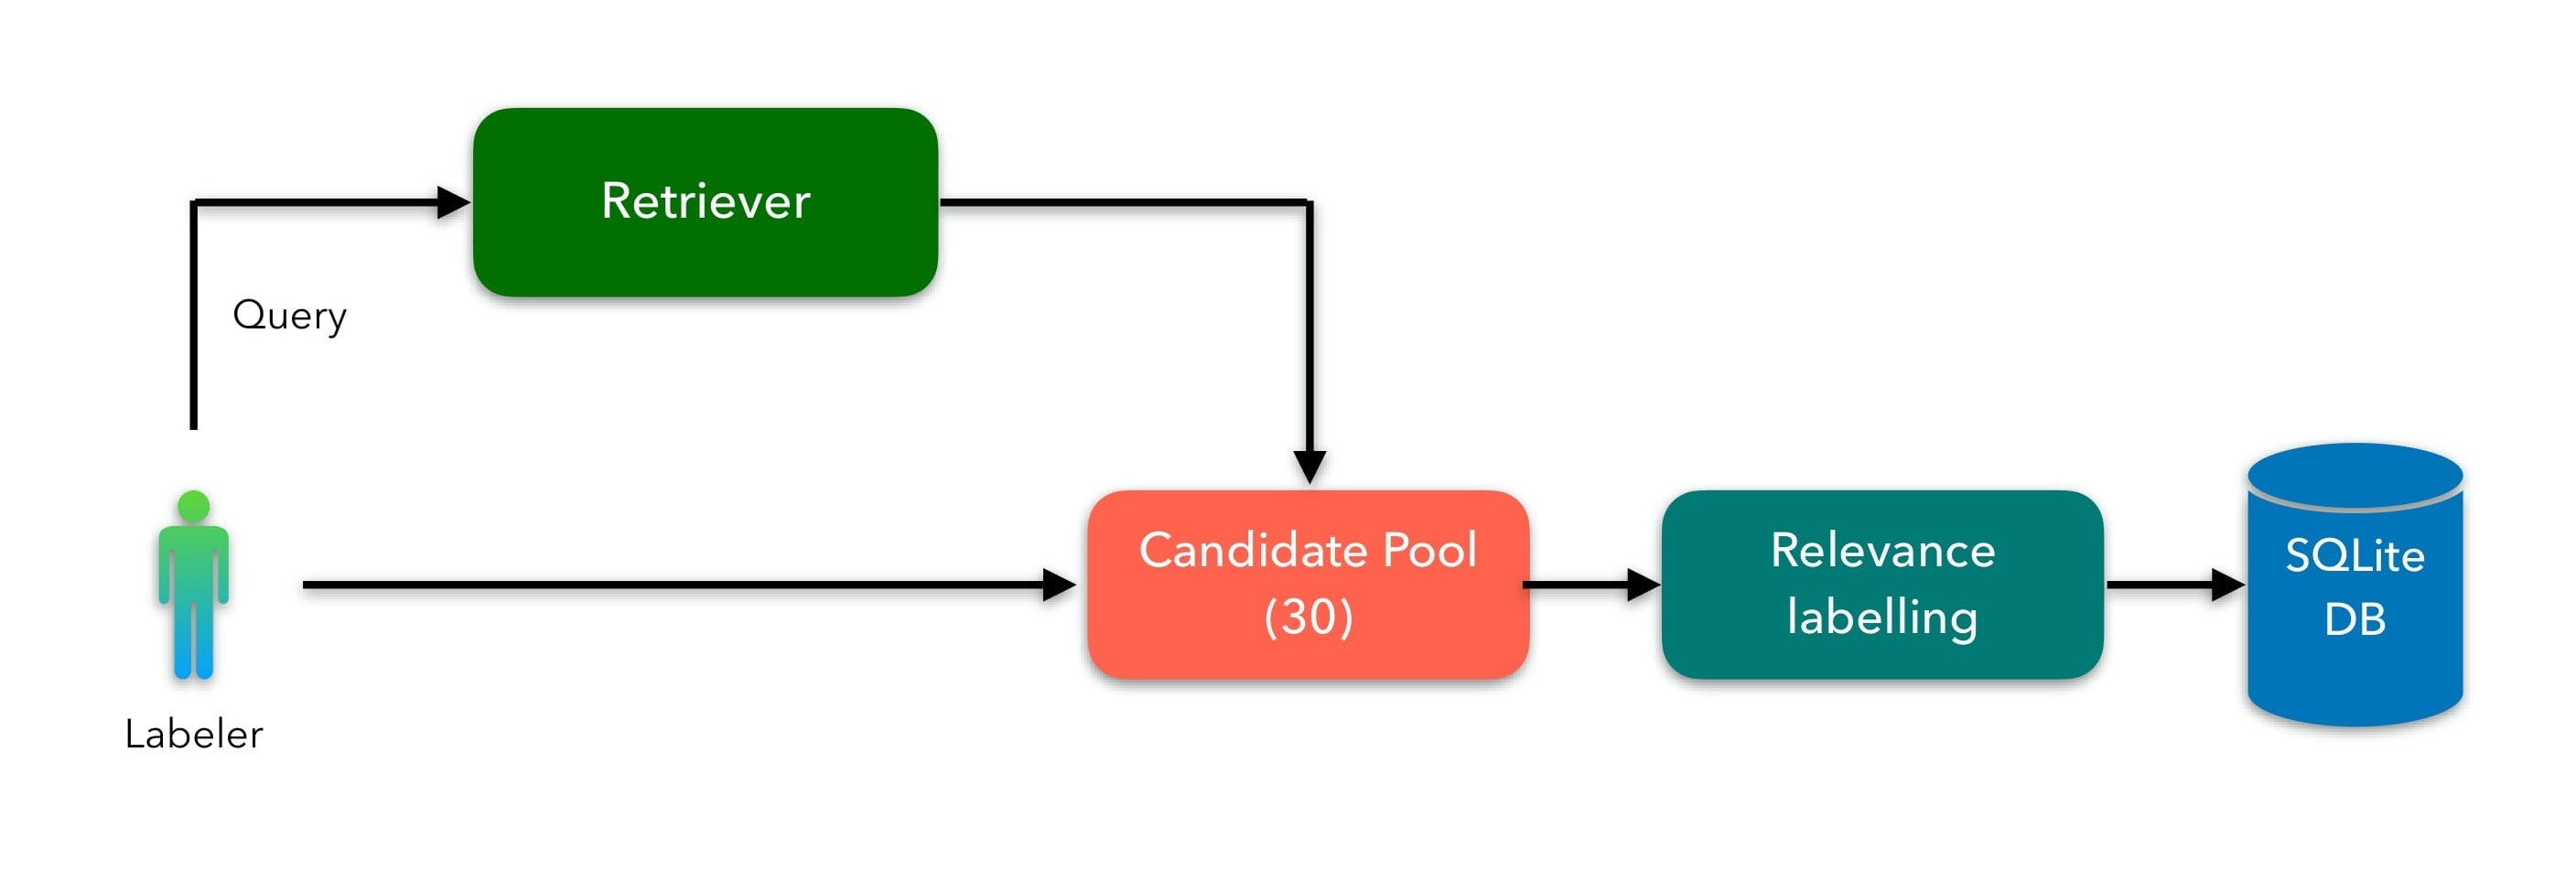
\includegraphics[width=.8\textwidth]{images/keynotes_images/dataset.jpg}
	\caption{Testset collection strategy. \label{fig:dataset}}
\end{figure}
}

\begin{center}
	\captionof{table}[Relevance labels introduction and details.]{Relevance labels definition and document distribution.}\label{tab:label_definitions}
	\begin{tabularx}{0.95\textwidth}{|c|c|c|Y|}
		\hline
		Label-id & Label name & Document count &  Label definition  \\
		\hline
		1 & Perfect & 78 & A document that closely aligns with one of the positive document characteristics. \\
		\hline
		2 & Partially relevant & 147 &  A document that contains keywords and seems to be relevant, yet still lacks innovation or novelty. \\
		\hline
		3 & Irrelevant & 306 & A document containing the given user keyword still lacks innovation and
		coherent discussion about the query. Eg: click-baits, advertisements, etc,. \\
		\hline
		4 & Wrong & 98 & These are false documents and unrelated to the user's query. \\
		\hline
	\end{tabularx}
\end{center}

A total of 22 queries are labeled by 5 different labelers. After analyzing the label distribution of the queries, it is observed that the distributions of perfect and partially relevant documents are very low compared to the other labels, as shown in \prettyref{tab:label_definitions}. For evaluation, 17 queries are considered and their respective label distributions are shown in \prettyref{tab:testset_queries}.

\begin{center}
	\captionof{table}{Testset queries used for the evaluation.}\label{tab:testset_queries}
\begin{tabularx}{0.95\textwidth}{|c|c|Y|Y|Y|Y|}
	\hline
	S No. & Query & Perfect & Partially relevant & Irrelevant & Wrong \\
	\hline
1	&  Architekturanalyse & 4 & 6 & 15 & 4 \\
	\hline
2	& Big Data, KI für Analyse	 & 7 & 11 & 10 & 2 \\
	\hline
3	& Edge computing & 1 & 5 & 11 & 11 \\
	\hline
4	& IT-Standards & 1 & 7 & 9 & 11 \\
	\hline
5	&  Kommunikationsnetze & 4 & 5 & 18 & 1 \\
	\hline
6	& Methode Architektur & 4 & 8 &  15 & 2 \\
	\hline
7	& Militärische Kommunikation & 7 & 5 & 18 & 0 \\
	\hline
8	& Mixed Reality	 & 5 & 10 & 8  & 6 \\
	\hline
9	& Quantentechnologie & 3 & 4 & 16 & 1 \\
	\hline
10	& Robotik & 15 & 8 & 6 & 0 \\
	\hline
11	& Satellitenkommunikation & 2 & 6 & 21 & 1 \\
	\hline
12	& Schutz von unbemannten Systemen & 7 & 11 & 12 & 0 \\
	\hline
13	& Visualisierung  & 5 & 4 & 10  & 11 \\
	\hline
14	& Waffen Systeme & 6 & 15 & 8 &  0\\
	\hline
15	& Wellenformen und -ausbreitung	 & 4 & 13  & 8 &  5\\
	\hline
16	& militärische Entscheidungsfindung	 & 1 & 6 & 20 & 3 \\
	\hline
17	& unbemannte Landsysteme & 2 & 10 & 1 & 17 \\
	\hline

\end{tabularx}
\end{center}


Five queries are removed from this testset due to either no perfect documents or very few perfect and partially relevant documents. These queries are considered outliers and can lead to incorrect results in the target function. The removed queries, along with their label distribution, are shared in \prettyref{tab:removed_queries}. The final data collected through the labeling process is published in the GitHub repository \emph{Thesis-retrieval-data}\footnote{\url{https://github.com/praveengadiyaram369/Thesis-retrieval-data}}.


\begin{center}
	\captionof{table}{Queries removed from the testset.}\label{tab:removed_queries}
	\begin{tabularx}{0.95\textwidth}{|c|c|Y|Y|Y|Y|}
		\hline
		S No. & Query & Perfect & Partially relevant & Irrelevant & Wrong \\
		\hline
		1	&  Kryptologie & \textbf{0} & 0 & 4 & 14 \\
		\hline
		2	& Defense	 & \textbf{0} & 1 & 29 & 0 \\
		\hline
		3	& Cyber Attack & \textbf{0} & 2 & 27 & 0 \\
		\hline
		4	& Data Centric Warfare & \textbf{0} & 4 & 21 & 5 \\
		\hline
		5	&  unbemannte Wirksysteme & \textbf{0} & 6 & 19 & 4 \\
		\hline
	
		
	\end{tabularx}
\end{center}


\mycomment{\begin{center}
		\captionof{table}{Label distributions in the testset.}\label{tab:label_distribution}
		\begin{tabularx}{0.6\textwidth}{|c|Y|c|}
			\hline
			Label-id & Label name & Document count \\
			\hline
			1 & Perfect & 78 \\
			\hline
			2 & Partially relevant & 147 \\
			\hline
			3 & Irrelevant & 306 \\
			\hline
			4 & Wrong & 98 \\
			\hline
		\end{tabularx}
\end{center}}

\section{Preprocessing for Efficient Retrieval}

As described in Section 2.3, the setup of the \ac{IR} system involves web scraping news articles, filtering out articles unrelated to technology and the military, and storing the articles in two separate document indices to facilitate information retrieval. Sub-topic modeling is performed on this \ac{IR} setup to extract a candidate pool and select candidate keywords, which are crucial steps in generating diverse sub-topics. Both steps utilize a \ac{USE} model to encode the documents and keywords into distributed semantic embeddings.


\begin{figure}[h]
	\centering
	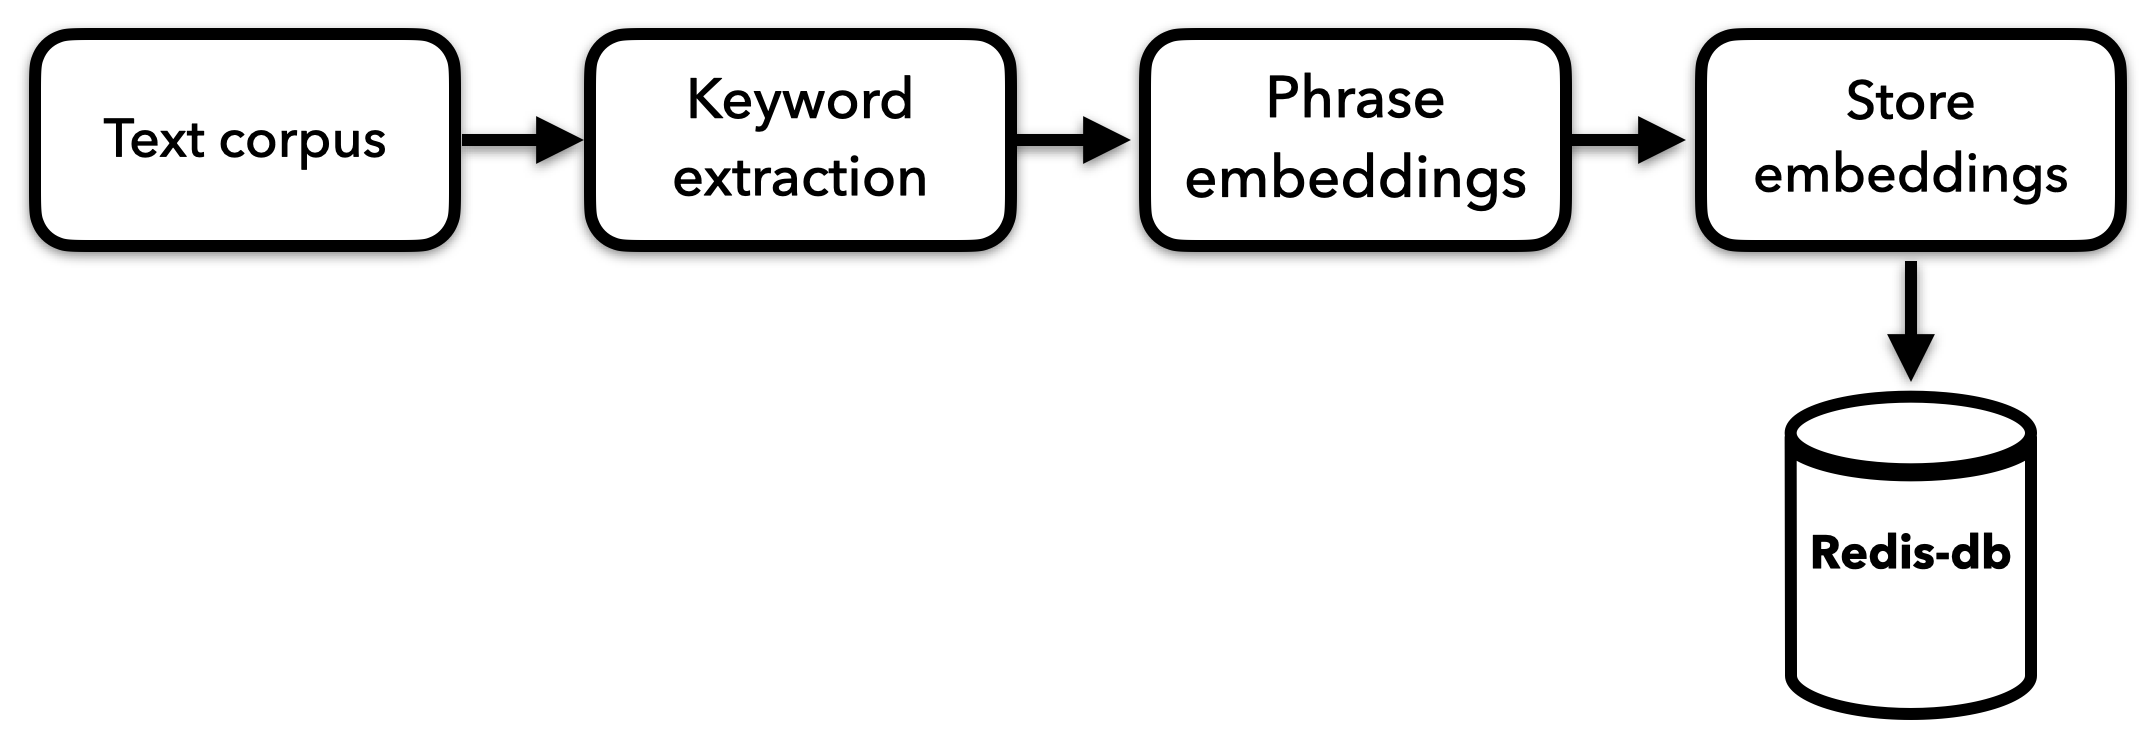
\includegraphics[width=.9\textwidth]{images/thesis_images/redisdb.png}
	\caption[Pjpeline for efficient sub-topics.]{Preprocessing pipeline for efficient sub-topic modeling. \label{fig:redis_db}}
\end{figure}

Manual analysis of sub-topic modeling reveals that the encoding time for a text using a \ac{USE} model is high. This results in users having to wait for a response from the \ac{IR} system. To overcome this, a cache system is developed to store the keyword embeddings obtained from the \ac{USE} model in a \emph{Redis DB}. \prettyref{fig:redis_db} illustrates the pipeline implemented to improve the time required for sub-topic modeling. The performance of sub-topic retrieval using the cache is evaluated against retrieval without using the cache. The mean time taken in seconds for sub-topic retrieval across 28 search queries is considered as the evaluation metric. Let us denote the time taken for retrieving sub-topics for one query $q$ as $t_q$, and the mean time over $N$ queries as $Mt$.


\centerline{$Mt$ = ($\sum\limits_{i=1}^N t_i) /N$}

The approach is considered more efficient when the time taken to retrieve sub-topics is lower. \prettyref{tab:cache_comparision} provides a comparison of the mean time taken in seconds for the two approaches. It is observed that caching keyword embeddings results in sub-topic retrieval that is almost 10 times faster, making it a more efficient approach. Sub-topic retrieval without caching the keywords can take up to one minute, which can negatively impact the usability of this proposed candidate keyword selection approach in real-time.


\begin{center}
	\captionof{table}[Performance comparison of caching.]{Performance comparison of caching keyword embeddings.}\label{tab:cache_comparision}
	\begin{tabularx}{0.77\textwidth}{|Y|Y|}
		\hline
		 Sub-topic retrieval approach &  Mean time taken in seconds ($Mt$) \\
		\hline
	 With caching & \textbf{7.75} \\
		\hline
	 Without caching & 77.41 \\
		\hline
	\end{tabularx}
\end{center}


\section{Clustering Evaluation}

The main objective of this evaluation is to determine the parameters of the sub-topic modeling that create clusters representing the candidate pool in the best and most diverse manner. Since there are no cluster labels available for the queries in the testset, an alternative approach is adopted to assess the quality of the generated clusters.

	
	\subsection{Intrinsic Evaluation} In the case of no labeled data, the clustering output is generally evaluated using an intrinsic evaluation approach. The silhouette score is a metric used for evaluating the clustering performance and is calculated by using the intra-cluster and inter-cluster distances for each sample~\cite{rousseeuw1987silhouettes, shutaywi2021silhouette}. Let us consider the testset $T$ as a set of data points where each data point is denoted as $x_i$.
		
		\centerline{$T$ = $\{x_1, x_2, x_2,\dots\}$}
		
		The testset $T$ is clustered using a clustering algorithm resulting the data points segregated into groups. Let us consider the cluster set $C$ where each cluster is denoted as $c_i$.
		
		\centerline{$C$ = $\{c_1, c_2, c_2,\dots\}$}
		
		The silhouette score $s(x_i)$ for a data point $x_i$ which is an element of cluster $c_k$ is expressed as below.\\
		
		\centerline{$s(x_i)$ = $\frac{b(x_i) - a(x_i)}{max(b(x_i), a(x_i))} $}
		
The value $a(x_i)$ represents the mean distance between the data point $x_i$ and all other data points inside the cluster $c_k$. On the other hand, $b(x_i)$ represents the mean distance between the data point $x_i$ and all other data points in the nearest cluster $c_l$~\cite{shutaywi2021silhouette}. These values, $a(x_i)$ and $b(x_i)$, respectively represent the intra-cluster and inter-cluster distances. The silhouette score $s(x_i)$ is calculated for all the data points in the testset, and the final mean is considered as the silhouette score $S$ of the clustering. The silhouette score ranges from -1 to 1, with a higher score representing better clustering performance.

		
		\begin{figure}[h]
			\centering
			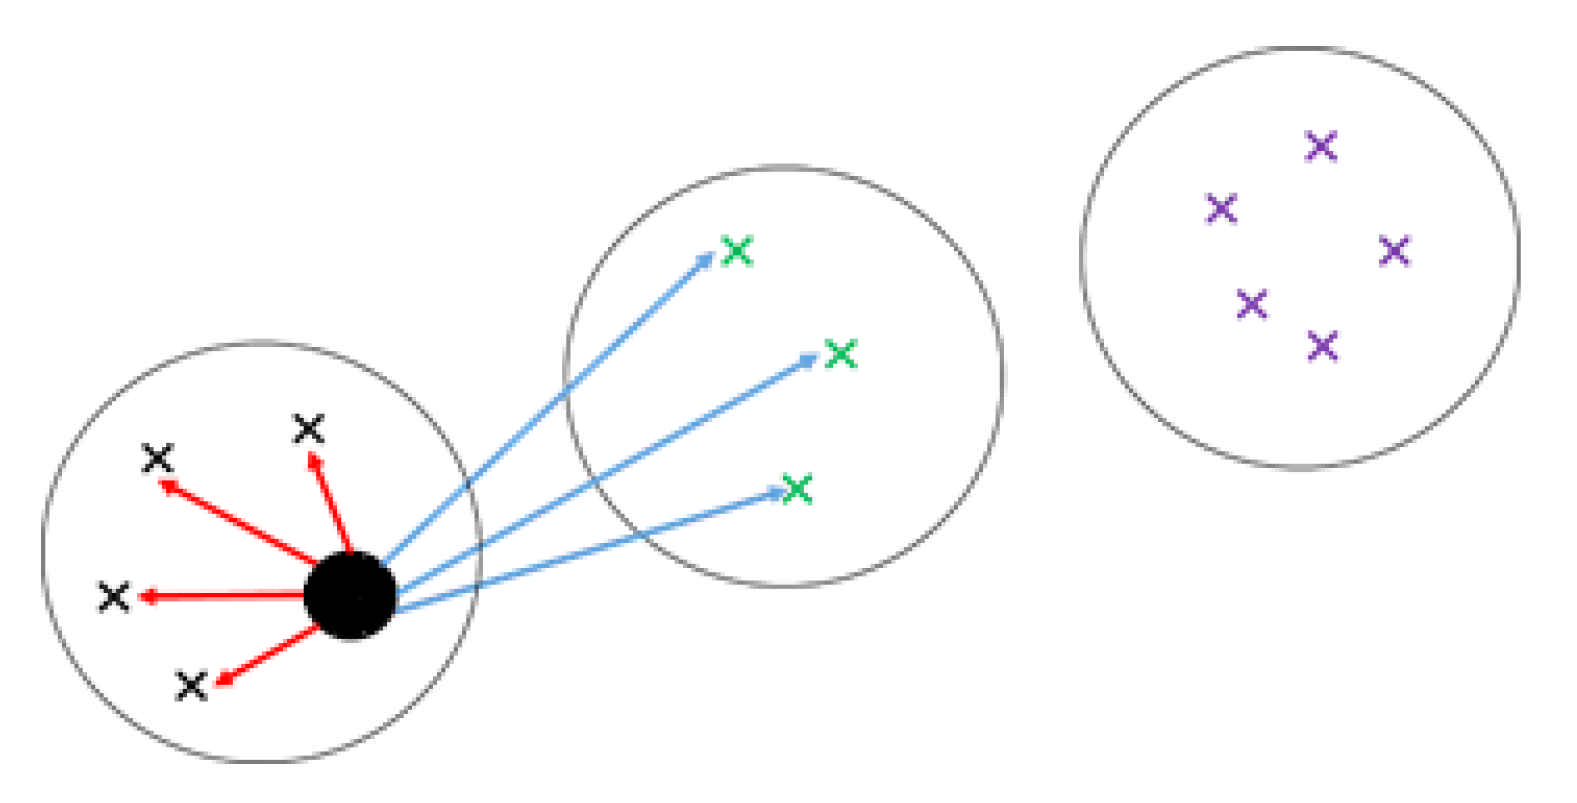
\includegraphics[width=.7\textwidth]{images/papers/silhouette_index.png}
			\caption[Visualization of silhouette score calculation]{Visualization of silhouette score calculation~\cite{shutaywi2021silhouette}.  \label{fig:silhouette_index}}
		\end{figure}
	
The Silhouette score formula is represented for the data point $x_i$ (highlighted in dark) in ~\prettyref{fig:silhouette_index}, where the red lines represent the intra-cluster distances $a(x_i)$ and the blue lines represent the inter-cluster distances to the nearest cluster $b(x_i)$. In the best-case scenario, the value of $a(x_i)$ is very low compared to the value of $b(x_i)$, which results in well-formed clusters. Therefore, the goal of achieving heterogeneity can be measured using the silhouette score.

	
		\subsection{Extrinsic Evaluation} To evaluate the quality of clustering with the help of document labels in the testset, a custom target function $F$ is designed. The target function $F$ tests the quality of clusters against the relevance labels from the dataset. The objective is to determine whether relevant documents are clustered into a similar cluster and the same applies to irrelevant documents. Without any relationship between clustering and relevance labeling, it cannot be assumed that positive and negative documents are automatically clustered together, as they may cover a wide range of keywords in different domains. Therefore, it is more meaningful to evaluate the clustering for negative documents, i.e., irrelevant and wrongly labeled documents. A target function is designed to address the number of negative documents isolated through sub-topic modeling.
		
		
The output of the sub-topic modeling pipeline is distinctive clusters with a unique context, independent of relevance to the user's intention. However, the clusters can be divided into relevant and irrelevant clusters based on the relevance labels in the dataset. Let us consider that $N_1, N_2, N_3, N_4$ represent functions to obtain the number of documents in a single cluster with label IDs $1, 2, 3, 4$ respectively, as shown in \prettyref{tab:label_definitions}, and $C$ represents the cluster set.
		
		\centerline{$C$ = $\{c_1, c_2, c_2,\dots\}$}
		
		Relevant clusters $C_r$ are clusters, that contain at least one document with label-id $1$ or documents with majority of label-id $2$. This can be determined using the below expression.
		
		\centerline{$C_r$ = $\{c_i \in C | (N_1(c_i) > 0) \lor (2 * N_2(c_i) >= (N_3(c_i) + N_4(c_i))) $}
		
		With this expression, relevant clusters are differentiated from others and the focus is only on labels $1$ and $2$. The clusters that do not satisfy the above condition are logically considered irrelevant clusters. 
		
		\centerline{$C_i$ = $\{c_j \in C \setminus C_r\} $}
		
The target function evaluates the clustering by calculating the ratio of irrelevant documents to the documents in the candidate pool $CP_q$ for a given user query $q$. For a total of $N$ queries, the target function maps the score using the equation below. The function $F$ ranges from 0 to 100, where a higher score indicates better separation of negative documents from positive documents, indirectly representing the diversity of clustering results.

		
		\centerline{$F$ = $\sum\limits_{i=1}^N (|C_i|/|CP_i|) * 100 $}
		
		\subsection{Objective Function} Both target functions \emph{silhouette score} and $F$ are used to tune the parameters of the sub-topic modeling pipeline. The silhouette score evaluates the clustering output, and the custom target function $F$ evaluates the distribution of relevant labels. In order to perform automatic parameter selection, an objective function $O$ is proposed, which takes the harmonic mean of \textit{silhouette} and \textit{target function} scores. Since the scores are on different scales, both are normalized to a range [0-1] using \textit{min-max normalization}. Therefore, $O$ ranges from [0-1], and the clustering parameters that generate a higher score are considered as the final sub-topic pipeline parameters. \prettyref{tab:hyper_parameters} shows the hyperparameters that are employed during clustering evaluation.\\
		
		\centerline{$O$ = $ \frac{(2 * S * F)}{(S + F)} $}
		
		\mycomment{An automatic parameter tuning can lead to very small clusters and there is a possibility of documents being marked as noise. Therefore,  A manual evaluation of these two metrics will be considered to finalize the pipeline parameters. }
		
		\subsection{Hyperparameter Selection:}
		
Three main components in the sub-topic modeling pipeline are candidate keyword selection, dimensionality reduction with \ac{UMAP}, and clustering using \ac{HDBSCAN}. Candidate keyword selection has only one parameter ranging from 10 to 100, signifying the percentile selection according to the query similarity. \ac{UMAP} dimensionality reduction has many parameters, but only the output data's reduced dimensions are considered for parameter selection. The other parameters are chosen after some preliminary tests. Two main parameters used in \ac{HDBSCAN} clustering are \textit{minimum cluster size} and \textit{minimum samples}. The minimum cluster size is a crucial parameter that determines the final cluster size of the clusters and is used by \ac{HDBSCAN} to merge clusters until the specified clustering size is achieved. Minimum samples signify the minimum number of neighbors to a core point. The larger the value of this parameter, the resulting clusters are denser, and more data points are labeled as noise points~\cite{hdbscanParameterSelection}. \prettyref{tab:hyper_parameters} shows the parameters used for clustering evaluation.

		
		
		\begin{center}
			\captionof{table}{Parameters used in the pipeline for testing.}\label{tab:hyper_parameters}
			\begin{tabularx}{.9\textwidth}{|Y|Y|}
				\hline
				Hyperparameters & Range  \\
				\hline
				 Candidate keyword selection parameter & [10, 15, 20, 25, 30, 35, 40, 45, 50, 55, 60, 65, 70, 75, 80, 85, 90, 95, 100]  \\
				\hline
				 Reduced dimensions (\ac{UMAP}) & [5, 10]  \\
				\hline
				 Min cluster size (\ac{HDBSCAN}) & [20, 25, 30, 35, 40, 45, 50, 55, 60 ]  \\
				\hline
				 Min samples (\ac{HDBSCAN}) & [1, 3, 5, 7, 10 ] \\
				\hline
			\end{tabularx}
		\end{center}
	  



\section{Survey Evaluation}

The sub-topics are assumed to help the user by retrieving the documents that are related to the query and sub-topics. This can be referred to as the assumption of user satisfaction. Precision analysis can evaluate this assumption when a dataset with two inputs rather than one input is available. Two inputs here denote the original query and an additional sub-topic. As \ac{FKIE} is keenly interested in specific topics of technology and the military, and the user intention is also restricted to the innovation-related theme, a manual evaluation with the help of a survey is chosen.


Two \ac{IR} systems, namely \emph{System A} and \emph{System B}, are designed to represent the documents during retrieval when a query and sub-topic are provided. This survey evaluates the performance of these two \ac{IR} systems. Template queries are used to retrieve and rank the text documents semantically. A template ``Innovation in \textbf{Query} and \textbf{Sub-topic}'' is used in the retrieval. The \emph{Query} and S\emph{ub-topic} are used as placeholders in the template and are dynamically replaced by actual values the user provides. In addition to evaluating the system, the sub-topic modeling output is also tested by taking the user's feedback on the quality of the sub-topics. Below are the two \ac{IR} systems developed and evaluated in the survey.


\begin{enumerate}
	\item 	\textbf{System A} is an \ac{IR} system that retrieves documents from the sub-topic cluster chosen by the user and re-ranks the retrieved documents using template similarity. Cosine similarity is used as the ranking function. \prettyref{fig:systemA} shows the pipeline to extract documents with system A.
	
	
\begin{figure}[h]
	\centering
	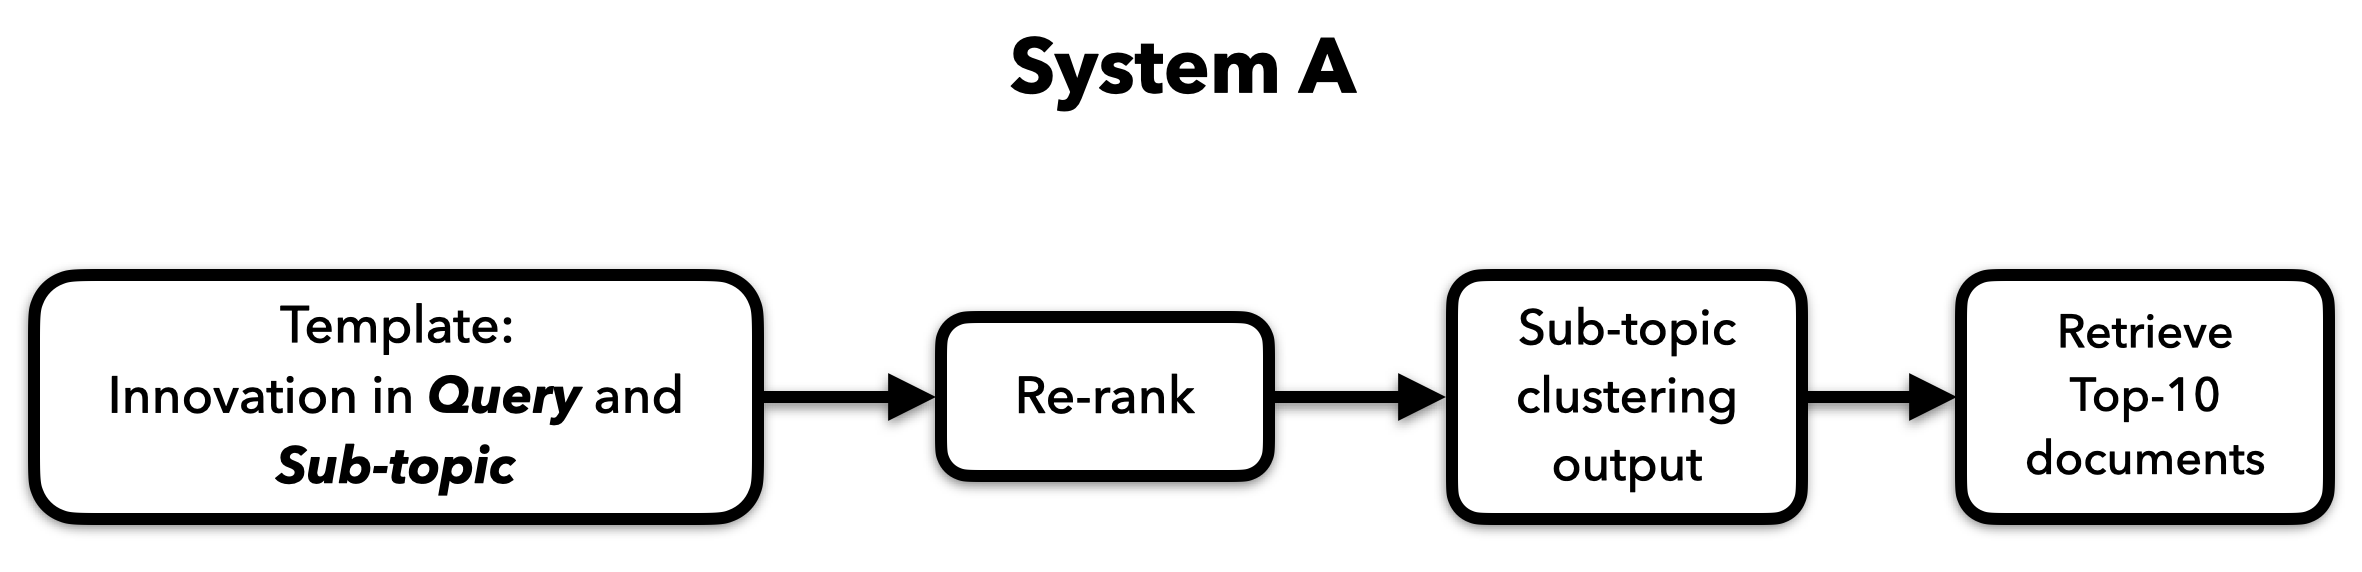
\includegraphics[width=.9\textwidth]{images/thesis_images/systemA.png}
		\caption{Steps to retrieve system A results. \label{fig:systemA}}
\end{figure}
	
	\item 	\textbf{System B} is an \ac{IR} system that retrieves documents semantically using a new search query generated by the template. As the documents are retrieved semantically, there is no need to re-rank the documents again. \prettyref{fig:systemB} shows the pipeline to extract documents with system B.
	
	
	\begin{figure}[h]
		\centering
		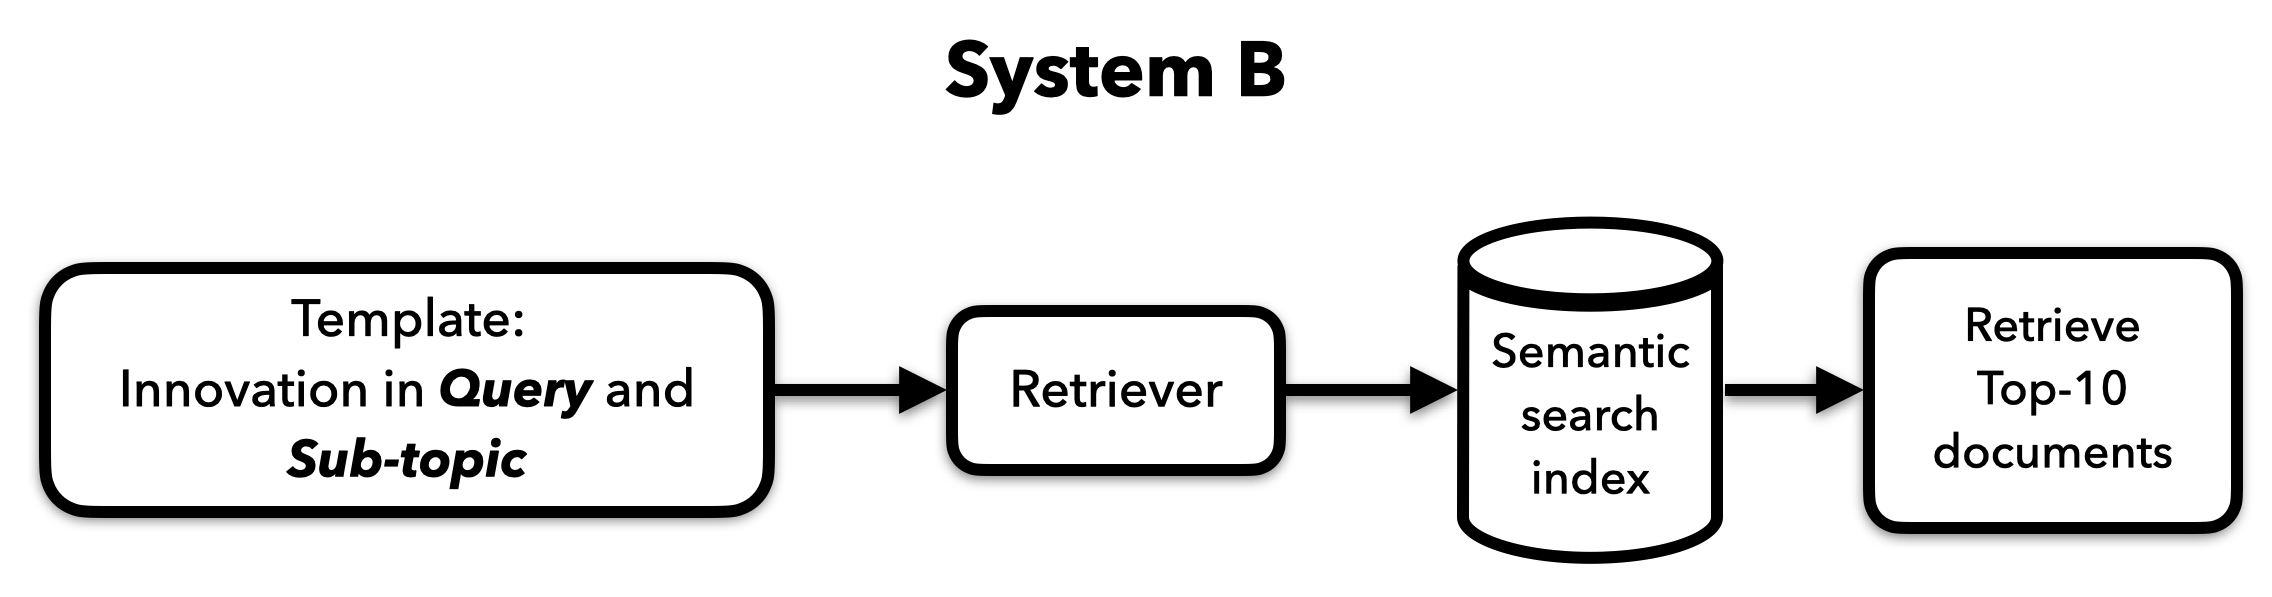
\includegraphics[width=.9\textwidth]{images/thesis_images/systemB.png}
		\caption{Steps to retrieve system B results. \label{fig:systemB}}
	\end{figure}
	
\end{enumerate}

\subsection{Survey questionnaire}

A website is developed to conduct the survey and collect participant data. The feedback collected is stored in an \emph{SQLite DB}. The participants of this survey are employees at \ac{FKIE}. The participants are invited through an email (not chosen by any particular means), and no personal user information is collected during the survey. Only a \ac{UUID} is used to differentiate users when filling out the survey concurrently. The user interface is developed in Python, FastAPI, Bootstrap, \ac{HTML}, and \ac{JS}, and deployed using Docker on the \ac{VM} (detailed definitions are provided in Appendix \ref{appendix:A}). The code developed for the survey questionnaire is shared in a GitHub repository \emph{Survey-thesis}\footnote{\url{https://github.com/praveengadiyaram369/Survey-thesis}}.


\begin{figure}[h]
	\centering
	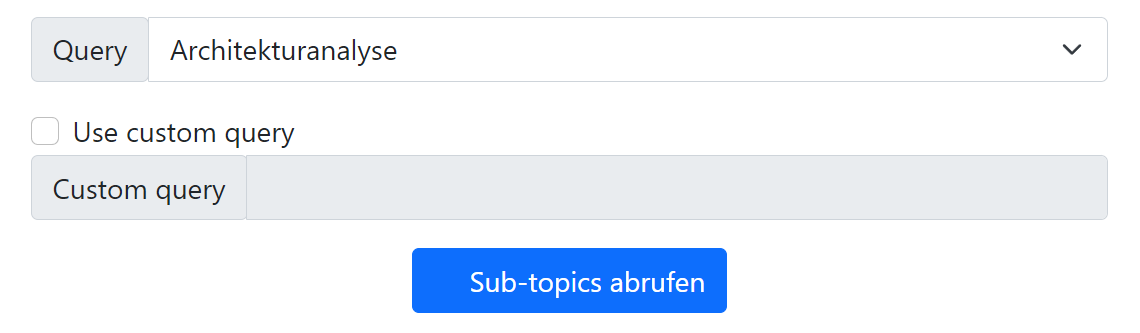
\includegraphics[width=.8\textwidth]{images/survey/query_input.png}
	\caption[Query input from the user.]{Survey UI showing query input either from the dropdown menu or a custom input. \label{fig:survey_question_1}}
\end{figure}

Five questions are developed to evaluate user satisfaction with the retrieved results and sub-topic modeling output. Survey participants are requested to provide a query either by selecting a query from the drop-down list or entering custom text through a text box. ~\prettyref{fig:sub_topic_output} depicts the user interface where participants provide the query. The queries provided in the drop-down list are restricted to a specific keyword list that is of interest for \ac{FKIE}. The keyword list contains queries in both English and German languages, and all participants see the same list. The query keywords list used in the survey is shared in Appendix \ref{appendix:B}.



Subsequently, the sub-topics are retrieved during runtime and displayed to the user as a list. \prettyref{fig:sub_topic_output} shows the extracted sub-topic list for the query \emph{Architekturanalyse}. Participants are now asked to share feedback on the quality of this sub-topic list.


Following the feedback, participants are requested to select a sub-topic and retrieve documents relevant to the query and the sub-topic.  \prettyref{fig:survey_question_2} shows the retrieved \ac{IR} system results for the query \emph{Architekturanalyse} and the sub-topic \emph{Mikroprozessor}. Once again, the participants are asked to share feedback on the system results by rating the systems quantitatively. Lastly, the participants are given an optional question regarding the significance of the whole sub-topic approach. The questionnaire used in the survey is briefly described below.


\begin{enumerate}
	\item ~\textbf{Is the above sub-topic clustering output distinctive and well-labeled?} \\
	
This question aims to evaluate the effectiveness of the approach proposed in the master thesis, i.e., well-formed heterogeneous clusters. Participants are requested to share feedback on the clustering output based on two characteristics, namely the distinctiveness and readability of the sub-topics. \prettyref{fig:sub_topic_output} shares the sub-topic clustering output for the query \emph{Architekturanalyse}. Distinctiveness describes the diversity of sub-topics, and readability depicts the ease of understanding the sub-topic by its name or label. The definitions of the labels are not explicitly provided to the participants as they are self-understanding. Below are the options provided to the survey participants, and only one option must be selected.

	
	\begin{enumerate}
		\item Distinctive and well-labeled
		\item Distinctive and not well-labeled
		\item Not distinctive and well-labeled
		\item Not distinctive and not well-labeled
	\end{enumerate}
	
	
	\begin{figure}[h]
		\centering
		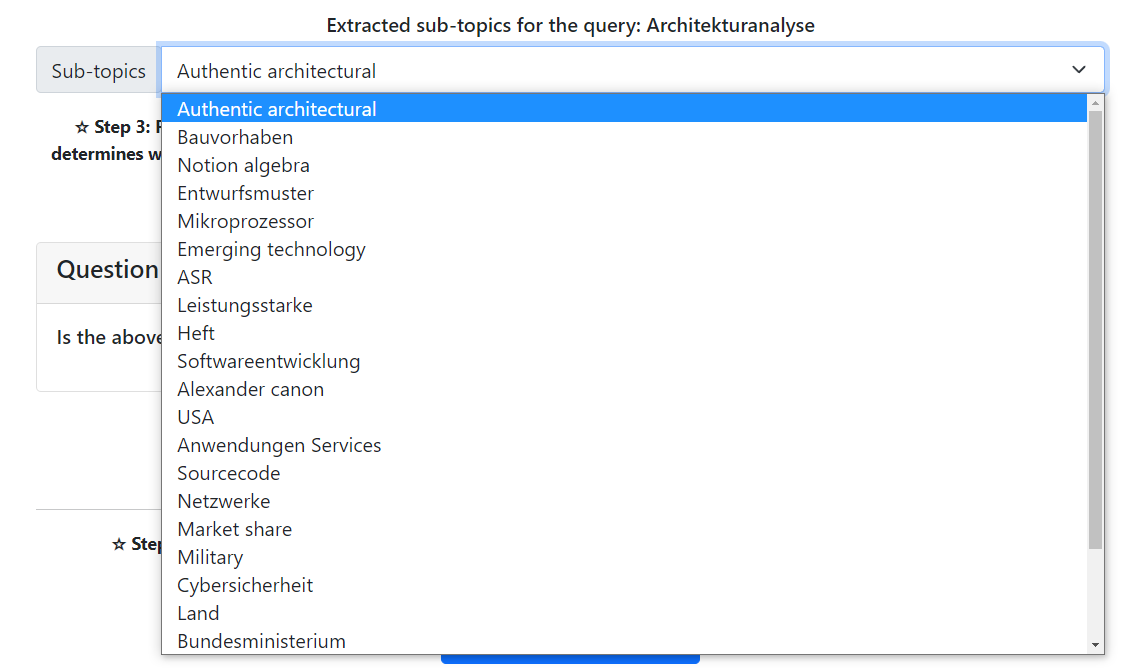
\includegraphics[width=.8\textwidth]{images/survey/sub-topic-output.png}
		\caption[Sub-topic list example.]{Extracted sub-topic list for the given query "Architekturanalyse". \label{fig:sub_topic_output}}
	\end{figure}
	
	
	\item ~\textbf{Which system results better represent the relevant news articles according to the given query and sub-topic?}  \\
	
Relevant news articles are retrieved text documents that have positive document characteristics (mentioned in Section 6.2). Participants are asked to read the retrieved results from \ac{IR} systems A and B and then share the feedback accordingly. \prettyref{fig:survey_question_2} shows the user interface with the system results. Below are the options provided to the survey participants, and only one option must be selected.

	
	\begin{enumerate}
		\item System A
		\item System B
		\item Neither System A nor System B
	\end{enumerate}
	
	\begin{figure}[h]
		\centering
		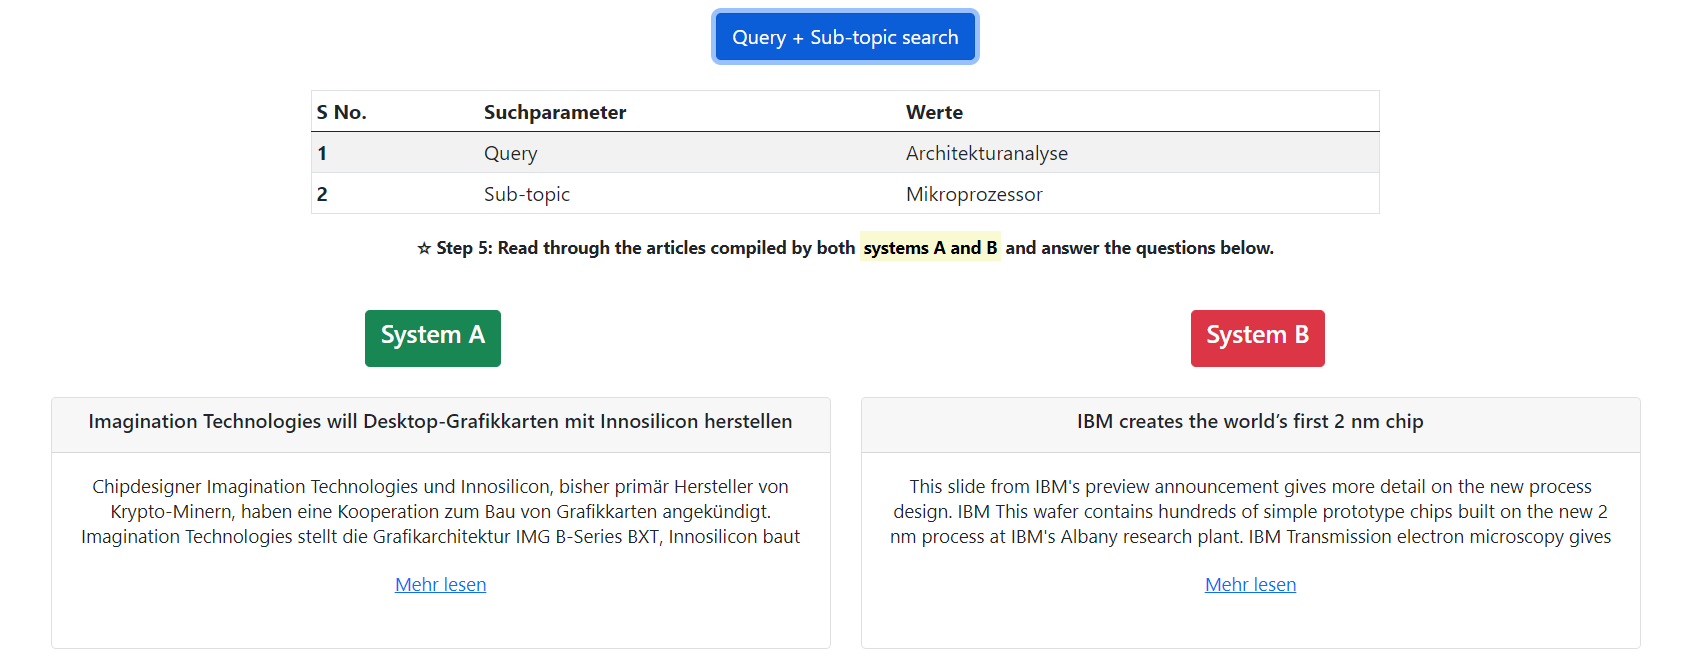
\includegraphics[width=.9\textwidth]{images/survey/sub-topic-search-output.png}
		\caption[Extracted \ac{IR} system results.]{Extracted \ac{IR} system results for a given user query and sub-topic. \label{fig:survey_question_2}}
	\end{figure}
	
	\item ~\textbf{Rate the retrieval system A results for the given query and sub-topic (0-10).} \\
	
Participants are requested to share quantitative feedback by rating the system's results A on a scale of 0 to 10. Ratings can include fractional values up to 1 decimal place. For example, a user can provide a rating of 3.4 but not 4.65. The user ratings directly indicate the user satisfaction corresponding to the retrieved results.

	
	\item ~\textbf{Rate the retrieval system B results for the given query and sub-topic (0-10).} \\
	
	Participants are requested to share a quantitative feedback by rating the system B results between 0 to 10.
	
	\item ~\textbf{Were the sub-topics helpful for you to find the relevant documents?} \\
	
This question aims to evaluate the usefulness of sub-topic modeling in \ac{IR}. It answers the practicality of using the proposed methodology in this master's thesis in a real environment to find innovation-related documents. Participants are requested to provide a boolean response of either "Yes" or "No" corresponding to whether it fulfills their expectations.

	
	\begin{enumerate}
		\item Yes
		\item No
	\end{enumerate}
	
\end{enumerate}

\section{Precision evaluation}

Assuming that the cluster labels could be more helpful to the user, the next evaluation technique shows that the clustering output does not deteriorate the performance of the retrieval results. The clustering output is difficult to examine with the baseline \ac{IR} systems because the order of documents needs to be included, and the performance metrics related to false positives need to be addressed. For this purpose, the sub-topic creation is extended with sub-topic ranking and document ranking. These two rankings help the existing pipeline to create a sequential order of documents and facilitate the evaluation of precision against the baselines. Therefore, this evaluation approach proposes eight different retrieval systems and evaluates the ranked results.


\begin{center}
	\captionof{table}{Proposed \ac{IR} systems for evaluation.}\label{tab:ir_systems}
	\begin{tabularx}{0.8\textwidth}{|c|c|Y|}
		\hline
		 IR system name & Sub-topic ranking & Document ranking \\
		\hline
		 IR0 & NA & Uniform distribution \\
		\hline
		 IR1 & NA & Query similarity \\
		\hline
		 IR2 & Query similarity & Query similarity \\
		\hline
		 IR3 & Template similarity & Template similarity \\
		\hline
		 IR4 & Document cardinality & Query similarity \\
		\hline
		 IR5 & (IR4, IR2) & Query similarity \\
		\hline
		 IR6 & (IR4, IR2, IR3) & Query similarity \\
		\hline
		 IR7 & Random combinations & Query similarity \\
		\hline
	\end{tabularx}
\end{center}

The first system, \emph{IR0}, is an arbitrary system where the positive documents are uniformly distributed in the ranking order. \emph{IR1} system is a simple query re-ranking of results based on cosine similarity between the query and documents. The systems \emph{IR2, IR3, IR4} are the results of sub-topic pipeline clustering, where the clusters are first ranked, and later the documents are re-ranked with certain criteria. These three systems simulate the user reading the results linearly or in a sequence. In \emph{IR2}, the sub-topic clusters are ranked by the cosine similarity between the query and the centroid vector of the cluster, and similarly for document ranking.


The system \emph{IR3} uses a template similarity criterion, where the similarity is calculated between a template and centroid vector rather than the query. For example, the template string used in the master thesis is \emph{Innovation and Technology}. Similarly, \emph{IR4} clusters are ranked using the number of documents in the cluster. The last system, \emph{IR7}, is an unreal system just like \emph{IR0}, but multiple combinations of random rankings of clusters are considered to simulate the random selection of a sub-topic by the user and reading the documents in different sub-topics.


\subsection{Combinational IR systems}

The systems \emph{IR5} and \emph{IR6} are produced by combining sub-topic rankings of other \ac{IR} systems. The sub-topics are combined in such a way that the top-ranking sub-topics are clustered together. This approach adopts the benefits of two ranking criteria into a ranking. As a part of the exploratory analysis, the potential of sub-topic ranking is analyzed with these combinations. Algorithm \prettyref{algo:combined_ir} details the steps to generate a unique combined ranking output in the case of two individual rankings.


	\begin{algorithm}[H]
	\SetKwInput{KwInput}{Input}                % Set the Input
	\SetKwInput{KwOutput}{Output}              % set the Output
	\DontPrintSemicolon
	
	\KwInput{ranking\_lists - list $[ranking\_lists\_i]$, $i=1, 2, \cdots, n$, where each element is an individual ranking list }
	\KwOutput{combined\_ranking\_list - list $[combined\_ranking\_list\_i]$, $i=1, 2, \cdots, n$, where each element is a string }
	% \KwData{Testing set $x$}
	
	% Set Function Names
	\SetKwFunction{FRemovdup}{Combine\_individual\_ranking}
	
	% Write Function with word ``Function''
	\SetKwProg{Fn}{Function}{:}{}
	\Fn{\FRemovdup{$ranking\_list$}}{
			
		\;
		combined\_ranking\_list = []\;
		ranking\_list\_1 = ranking\_list[0]\;
		ranking\_list\_2 = ranking\_list[1]\;
		
		ranking\_list\_len = len(ranking\_list\_1)\;
		
		\;
		
		\For{$i\gets1$ \KwTo $ranking\_list\_len$}{
			
			\tcp{rank\_1 and rank\_2 signifies the ranking id of the sub-topics}
			
			rank\_1 = ranking\_list\_1 [$i$]\;
			rank\_2 = ranking\_list\_2 [$i$]\;
			\;

			\tcp{Append only if the rank id is not added to the combined ranking list}
			
			\If{rank\_1 not in combined\_ranking\_list}
			{
				combined\_ranking\_list.append(rank\_1))\;
			}
			\;
			
			
		   \If{rank\_2 not in combined\_ranking\_list}
			{
				combined\_ranking\_list.append(rank\_2))\;
			}
			\;
			
		}
		\KwRet combined\_ranking\_list\;
	}
	
	\caption{Generate combinational IR system.} \label{algo:combined_ir}
\end{algorithm}
 
The idea of ranking combinations is influenced by ensemble techniques in \ac{ML}. Ensemble methods improve performance and create robust models by combining the strength of multiple weak-performing models ~\cite{bi2019machine}. This technique eliminates the individual model bias and consolidates the unique benefits of individual models. The output of combined \ac{IR} systems presents the opportunity to test a unique ranking of sub-topics. This unique ranking of sub-topics creates a unique sequential order of documents. Following Algorithm \prettyref{algo:combined_ir}, an example of the combined ranking output is presented in \prettyref{tab:ir5_result}. 
\\

 
 
 \begin{center}
 	\captionof{table}{An example of a combined IR5 system result. }\label{tab:ir5_result}
 	\begin{tabularx}{0.8\textwidth}{|c|c|Y|}
 		\hline

 			IR system & Sub-topic ranking type & Ranking list of sub-topics \\
 		\hline
 		IR4 & Document cardinality  & [4, 3, 1, 2, 0] \\
 		\hline
 		IR2 & Query cardinality  & [1, 3, 0, 4, 2] \\
 		\hline
 		IR5 & (IR4, IR2) & [4, 1, 3, 0, 2] \\
 		\hline
 	\end{tabularx}
 \end{center}
 

\subsection{IR systems evaluation}

Mehlitz et al.~\cite{mehlitz2007new} have introduced a new evaluation measure for \ac{IR} systems named the \emph{Expectation score}. The expectation score ($E$) is similar to precision ($P$) but does not consider false positives. $E_k$ represents the number of positive documents at index $k$, whereas $P_k$ represents the ratio of positive documents at index $k$ to $k$. Similarly, the \ac{ME} is proposed to analyze the mean number of positive documents for $N$ queries. This metric is especially useful for comparing \ac{IR} systems that retrieve the most relevant documents at a given index $k$.



\centerline{$ME@k$ = ($\sum\limits_{i=1}^N E_i@k) /N$}

Furthermore, Mean Average Precision (MAP)~\cite{cormack2006statistical} is used to evaluate the ranking performance. MAP is calculated through the Average Precision (AP) metric, which is an average of precision scores only at the positive document indices. Let us consider that $G$ is a set of all positive document indices with size $g$. The average precision and mean average precision are formulated as below. MAP alone is sufficient to compare different \ac{IR} systems, and the system with the highest MAP value is considered the best \ac{IR} system.


\centerline{$AP$ = ($\sum\limits_{i=1}^G P_i) /g$}

\centerline{$MAP$ = ($\sum\limits_{i=1}^N AP_i) /N$}

\subsection{Literature Comparison}

Sub-topic retrieval has two crucial components, namely \emph{sub-topic creation} and \emph{document retrieval}. Sub-topic creation generates representations from large news articles for a given search query. Document retrieval deals with the extraction of ranked news articles for a given search query and sub-topic. In the end, the output of sub-topic retrieval is nothing but a ranked list of news articles. Therefore, the output of the proposed approach in this master thesis is compared with the literature work shared by Nogueira and Cho~\cite{nogueira2019passage}. This retrieval approach from the literature is known as \emph{Passage Re-ranking with \ac{BERT}}, and it uses contextual representations from \ac{BERT} language models to retrieve and re-rank the text documents.



Passage Re-ranking approach uses a \emph{multi-stage ranking} architecture and is presented in Section 4.2 of Chapter 4. The compared literature has similar goals to the proposed approach, such as unsupervised, multi-lingual, contextual representations, and two-stage retrieval (for high recall). The literature uses \emph{Retriever} and \emph{Re-ranker} components, which retrieve candidate documents based on certain criteria and rank the retrieved documents, respectively. This approach was initially proposed for question-answering tasks. To generate candidate documents for a search query, three different techniques are employed, namely \emph{BM-25}, \emph{Bi-encoder retrieval}, and \emph{Candidate pool extraction}.


\begin{figure}[h]
	\centering
	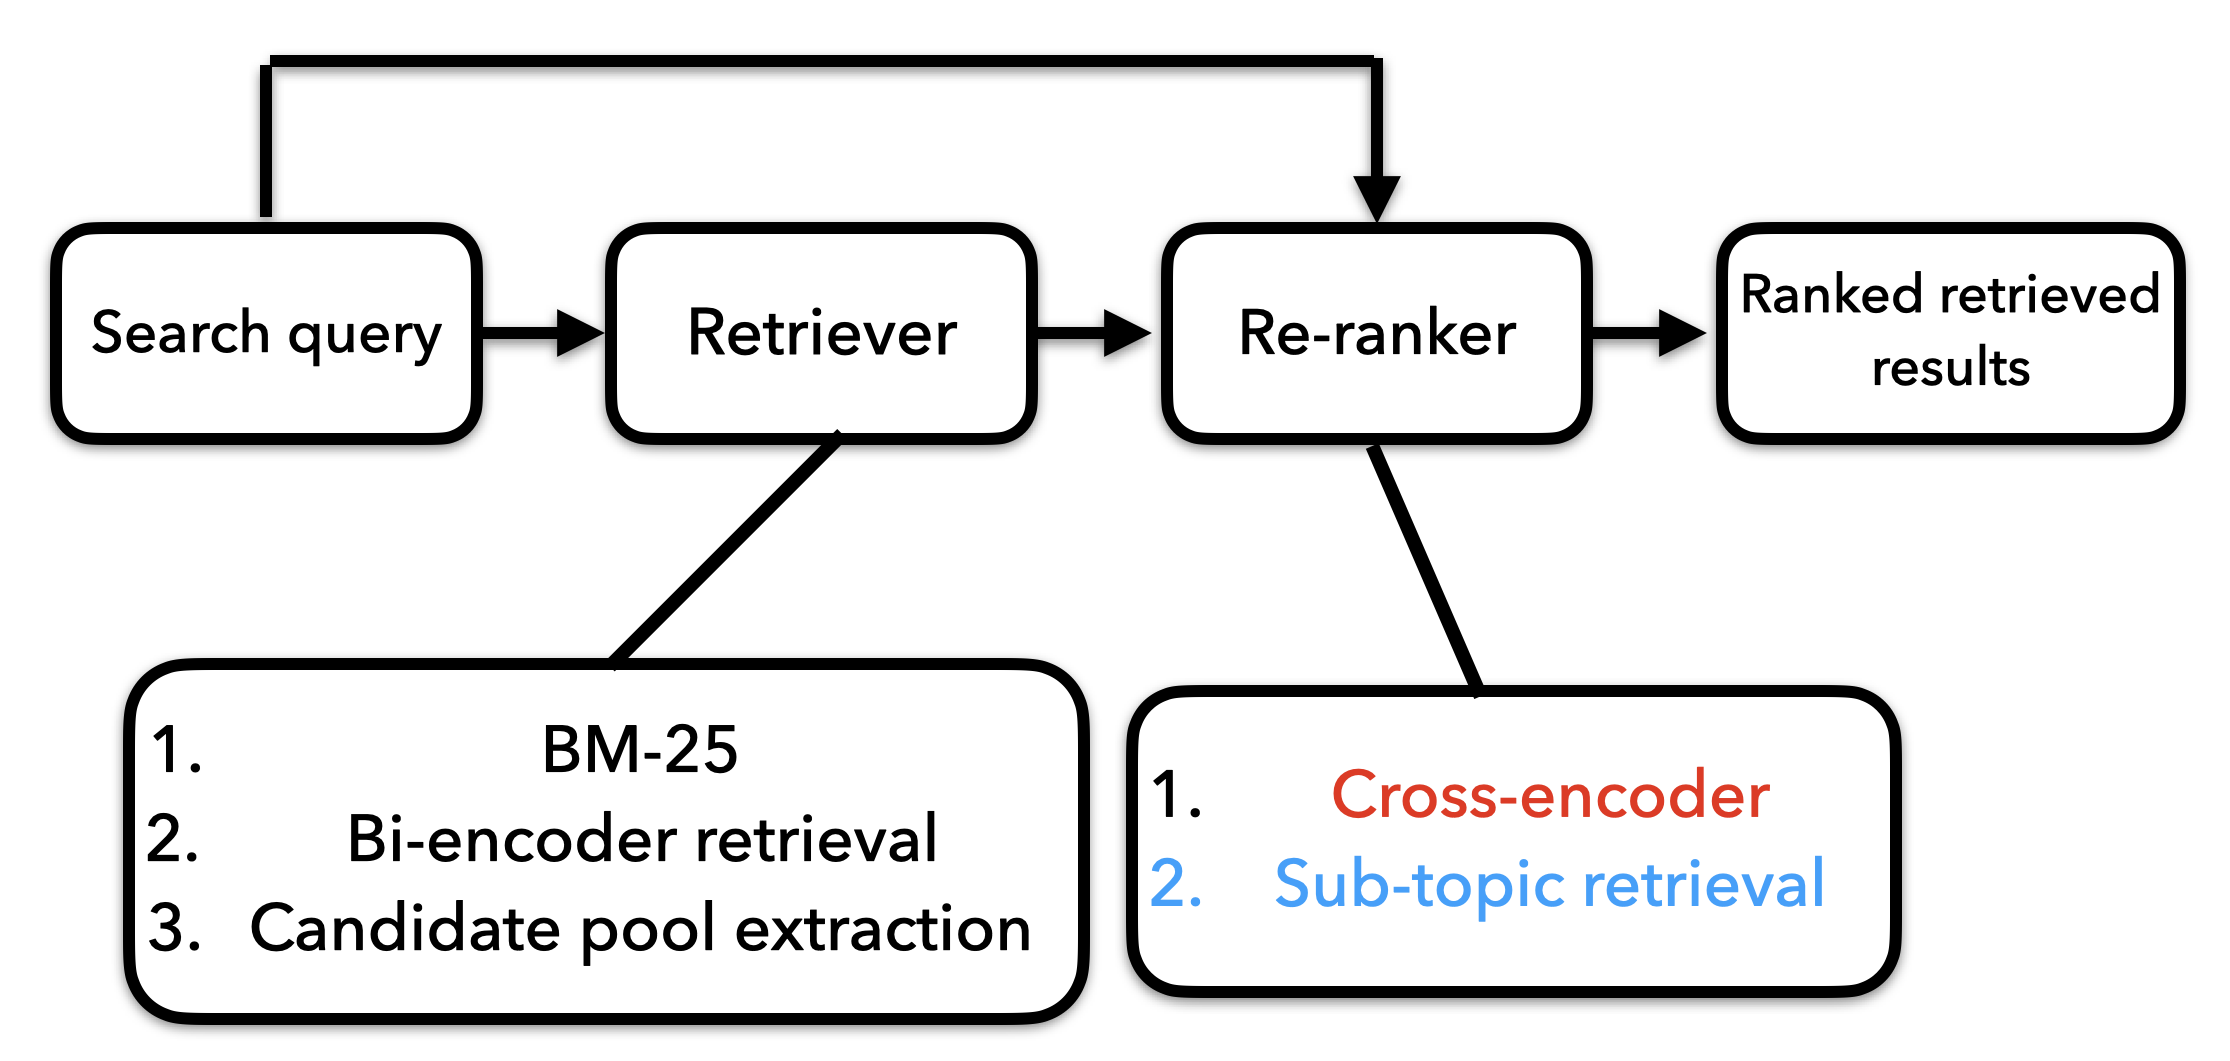
\includegraphics[width=.9\textwidth]{images/thesis_images/literature_review.png}
	\caption{Multi-stage ranking architecture. \label{fig:literature_review}}
\end{figure}

\begin{description}
	\item[BM-25]  \hfill \\ BM-25 is a probabilistic relevance algorithm which uses lexical matching approach to retrieve documents similar to the search query~\cite{amati_bm25_2009}.
	
	\item[Bi-encoder retrieval]  \hfill \\ Bi-encoders are neural network models that encode the query and documents into dense vector representations. The encoded vector representations of the query and documents are then used to calculate the relevance similarity. The documents with higher query similarity are considered as retrieval output. A BERT-based multi-lingual bi-encoder model\footnote{\url{https://huggingface.co/LLukas22/all-MiniLM-L12-v2-embedding-all}} is used in this thesis to facilitate the extraction of candidate documents. The retrieved candidate documents using bi-encoder models are also referred to as the \emph{semantic pool}.
	
	
	\item[Candidate pool extraction]  \hfill \\ Candidate pool extraction is an efficient retrieval method proposed in this master thesis to generate candidate documents for re-ranking. This approach considers both lexical and semantic matching approaches. More details about this approach are shared in Section 5.1 of Chapter 5.
	
\end{description}

The candidate document extraction with BM-25 and bi-encoder is implemented with the help of the script provided by sentence-transformers\footnote{\url{https://github.com/UKPLab/sentence-transformers/blob/master/examples/applications/retrieve_rerank/retrieve_rerank_simple_wikipedia.ipynb}}. Once the candidate news articles are extracted for a search query, the re-ranker ranks them based on query retrieval similarity. The ranking performance of two re-ranking approaches is evaluated using \ac{MAP}. The two approaches are namely \emph{Cross-encoder ranking} and \emph{Sub-topic retrieval}.



\begin{description}
	\item[Cross-encoder ranking]  \hfill \\ Cross-encoders are neural network models that encode the query and documents together and generate the relevance score between -1 and 1. The documents with higher query relevance similarity are considered as retrieval output. A BERT-based multilingual cross-encoder\footnote{\url{https://huggingface.co/amberoad/bert-multilingual-passage-reranking-msmarco}} model is used in this thesis to rank candidate documents generated from retrieval. The ranked results from the cross-encoder are compared to the proposed approach in the master thesis.
	
	
	\item[Sub-topic retrieval]  \hfill \\ The sub-topic retrieval output contains two ranking techniques to generate the final ranking of news articles. The first ranking technique is sub-topic cluster ranking, followed by document ranking. Eight different \ac{IR} systems with unique sub-topic and document rankings are proposed in Section 6.6, as shown in \prettyref{tab:ir_systems}. The system that performs the best is compared with the ranking output of the cross-encoder.
	
	
\end{description}


\section{Evaluation summarization}

The \prettyref{tab:evaluation_rq} shares the evaluation techniques chosen in this master thesis and the respective research questions answered.

\begin{center}
	\captionof{table}{Proposed evaluation techniques. }\label{tab:evaluation_rq}
	\begin{tabularx}{0.9\textwidth}{|c|Y|Y|}
		\hline
 		S No. & Evaluation type & Research questions addressed \\
		\hline
		1 & Clustering analysis  & \textbf{RQ1} \\
		\hline
		2 & Survey questionnaire  & \textbf{RQ1, RQ2} \\
		\hline
		3 & Precision analysis and literature comparison & \textbf{RQ3} \\
		\hline
	\end{tabularx}
\end{center}






        % !TEX root = ../thesis.tex

\chapter{Experiment Results}

In this chapter, the evaluation results are shared, and the three research questions are answered. Similar to the experiment setup, the experiment results are divided into three sections, namely "Clustering Results Evaluation", "Survey Results Evaluation", and "Precision Analysis Results". A few experiment results are separately shared according to different sizes of the candidate document pool. Moreover, the ineffectiveness of certain experiment results is assessed with critical reasoning. The section "Precision Analysis Results" shares the outcome of the exploratory analysis and literature comparison.

\section{Clustering Results Evaluation}

As the testset contains 17 user queries and the clustering analysis is performed on each query, and the output is analyzed based on the mean values of the clustering output. Two candidate pools are generated for each query with sizes 30 and 100, respectively. The small candidate pool (CP-30), and the large candidate pool (CP-100), represent the retrieved results of the original query from both syntactic and semantic matching. CP-30 contains a maximum of 30 labeled documents. CP-100 contains around 100 documents, and only a few documents present in the testset are labeled. Therefore, more than half of the CP-100 documents are unlabeled. The unlabeled documents are removed from the clustering output during the analysis, and only the labeled documents are used for evaluation. This assumes that having more documents in CP-100 helps to provide better clusters compared to CP-30. Furthermore, it is expected to extract better sub-topics from the larger collection in order to gain deeper insights into the data.

\subsection{Clustering Output Analysis}

The sub-topic modeling pipeline is tested on all the hyperparameters of clustering mentioned in Section 6.4.3. Ideally, there should be 1,710 cases to test the clustering output for small and large candidate pools. However, a few test cases have produced very low clustering (only one cluster) and are not considered in the parameter selection. Ultimately, 1,588 and 1,009 possible hyperparameter combinations are evaluated for large and small candidate pools, respectively. The clustering output consisting of the evaluation metrics, is expressed as the mean over all 17 queries. Furthermore, the analysis is shared separately for the small and large candidate pools. In the analysis below, "silhouette score" denotes the intrinsic evaluation metric, and "targeted negative document ratio" signifies the extrinsic evaluation metric that denotes the quality of separation between relevant and irrelevant clusters.

\ac{HDBSCAN} clustering does not require any parameter to specify the number of clusters created from the data. On the other hand,  hyperparameters need to be well chosen to generate better clusters. Before evaluating the parameters that significantly affect the clustering output, the relation between the evaluation metrics and the number of clusters is analyzed.  \prettyref{fig:silhouette_score_vs_cc} shows the relationship between the silhouette score and the number of clusters. The data is generated when all the hyperparameter possibilities of the clustering pipeline are tested over the testset queries.

\begin{figure}[h]
	\centering
	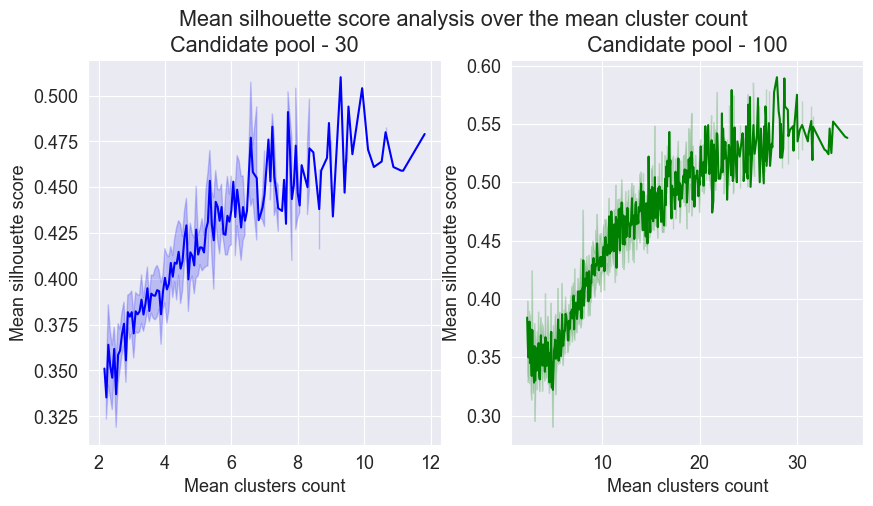
\includegraphics[width=.99\textwidth]{images/subplots/sil_score_ccnt_subplot.png}
	\caption{Silhouette score analysis over clusters count. \label{fig:silhouette_score_vs_cc}}
\end{figure}

The objective of this analysis is to observe whether the number of clusters has an impact on the silhouette score globally. This means that the overall effect of cluster counts is not specific to a particular query or a hyperparameter set. It is clear from \prettyref{fig:silhouette_score_vs_cc} that a relatively high number of clusters generates higher silhouette scores, implying better cluster quality. However, high number of clusters in both small and large candidate pools show lower silhouette scores than the highest value. This signifies that a high number of clusters can result in many clusters with very few data points, reducing the quality of clustering as the silhouette score is based on intra- and inter-cluster distances. The best clustering can be achieved when the intra-cluster distance is minimized and the inter-cluster distances are maximized. Therefore, a small number of clusters leads to overlapping clusters (very close) and is not a good choice for clustering parameter selection.

\begin{figure}[h]
	\centering
	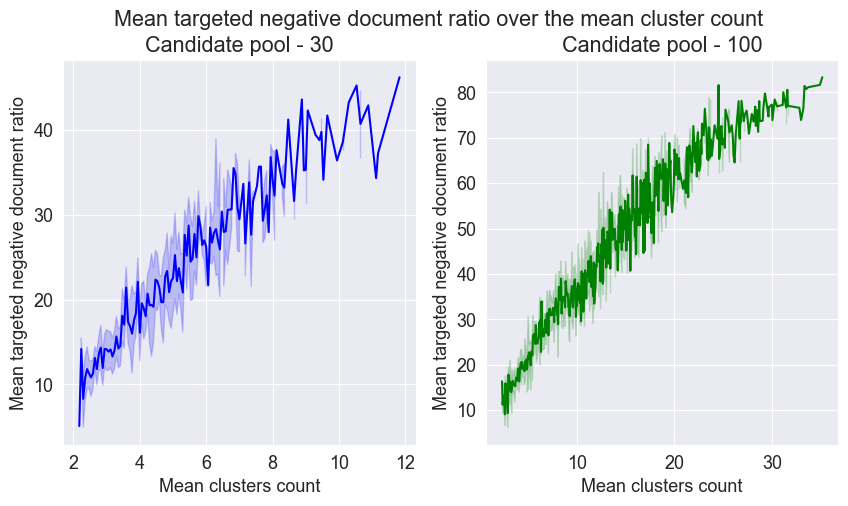
\includegraphics[width=.99\textwidth]{images/subplots/targetfn_score_ccnt_subplot.png}
	\caption[Targeted negative document ratio analysis.]{Targeted negative document ratio analysis over cluster count.  \label{fig:target_function_vs_cc}}
\end{figure}


It is assumed that the heterogeneity or diversity of clusters can be derived from the cluster quality, and to have a wide variety of clusters, the parameters that create a high number of clusters must be selected. One major drawback of this analysis is the combination of all the clustering outputs for all 17 queries in the testset. Some queries generate a low number of clusters, while others generate a high number of clusters. Combining all queries into one analysis may lead to misleading results in certain scenarios. However, since the focus is on observing the overall impact of the number of clusters, the analysis can still be considered for parameter selection without any issues.

\mycomment{
	~\prettyref{tab:correlation_data} shows the Pearson correlation
	over all the hyperparameters tested, and there is a positive correlation between the cluster
	count and evaluation metrics chosen.
	
	\begin{center}
		\captionof{table}{Pearson correlation between the clustering observations.}\label{tab:correlation_data}
		\begin{tabularx}{.99\textwidth}{|Y|c|c|}
			\hline
			Parameter & CP-30 & CP-100 \\
			\hline
			Mean silhouette score and mean clusters count & 0.71 & 0.89 \\
			\hline
			Mean targeted negative document ratio and mean clusters count & 0.76 & 0.94 \\
			\hline
		\end{tabularx}
\end{center}}

 
\prettyref{fig:target_function_vs_cc} shows the relationship between the targeted negative document score and the number of clusters. Similar to the silhouette score, a higher cluster count positively correlates with the targeted document ratio. The design of this evaluation metric slightly favors clustering outputs with a high cluster count, as it creates many clusters with a low number of data points and results in greater separation between clusters. Consequently, fewer clusters indicate poorer cluster quality due to inadequate separation between the documents. Therefore, this metric needs to be relatively higher in order to create a diverse set of clusters with good separation. The large candidate pool has a better silhouette score and targeted negative document ratio compared to the small candidate pool. Since labels for all documents in the large candidate pool are unknown, the actual scores could be even higher than those presented.

\subsection{Candidate Keyword Selection Analysis}
This section explores the impact of the Candidate keyword selection ($cks$) parameter on the clustering output, specifically regarding keyword selection. This analysis is crucial for finalizing the parameter selection. The $cks$ parameter ranges from 10 to 100, with values incrementing by 5, signifying the percentile selection based on query similarity. 

The keywords selected using the $cks$ parameter are further clustered using \ac{HDBSCAN}. One of the main objectives of this master thesis is to test the effectiveness of clustering with keyword selection compared to no selection. The data used in this analysis is generated from clustering results for all possible parameter combinations in the hyperparameter set over the testset queries. The x-axis represents the candidate keyword selection, and the y-axis represents the mean of the respective evaluation metrics.


\begin{figure}[h]
	\centering
	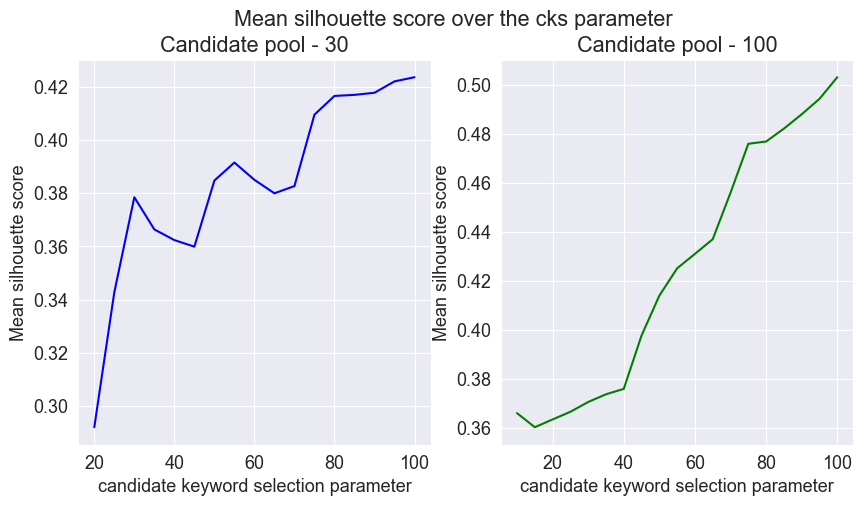
\includegraphics[width=.99\textwidth]{images/subplots/csk_sil_score_subplot.png}
	\caption[Silhouette score analysis over cks parameter.]{Silhouette score analysis over candidate keyword selection parameter. \label{fig:silhouette_score_vs_csk}}
\end{figure}  

 \prettyref{fig:silhouette_score_vs_csk} presents the relationship between the mean silhouette score and the $cks$ parameter. Results from the large candidate pool clearly show that a higher $cks$ parameter generates a better mean silhouette score. This signifies that selecting more candidate keywords is better, and the best clustering outcome is achieved with no keywords are selected ($cks$ = 100). Small candidate pool results partially agree with this outcome, as the highest silhouette score is achieved when no keywords are selected. However, it is observed that the mean silhouette score decreases at around a percentile selection of 30 and 55. This denotes a change in the structure of the clustering output when specific keywords are selected. However, no downtrend in the data implies that keyword selection does not generate better clusters, and only an overall upward trend is observed.

\begin{figure}[h]
	\centering
	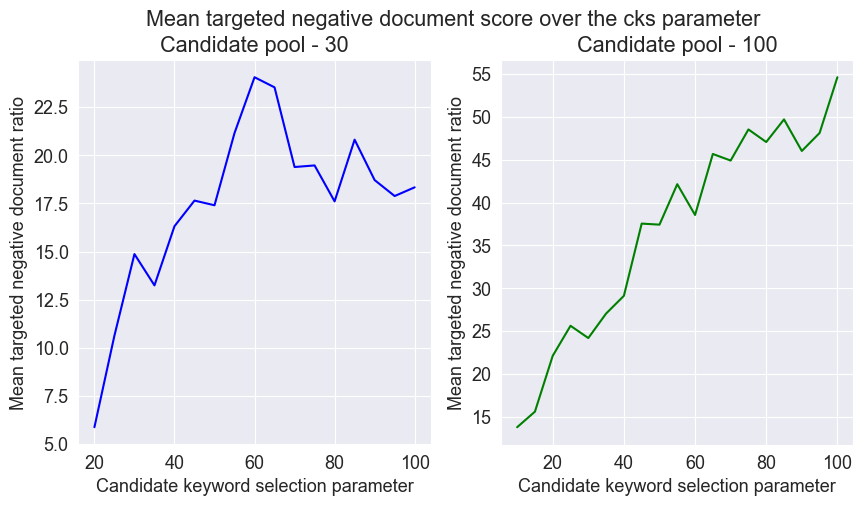
\includegraphics[width=.99\textwidth]{images/subplots/csk_tfn_score_subplot.png}
	\caption[Targeted negative document ratio over cks parameter.]{Targeted negative document ratio over candidate keyword selection parameter.  \label{fig:target_function_vs_csk}}
\end{figure}

\prettyref{fig:target_function_vs_csk} presents the relationship between the mean targeted negative document ratio and the $cks$ parameter. This metric indicates the separation of clusters based on their similarities. The results from the small candidate pool show the highest separation of negative documents at $cks$ = 60 and a downward trend for values of $cks$ higher than 60. This suggests that keyword selection has a positive impact on clustering, achieving better cluster separation. In contrast, the results from the large candidate pool yield different outcomes. There is a clear upward trend, implying that no keyword selection (i.e., $cks$ = 100) has resulted in better separation of clusters. However, the results from the large candidate pool do not truly represent the nature of this evaluation metric, as it ignores the unlabeled documents after clustering. Considering the labels of all 100 documents may lead to different results.

\begin{center}
	\captionof{table}[Mean of evaluation metrics for CP-30.]{Mean of evaluation metrics over the cks parameter for the small candidate pool (30).}\label{tab:top_5_smallcdd}
	\begin{tabularx}{.8\textwidth}{|Y|Y|Y|Y|}
		\hline
		Objective function score &  Mean silhouette score &  Mean targeted negative document ratio &  Cks parameter \\
		\hline
		
		  \textbf{0.48}  &            0.42 &                         20.81 &      85   \\ \hline
		0.46 &            0.41 &                         19.48 &           75 \\ \hline
		0.45 &            0.39 &                         24.06 &           60 \\ \hline
		0.45 &            0.42 &                         18.34 &           100 \\ \hline
		0.45 &            0.42 &                         17.89 &           95 \\ \hline
		
	\end{tabularx}
	
\end{center}

\begin{figure}[h]
	\centering
	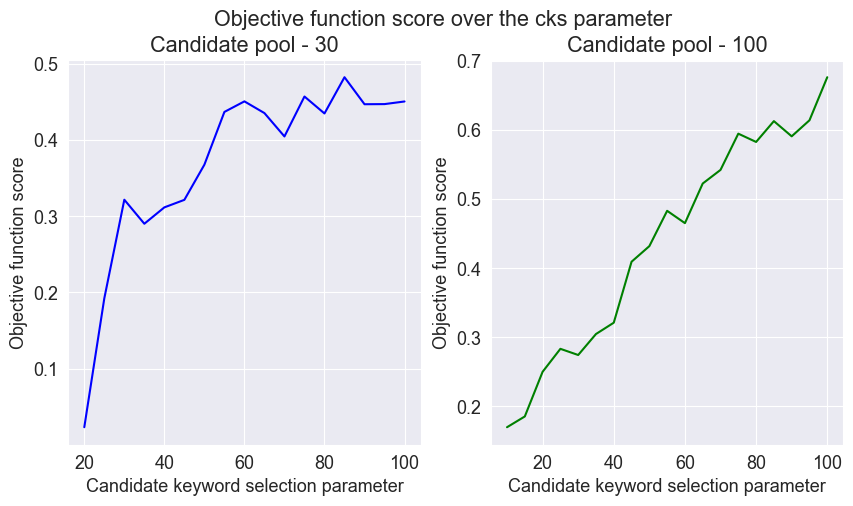
\includegraphics[width=.99\textwidth]{images/subplots/harmonic_score_cks_subplot.png}
	\caption[Objective function score analysis over cks parameter.]{Objective function score analysis over candidate keyword selection parameter. \label{fig:objective_function_vs_csk}}
\end{figure}

The analysis results from intrinsic and extrinsic measures have shown different patterns for the small candidate pool and similar patterns for the large candidate pool. Combining these two measures, a final objective function score, which is the harmonic mean of the normalized intrinsic and extrinsic measures, is calculated. \prettyref{fig:objective_function_vs_csk} presents the relationship between the objective function score and the $cks$ parameter. For the small candidate pool, the highest objective function score is achieved at a keywords selection of 85. This indicates that selecting keywords below the 85th percentile similarity generates better clustering.

However, it is important to note that the top 15 percentile keywords may only consist of around 3 to 4 keywords or even fewer. Therefore, the improvement in clustering between the $cks$ values of 85 and 100 is minimal. Additionally, the keyword selections at 60 and 75 also yield very close results compared to the highest score at 85. \prettyref{tab:top_5_smallcdd} presents the top 5 $cks$ parameter results ordered by the objective function score for the small candidate pool. Although the 85th percentile selection has the highest objective function score, there is no significant difference in the scores when compared to other percentile selections.

\begin{center}
	\captionof{table}[Mean of evaluation metrics for CP-100.]{Mean of evaluation metrics over the cks parameter for the large candidate pool}.\label{tab:top_5_largecdd}
	\begin{tabularx}{.8\textwidth}{|Y|Y|Y|Y|}
		\hline
		Objective function score&  Mean silhouette score &  Mean targeted negative document ratio & Cks parameter   \\
		\hline
		
		\textbf{0.68} &            0.50 &                         54.62 &           100 \\ \hline
		0.61 &            0.49 &                         48.12 &           95 \\ \hline
		0.61 &            0.48 &                         49.70 &           85 \\ \hline
		0.59 &            0.48 &                         48.53 &           75 \\ \hline
		0.59 &            0.49 &                         46.02 &           90 \\ \hline
		
	\end{tabularx}
	
\end{center}

On the other hand, the large candidate pool shows an increase in the objective function score with a higher $cks$ paramete. \prettyref{tab:top_5_largecdd} presents the top 5 $cks$ parameter results ordered by the objective function score for the large candidate pool. These results clearly indicate that there is no benefit to keyword selection, as the $cks$ parameter value of 100 yields the best evaluation scores.

\subsection{Missed Document Analysis}

The proposed methodology clusters keywords within a document rather than clustering the documents themselves. Documents are represented as a set of clustered keywords. This approach leads to a soft-clustering output, where a document can be assigned to multiple clusters if it contains keywords from different clusters. The clustering algorithm, \ac{HDBSCAN}, considers inherent noise in the data and does not assign all keywords to specific clusters. This results in the creation of noise keywords that do not belong to any cluster. If a document only contains keywords that are part of the noise keywords, it is missed (removed) during the modeling process. Analyzing the missed documents is crucial because if more documents are removed, the document modeling loses its significance.


\begin{center}
		\captionof{table}{Mean missed document values over the cks parameter.}\label{tab:mean_missed_documents}
	\begin{tabular}{ cc }   % top level tables, with 2 columns
		Candidate pool - 30 & Candidate pool - 100 \\  
		% leftmost table of the top level table
		\begin{tabularx}{.4\textwidth}{ |Y|Y| } 
			\hline
			Cks parameter & Mean missed documents  \\
			\hline
			20 & 0.94  \\
			\hline
			40 & 0.75  \\
			\hline
			60 & 0.40  \\
			\hline
			80 & 0.18  \\
			\hline
			100 & 0.09  \\
			\hline
		\end{tabularx} &  % starting rightmost sub table
		% table 2
		\begin{tabularx}{.4\textwidth}{ |Y|Y| } 
			\hline
			Cks parameter & Mean missed documents  \\
			\hline
			20 & 1.07  \\
			\hline
			40 & 0.59  \\
			\hline
			60 & 0.34  \\
			\hline
			80 & 0.11  \\
			\hline
			100 & 0.01  \\
			\hline
		\end{tabularx} \\
	\end{tabular}
\end{center}


 \prettyref{tab:mean_missed_documents} shows the average number of missed documents over the candidate selection parameter. This includes all possible combinations of the hyperparameter set and the queries from the testset. In the case of a small candidate pool, only one document, on average, is missed for lower values of the $cks$ parameter. It is important to note that the missed documents for certain queries may be higher than the average scores, as only the mean is considered here. For large $cks$ values, the average number of missed documents is very small, indicating minimal loss of documents during the subtopic modeling. A similar pattern is observed in the large candidate pool, where low values of the $cks$ parameter result in a higher loss of documents. This data suggests avoiding a candidate keyword selection of less than the 40th percentile, as it can potentially lead to the loss of documents during the modeling process.

\subsection{Parameter Selection Analysis}


This section details the clustering performance for the top-5 parameters when considered individually. In the earlier analysis, the results are grouped over the candidate keyword selection ($cks$) parameter. \prettyref{tab:parameter_sel_small} details the hyperparameters and respective objective function scores for the small candidate pool. There is a huge variation in the "minimum samples" parameter among the top-5 results. This parameter implies the minimum number of data points in a cluster. A value of 1 signifies that a minimum of one data point can create a cluster. However, this would result in many clusters with very few data points, leading to poor clustering despite the evaluation metrics showing better performance. The change in the $cks$ parameter between the values 90, 95, and 100 might not have a significant impact on the clustering output, as the number of selected keywords lies within the 5th percentile can be very low.

\begin{center}
	\captionof{table}[Objective score analysis for CP-30.]{Objective score analysis over the parameters for the small candidate pool (30).}\label{tab:parameter_sel_small}
	\begin{tabularx}{.8\textwidth}{|Y|Y|Y|Y|Y|}
		\hline
		 Objective function score &  Reduced dimensions &  Minimum cluster size &  Minimum samples & Cks parameter \\
		\hline
		
		\textbf{ 0.896} &      10.0 &              20.0 &          1.0 &          100 \\		\hline
		\textbf{ 0.896}  &       5.0 &              20.0 &          7.0 &          95 \\		\hline
		0.878 &      10.0 &              20.0 &          3.0 &          100 \\		\hline
		0.848 &       5.0 &              20.0 &          1.0 &          90 \\		\hline
		0.848 &       5.0 &              20.0 &          5.0 &          95 \\		\hline
		
	\end{tabularx}
	
\end{center}



\begin{center}
	\captionof{table}[Objective score analysis for CP-100.]{Objective score analysis over the parameters for the large candidate pool (100).}\label{tab:parameter_sel_large}
	\begin{tabularx}{.8\textwidth}{|Y|Y|Y|Y|Y|}
		\hline
		 Objective function score &  Reduced dimensions &  Minimum cluster size &  Minimum samples & Cks parameter \\
		\hline
		
		\textbf{0.964} &       5.0 &              20.0 &         10.0 &          100 \\ \hline
		0.946 &      10.0 &              20.0 &         10.0 &          100 \\ \hline
		0.941 &      10.0 &              20.0 &          5.0 &          100 \\ \hline
		0.939 &      10.0 &              20.0 &          7.0 &          100 \\ \hline
		0.935 &       5.0 &              20.0 &          7.0 &          100 \\ \hline
		
	\end{tabularx}
	
\end{center}

Comparatively, the parameters such as reduced dimensions and minimum cluster size have very little variation. \prettyref{tab:parameter_sel_small} shares similar data for the large candidate pool. From this data, a higher minimum sample of 10 shows better clustering results, contrary to the small candidate pool. To generate a diverse clustering output, the cluster size should be relatively larger rather than very small clusters. Small clusters are generated when a minimum of one or three data points can be considered as noise clusters and are not desired. From both candidate pools, a minimum cluster size of 20 and a reduced dimension of 5 can be chosen for the final parameter selection. The final parameters selected after this analysis are shown in \prettyref{tab:ideal_parameters}.


\begin{center}
	\captionof{table}{Parameters selected after parameter selection analysis. }\label{tab:ideal_parameters}
	\begin{tabularx}{.4\textwidth}{|Y|c|}
		\hline
		   Parameter & Value\\
		\hline
		
	        Cks parameter &          100 \\ \hline
		       Reduced dimensions &          5 \\ \hline
         Minimum cluster size &          20 \\ \hline
	        Minimum samples &          10 \\ \hline
		
	\end{tabularx}
	
\end{center}


\subsection{Manual Interpretation of Results}

After selecting the parameters by observing the clustering performance for both the small and large candidate pools, a manual evaluation is performed on the large candidate pool. The clustering results provide deep insights into the candidate pool. However, it is also observed that the effectiveness of the selected parameters in generating heterogeneous clusters still needs to be improved (not achieved through automatic parameter selection). The main reason for the poor clustering results in terms of diversity is the absence of keyword selection, i.e., $cks$ = 100. Generating deep clusters while maintaining cluster uniqueness is a challenging task. Evaluation metrics need to be more successful in capturing this problem. A manual analysis is carried out on multiple clustering outputs using the parameters mentioned in \prettyref{tab:ideal_parameters} and different values of the $cks$ parameter.
 
 \begin{center}
 	\captionof{table}[Manual clustering output analysis.]{Manual clustering output analysis for the Query "5G" with different cks parameters. }\label{tab:5G_output}
 	\begin{tabularx}{.9\textwidth}{|c|c|Y|}
 		\hline
 		Cks parameter & Number of cluster & Sub-topics (clusters)\\
 		\hline
 		
 		100 &          34 & 5G, 5G network, Frequenzspektrum, 5G deployment, China, Defence intelligence, Nokia, Berlin, Mobilfunkmast, Telekom, Gigabit speed, 4G, WiFi, UMTS, Military, Fiberoptic broadband, 5G technology, Vodafone, Experimentation testing, Mobilfunknetzbetreiber, Technologie, Netzwerk, LTE, Smartphones, Netz, Aircraft, 5G service, Data cap, Deutsche Telekom, Telefónica, Apple, Gebiet, Netzausbau, Anbieter \\  \hline
 		 75 &          23 & Anstieg, TelekomKunden, Netzausbau, ATT, Mobilfunkmast, Military, Frequenzspektrum, Defense cybersecurity, Berlin, Nokia Ericsson, Experimentation testing, USA, Fiberoptic broadband, Smartphones, Technologie, 4G network, Carrier, Military aviation, ISP, WiFis reach, Upload speed, Apple, 5G telecommunication \\ \hline
 		50 &          14 & Deutschland, Fortschritt, Telecom, Mobilfunkantenn, Wireless ISPs, Frequenzspektrum, 4G network, Military, Defense cybersecurity, Technologie, Netzausbau, Nokia Ericsson, Experimentation testing, Military aviation \\  \hline
 		25 &          10 & Ausbau, Military aviation, Testing experimentation, Trump administration, Verizon wireless, SmartphoneNutzer, Telekommunikationsdienstleister, Berliner Hauptbahnhof, Frequenzspektrum, Technologieführerschaft \\  \hline
 		
 	\end{tabularx}
  \end{center}
 
 
The results of one query, namely "5G," are presented in \prettyref{tab:5G_output}. The sub-topics generated when no keywords are selected are highly redundant and may not be useful to the users, as they have less significance. For example, the sub-topics "5G" and "5G network" are very similar and might lead to the same set of documents. The objective of creating unique pathways from the user query to retrieved documents is not achieved. The clustering output using the 75th percentile similarity selection shows a similar clustering result. The practicality of sub-topics in the real world is only successful when the clusters are unique and diverse. On the other hand, the clustering outputs for the $cks$ parameters of 25 and 50 are unique, a significant amount of keywords similar to the query have been removed. However, there is a high chance of missing documents in this scenario.
 
 
 \begin{center}
 	\captionof{table}[Results from manual cks parameter selection of 65.]{Results from manual cks parameter selection of 65 for different queries. }\label{tab:65_output}
 	\begin{tabularx}{.9\textwidth}{|c|c|Y|}
 		\hline
 		Query & Number of cluster & Sub-topics (clusters)\\
 		\hline
 		
 		5G  &          18 & 5G telecommunication, 4G network, Broadband, ATT Verizon, WiFis reach, Smartphone, Frequenzspektrum, Netzausbau, Fortschritt, Mobilfunkmast, Deutschland, Carrier, Telekommunikationskonzer, Experimentation testing, Technologie, Defense cybersecurity, Aircraft, Military \\  \hline
 		
 		Quantentechnologie &          23 & Industriebetrieb, Quantum physic, DAQC, SuperRechner, Vorsprung, Datennetzwerk, Luft Raumfahrt, Forscher, Simulation, AI, Qubit, IBM, Datum, Department defense, AmazonGründer, Deutschland, Entwicklung, Military, Congress, Marineschiffbau, Forschung, Bundesministerium, China \\  \hline
 		
 	\end{tabularx}
 
  \end{center}


\prettyref{fig:target_function_vs_csk} shows a downward trend in the targeted negative document ratio at $cks$ = 60 for the small candidate pool. This signifies that there is better separation between the clusters at $cks$ = 60, and then it decreases for higher $cks$ values. However, only the larger candidate pool results are analyzed manually, rather than the small candidate pool. Despite this difference, the information from the small candidate pool can be partly helpful, as it uses the labeled information. Therefore, a 65th percentile similarity selection is chosen after a manual analysis of several queries. The results of the manual parameter selection with $cks$ = 65 are shared in \prettyref{tab:65_output}. 

There are still some redundant clusters at this selection, but the results are better than with higher selection values. The choice of this particular 65th percentile selection is not only due to the heterogeneity of clusters but also to minimize the loss of documents during modeling. Similarly, an 85th percentile selection is chosen for the smaller candidate pool. The final parameters through the manual selection are presented in \prettyref{tab:manual_parameter_selection}. Furthermore, the results from the 65th percentile selection are evaluated during the survey feedback and are shared in upcoming sections.
 
 \begin{center}
 	\captionof{table}{Final parameters selected after manual analysis.}\label{tab:manual_parameter_selection}
 	\begin{tabularx}{.5\textwidth}{|Y|c|c|}
 		\hline
 		Parameter & CP-30 & CP-100 \\
 		\hline
 		
 		Cks parameter & \textbf{85} &         \textbf{65} \\ \hline
 		Reduced dimensions &  5  &       5 \\ \hline
 		Minimum cluster size & 20 &         20 \\ \hline
 		Minimum samples &    10  &     10 \\ \hline
 		
 	\end{tabularx}
 	
 \end{center}
 
 \subsection{Ineffectiveness of Target Functions}
 
The manual parameter selection has shown great results by generating a diverse set of sub-topics, as observed in \prettyref{tab:5G_output} and \prettyref{tab:65_output}. Silhouette score and targeted negative document ratio are used to automatically select parameters. However, the target functions are not very successful in capturing the patterns that distinguish clusters. One crucial reason for this outcome is the lack of sub-topic labels. The testset used in this master thesis contains labels at the document level, meaning that a document is labeled as either relevant or irrelevant for a given query. There are no ground-truth labels for the sub-topic clustering output. Other reasons for the ineffectiveness of target functions are highlighted below.
 
 \begin{description}
 	\item[Silhouette score]  \hfill \\ 
Silhouette score evaluates the quality of clustering output by calculating the point-wise distance between the data points inside and outside its cluster. It is generally used to select the number of clusters for a dataset. The aspect of distinctiveness of clusters deals with the semantic nature of the cluster labels. The results from \prettyref{fig:silhouette_score_vs_csk} show that the distinctiveness of clusters is not related to the quality of clusters calculated with distance metrics. Therefore, due to the lack of consideration for the semantic nature of the expected output, silhouette score tuning has not generated diverse sub-topic results.
 	
 	\item[Targeted negagive document ratio]  \hfill \\ 
This target function calculates the quality of separation of documents based on the document labels. It divides the clusters into either positive or negative clusters. Clusters with a relatively high number of positive documents (labeled as either perfect or partially relevant) are considered as the positive clusters, and the rest are negative clusters. \prettyref{fig:target_function_vs_csk} shows that this target function is effective in the case of a small candidate pool at $cks$ = 60 and has no significance in a large candidate pool. One main reason for this pattern is the availability of labeled documents in small and large candidate pools, as all documents in large candidate pools are not labeled.
 	
 The test has very few positive documents for most of the queries, which results in fewer positive clusters and more negative clusters. In addition to that, the definition of negative clusters is not precisely defined and considered as the negation of positive clusters. It is also observed that the $cks$ parameter has no direct influence on the creation of positive clusters. The clustering output is directly dependent on the keywords extracted from the documents, and the separation of clusters is dependent on the document labels.
 	
 	
 	
 \end{description}
 
 	
\subsection{Key Statistics from Clustering}

After finalizing the parameters from \prettyref{tab:manual_parameter_selection} with a 65th percentile selection for the large candidate pool and an 85th percentile selection for the small candidate pool, an analysis is carried out on the cluster metadata. Three clustering observations are collected from the sub-topic modeling and presented in ~\prettyref{tab:keyword_analysis}. All the data presented below are calculated over 17 queries in the testset.

\begin{enumerate}
	\item \textbf{Mean number of clusters} gives the average number of clusters/sub-topics after sub-topic modeling.
	\item \textbf{Mean keywords size} gives the average number of keywords used during the sub-topic modeling.
	\item \textbf{Mean cluster size} gives the average number of keywords per cluster.
\end{enumerate}

\begin{center}
	\captionof{table}{Keyword observations during clustering over 17 queries.}\label{tab:keyword_analysis}
	\begin{tabularx}{.6\textwidth}{|Y|c|c|}
		\hline
		Parameter & CP-30 & CP-100 \\
		\hline
		Mean number of clusters & 7.06 & 19.41 \\
		\hline
		Mean keywords size & 423.59 & 1057.47 \\
		\hline
		Mean cluster size & 70.12 & 78.96 \\
		\hline
	\end{tabularx}
\end{center}

It is evident from the above table that the large candidate pool considers more data points for clustering and generates around three times more sub-topics compared to the small candidate pool. This signifies that the user has the opportunity to view more diverse sub-topics and can access more documents. The average cluster size remains almost the same in both candidate pools and signifies that clustering parameters are well selected.

 \subsection{Document Repetition Analysis}
 
The proposed approach in this master thesis assigns a news article to multiple clusters according to their keyword information. This approach can lead to poor modeling of documents when several documents appear in many clusters. There is a possibility of users getting annoyed by reading the same documents in multiple clusters. Therefore, a high document repetition in clusters is considered poor modeling. To evaluate this scenario in the case of the proposed candidate keyword selection approach, an evaluation metric, namely \textit{\ac{MCC}}, is proposed. 

The cluster count of a document $CC_d$ is calculated as the number of clusters that contain the document $d$. The query cluster count of a query $QCC_q$ is calculated as the mean of cluster counts over all documents $J$ clustered for the query $q$. Similarly, \ac{MCC} is calculated as the mean of $QCC_q$ over all $N$ queries in the testset.

\centerline{$QCC_q$ = ($\sum\limits_{i=1}^J CC_i) /J$}
\centerline{$MCC$ = ($\sum\limits_{i=1}^N QCC_i) /N$}

\prettyref{tab:mean_cluster_count} shows the mean cluster count information over four $cks$ percentile selections. The data is compared against the mean number of clusters information shared in~\prettyref{tab:keyword_analysis}. In the case of CP-30 and $cks$ = 100, the \ac{MCC} is 4.35, which signifies that on average a document is present in over four clusters. The average number of clusters for CP-30 is around 7. This implies that, on average, a document is present in more than half of the clusters, and the user encounters the same document again and again. This can lead to poor usability of the sub-topic retrieval approach. On the other hand, when the $cks$ = 50 in CP-30, the \ac{MCC} is around 2, indicating that a document repeats in two clusters, which is relatively lower than the average number of clusters. Therefore, the $cks$ parameter has a significant impact on effectively modeling documents and can possibly improve the usability of the retrieval.

\begin{center}
	\captionof{table}{Mean cluster count over cks percentile parameter. }\label{tab:mean_cluster_count}
	\begin{tabular}{ cc }   % top level tables, with 2 columns
		Candidate pool - 30 & Candidate pool - 100 \\  
		% leftmost table of the top level table
	\begin{tabularx}{.35\textwidth}{|Y|c|}
		\hline
		Cks parameter  & CP-30 \\
		\hline
		100 & \textbf{4.35}  \\
		\hline
		75 & 2.93 \\
		\hline
		50 & \textit{2.23} \\
		\hline
		25 & 1.46 \\
		\hline
	\end{tabularx}&  % starting rightmost sub table
		% table 2
		\begin{tabularx}{.35\textwidth}{|Y|c|}
			\hline
			Cks parameter & CP-100 \\
			\hline
			100 & \textbf{6.63}  \\
			\hline
			75 & 5.31 \\
			\hline
			50 & 3.51 \\
			\hline
			25 & 2.01 \\
			\hline
		\end{tabularx}\\
	\end{tabular}
\end{center}

This pattern observed in CP-30 does not hold true for the large candidate pool. From~\prettyref{tab:keyword_analysis}, the mean number of clusters in the large candidate pool is around 19. In the case of CP-100 and $cks$ = 100, the \ac{MCC} is 6.63, which signifies that on average a document is present in around seven clusters. The \ac{MCC} value for $csk$ = 100 is very low compared to the mean number of clusters, i.e., 19. As the sub-topic count is relatively high, the impact of repeating documents is minimal for the users. Nevertheless, there is a high possibility of users reading the same document again from different clusters.



\section{Survey Results Evaluation}

The survey aims to evaluate the clustering output and the effectiveness of sub-topics in finding relevant documents. A survey questionnaire with two unique retrieval systems and five questions is developed and evaluated by taking feedback from real users. The retrieval systems used in the survey use not only the query but also the sub-topic. The comparison is made to observe the system that represents both user inputs efficiently. A template, namely \textit{"Innovation in~\textbf{Query} and~\textbf{Sub-topic}"}, is used in both approaches to either retrieve or re-rank the news-articles. A brief description of retrieval systems A and B is shared below.

\begin{description}
	\item[System A] Retrieve new-articles using the sub-topic clustering output and then re-rank the retrieved results using template similarity.
	
	\item[System B] Retrieve new-articles using the template as a query and re-rank the results using template similarity.
\end{description}

The results from the survey directly answer the practicality of the proposed approach in this master's thesis. Participants must answer the questions according to the inputs provided through the user interface. The survey can be partially answered depending on the user's interest, resulting in an unequal number of participants for each question (as detailed in Section 6.5). \prettyref{tab:question_summarization} summarizes the questions asked in the survey.


\begin{center}
	\captionof{table}{Summarized description of the questions asked in the survey.}\label{tab:question_summarization}
	\begin{tabularx}{.8\textwidth}{|c|Y|}
		\hline
		Question id  & Summarized description \\
		\hline
		Question 1 & Is the sub-topic clustering output is distinctive and well-labeled?  \\
		\hline
		Question 2 & Which system better represents the user query and the sub-topic? \\
		\hline
		Question 3 & Rate the system A retrieval results (0-10) \\
		\hline
		Question 4 & Rate the system B retrieval results (0-10) \\
		\hline
		Question 5 &  Does the sub-topics helpful to retrieve relevant documents?\\
		\hline
	\end{tabularx}
\end{center}

The number of participants in each question is calculated by the \ac{UUID} recorded during the session. One drawback of this approach is the need to recognize the same user performing in a different session. Due to privacy reasons, it is obligatory not to record the user details, and therefore a session-based approach is adopted here. Furthermore, multiple answers are expected from each participant. Accordingly, the number of user feedback inputs is higher than the participant count. The participant count score is shared in \prettyref{tab:participant_cnts}. Only a large candidate pool of around 100 documents is considered in the survey. In this section, only the survey results are shared, and the detailed survey questionnaire is accessible in Section 6.5.

\begin{center}
	\captionof{table}{Pariticpant counts in the survey.}\label{tab:participant_cnts}
	\begin{tabularx}{.6\textwidth}{|Y|c|}
		\hline
		Question id & Participant count \\
		\hline
		Question 1 & \textbf{12} \\
		\hline
		Question 2, 3, 4 & 8 \\
		\hline
		Question 5 & 8 \\
		\hline
	\end{tabularx}
\end{center}

\subsection{Subtopic Clustering Response Analysis}

The participants are asked to share feedback on the clustering results in this question. The quality of clusters is evaluated using the distinctiveness and readability of clusters. The results from the survey for this question are shared in \prettyref{fig:question_1_piechart}. The majority of the participants, around 44 percent, agree that the retrieved sub-topics are \textit{distinctive and not well-labeled}. Moreover, only 6 percent of the participants admit that the retrieved sub-topics are \textit{not distinctive and well-labeled}.

\begin{figure}[h]
	\centering
	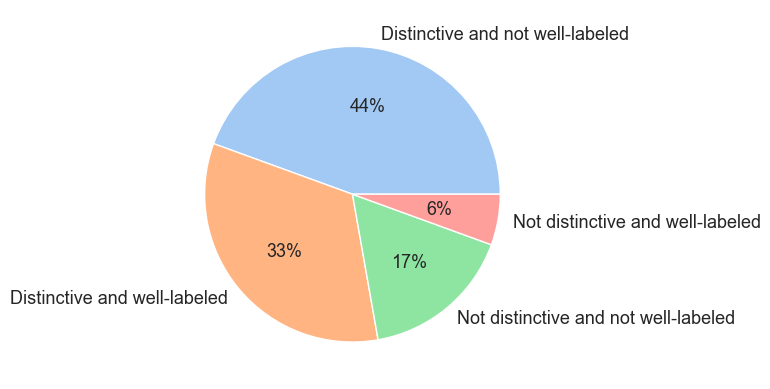
\includegraphics[width=.8\textwidth]{images/subplots/rating_piecharts.png}
	\caption[Sub-topic clustering output feedback.]{Piechart detailing the feedback on the sub-topic clustering output. \label{fig:question_1_piechart}}
\end{figure}

The user feedback is further analyzed individually and shared in \prettyref{fig:question_1_barplot}. Fourteen survey inputs agree with the distinctiveness of the sub-topics, and four inputs share contrary feedback, i.e., non-distinctive. Similarly, 11 user inputs show that the cluster labels or sub-topic names need to be better labeled, and seven inputs show the opposite pattern.

\begin{figure}[h]
	\centering
	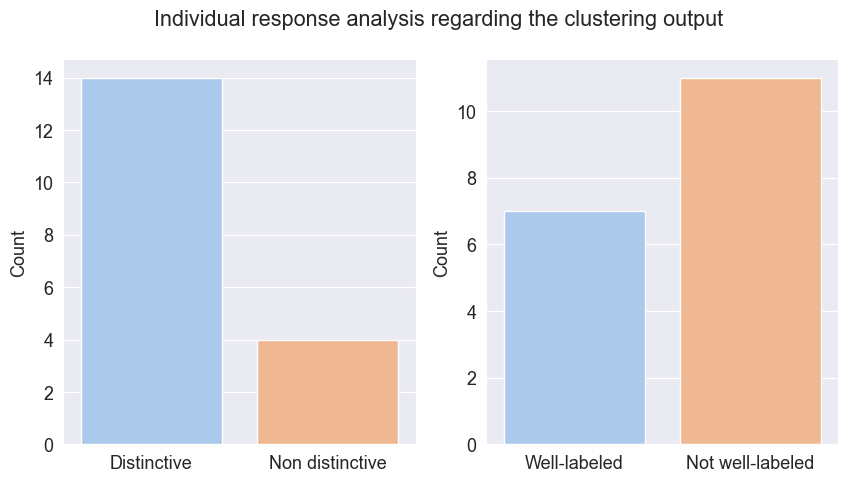
\includegraphics[width=.9\textwidth]{images/subplots/barplots.png}
	\caption{Barplot highlighting the individual response.  \label{fig:question_1_barplot}}
\end{figure}


It is evident from the above table that most of the survey participants agree with the distinctiveness of the sub-topics. Therefore, the candidate keyword selection positively impacts the clustering by creating distinctive clusters. However, the sub-topic labeling approach that uses the clusters' centroid needs to generate better results. After analyzing the sub-topic labels from \prettyref{tab:65_output} and \prettyref{tab:5G_output}, it can be observed that some of the sub-topics have abbreviations as labels. For example, DAQC, ATT, UMTS, etc., are some labels that might not be familiar to many participants and can lead to poor interpretation of the cluster and its documents.

\subsection{System Comparison Response Analysis}

These questions are targeted to evaluate the two IR systems developed to represent the retrieved documents. System A retrieves news-articles using the sub-topic modeling output and re-ranks them using a dynamic template, while System B retrieves news-articles with a new query request to the semantic index using the same template. Furthermore, quantitative ratings ranging from 0 to 10 are collected for both systems. Some participants have provided false inputs, and these inputs are considered anomalies. These anomaly feedback inputs for questions 2, 3, and 4 are removed from the analysis. One such feedback is observed and shared in \prettyref{tab:question_234_anamoly}. It is clear that the user has provided a lower rating for System B than for System A. However, the user has chosen System B as the better system, which clearly contradicts the individual ratings.


 \begin{center}
	\captionof{table}{Improper user feedback input in the survey. }\label{tab:question_234_anamoly}
	\begin{tabularx}{.8\textwidth}{|Y|c|c|}
		\hline
		Which IR system is better? & System A ratings & System B ratings \\
		\hline
		\ac{System B} & 10 & 6.1 \\
		\hline
	\end{tabularx}
\end{center} 

Participants are requested to answer a qualitative comparison between the two systems, and the results are shared in \prettyref{tab:question_2_results}. After removing the anomalies, it is evident from \prettyref{tab:question_2_results} that most participants have agreed that System A retrieves documents better than System B. This result is derived from the qualitative inputs of the survey. However, it is crucial to determine the significance of this result through the quantitative inputs, i.e., system ratings.

\begin{center}
	\captionof{table}{Question 2, 3, and 4 results.}\label{tab:question_2_results}
	\begin{tabular}{ cc }   % top level tables, with 2 columns
		IR system comparison  & Questions 3 and 4 \\  
		% leftmost table of the top level table
\begin{tabularx}{.4\textwidth}{|Y|c|}
	\hline
	Label & Count \\
	\hline
	System A & \textbf{18} \\
	\hline
	System B & 0 \\
	\hline
	Neither System A nor System B & 4 \\
	\hline
	
\end{tabularx} &  % starting rightmost sub table
		% table 2
		\begin{tabularx}{.45\textwidth}{|c|c|Y|Y|}
			\hline
			System & Mean & Standard deviation & Variance \\
			\hline
			 A & \textbf{5.46} & 2.92  & 8.54 \\
			\hline
			 B & 3.28 & 2.77 & 7.7 \\
			\hline

		\end{tabularx} \\
	\end{tabular}
\end{center}

\prettyref{tab:question_2_results} shows that System A has a better mean than System B, and there is no significant difference in the standard deviation. Individual system ratings are plotted in a histogram and presented in \prettyref{fig:histograms}. These distributions clearly show that System B ratings are more concentrated towards lower values and follow a right-skewed distribution. On the other hand, System A ratings are not concentrated at a certain level but rather follow a positive trend with some high ratings.

\begin{figure}[h]
	\centering
	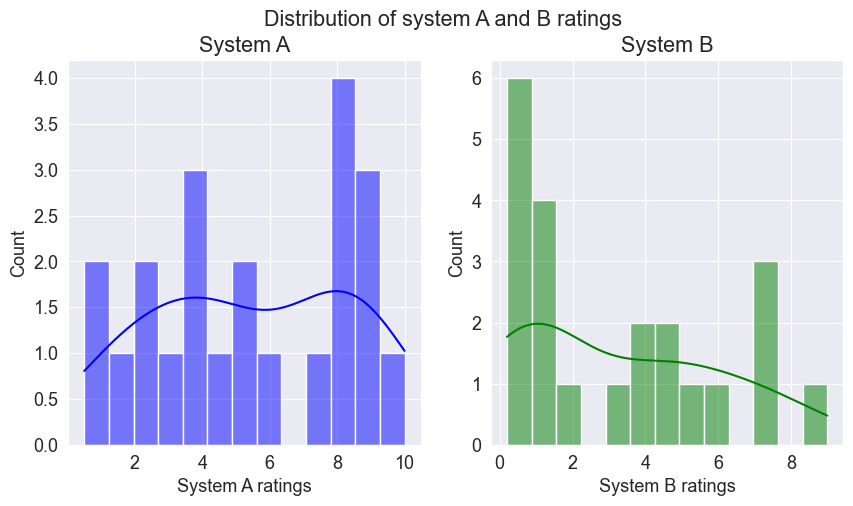
\includegraphics[width=.99\textwidth]{images/subplots/rating_histograms.png}
	\caption{Histograms showing the distribution of system ratings.  \label{fig:histograms}}
\end{figure}



The significance of one system performing better than the other can be evaluated with the help of statistical testing. The system ratings are collected for two systems for a given query and sub-topic. Therefore, the sample data can be considered as paired data as they are relative to each other and not compared with other queries or sub-topics. This relation between the data is also referred to as dependent data samples. \prettyref{fig:histograms} shows that the system ratings do not follow any specific distributions, and therefore, parametric statistical tests are not feasible. A non-parametric hypothesis test, namely the \emph{Wilcoxon signed-rank test}~\cite{buWilcoxonSigned}, is chosen in this master's thesis. This statistical test considers the signs of the difference scores between the dependent data along with the magnitude of the differences. In the Wilcoxon Signed Rank Test, the hypothesis is built on the median of the difference scores~\cite{buWilcoxonSigned, kaur2015comparative}.


\begin{enumerate}
	\item \textbf{Null Hypothesis ($H_0$)}: The median difference between the samples, namely "System A" and "System B" ratings is zero.
	
	\item \textbf{Alternate Hypothesis ($H_1$)}:  The median difference between the samples, namely "System A" and "System B" ratings is not zero.
\end{enumerate}

The hypothesis is based on whether the median difference is equal to zero or not, rather than being compared to a specific value. Thus, this is referred to as a two-tailed test. Before performing the statistical testing, it is crucial to choose the confidence level and the test statistic. A confidence level of 95\% is chosen, i.e., a significance level ($\alpha$) of 0.05, and for the test statistic, the z-score is selected. \prettyref{fig:z_score} shows the acceptance and rejection regions for the significance level $\alpha$ = 0.05. If the test score is lower than -1.96 or greater than 1.96, the null hypothesis should be rejected, and the alternative hypothesis should be accepted. In any other case, the null hypothesis must be accepted.


\begin{figure}[h]
	\centering
	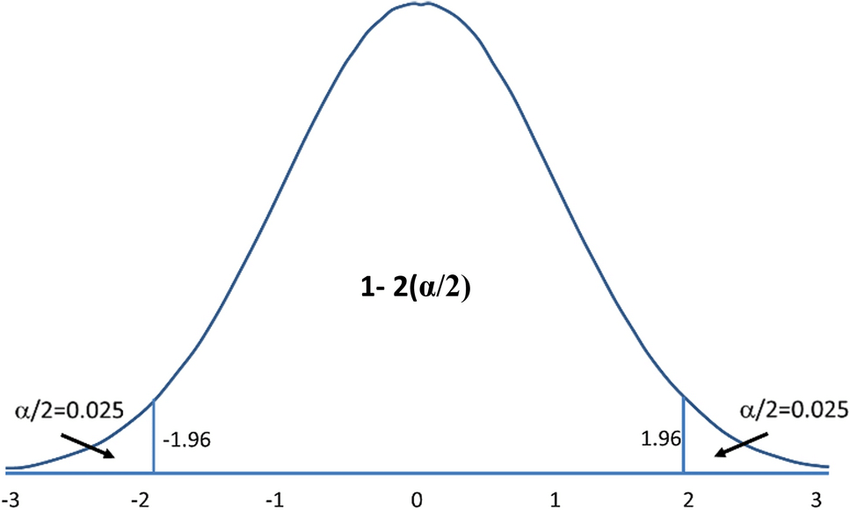
\includegraphics[width=.75\textwidth]{images/outside/z_score.PNG}
	\caption[Rejection regions for z test-statistic.]{Rejection regions for a significance level of 0.05 and z test-statistic. \cite{article} \label{fig:z_score}}
\end{figure}



The test statistic is calculated using the python library \textit{researchpy}\footnote{\url{https://researchpy.readthedocs.io/en/latest/index.html}}. The calculated z-score is 4.06, and the test score is larger than the critical value of 1.96. Therefore, the null hypothesis is rejected, and the alternative hypothesis is accepted. This means that the system ratings are significantly different, and System A retrieves better news-articles related to the user query and the sub-topic. This concludes the system comparison by suggesting that retrieval using the sub-topic modeling output has performed better than a new query retrieval for a given query and sub-topic.

\subsection{System Comparison Query Analysis}

The system comparison is statistically evaluated, with the conclusion that System A represents the news-articles better based on the sub-topic clustering output. However, the mean system A ratings from the participants are around 5.46, which is not high on a scale of 10. From \prettyref{fig:histograms}, it is evident that a few responses for System A are high, while the other ratings are very low. To understand the user responses, the high and low ratings of System A are analyzed. The query and sub-topics used for System A are presented in \prettyref{tab:queries_question_234}.

\begin{center}
	\captionof{table}{Query and sub-topic analysis for system A. }\label{tab:queries_question_234}
	\begin{tabular}{ cc }   % top level tables, with 2 columns
		Top-25 percentile ratings & Bottom-25 percentile ratings \\  
		% leftmost table of the top level table
		\begin{tabularx}{.4\textwidth}{|Y|Y|}
			\hline
			Query  & Sub-topic \\
			\hline
			Künstliche Intelligenz & KI  \\
			\hline
			Künstliche Intelligenz & Military \\
			\hline
			Kryptographie & \textbf{Polizei Geheimdienst}\\
			\hline
			china Image recognition & Privacy \\
			\hline
		\end{tabularx}&  % starting rightmost sub table
		% table 2
		\begin{tabularx}{.55\textwidth}{|Y|c|}
			\hline
			Query  & Sub-topic \\
			\hline
			Main Ground Combat System & \textbf{Projekt}  \\
			\hline
			Main Ground Combat System & Laser beam \\
			\hline
			Edge computing & \textbf{SOSA} \\
			\hline
			Edge computing & Everbetter processor \\
			\hline
			Geoinformationen & \textbf{Operationsführung} \\
			\hline
			Semantische Technologien & \textbf{March} \\
			\hline
		\end{tabularx}\\
	\end{tabular}
\end{center}

From the bottom 25 percentile System A ratings, it can be observed that the sub-topics chosen for retrieving news-articles are unusual and not well related to the query. For example, the sub-topic \textit{Projekt} is too generic for a military query keyword such as \textit{Main Ground Combat System}. Similarly, the sub-topics \textit{March, SOSA, Operationsführung} lead to poor results as they do not effectively represent the sub-topic clusters. This pattern aligns with earlier observations where the majority of participants chose 'Not well-labeled' for the sub-topics. The sub-topic labeling is created using a centroid-based approach, which assigns the keyword closest to the centroid as the label of the cluster, disregarding key criteria such as abbreviations, understandability, uniqueness, etc.

\subsection{Subtopic Retrieval Response Analysis}

Participants are requested to share feedback on finding relevant documents using the proposed approach. The actual question asked in the survey is "Were the sub-topics helpful for you to find the relevant documents?". There are only two options to answer this question: 'Yes' or 'No'. The results show that around half of the participants found that the approach of retrieving documents using sub-topics does not help find news-articles related to innovation.

\mycomment{One drawback of this question is that it does not specify
	the particular IR system. This can lead the users to provide biased input during the survey.
	To overcome this, two questions specific to two systems (A and B) should have been asked to the
	participants.}


\begin{center}
	\captionof{table}{Question 5 results.}\label{tab:question_5_results}
	\begin{tabularx}{.3\textwidth}{|Y|c|}
		\hline
		Label & Count \\
		\hline
		Yes & 6 \\
		\hline
		No & 5 \\
		\hline
	\end{tabularx}
\end{center} 

One reason for this could be the lack of relevant documents in the database for a particular query and sub-topic. Another reason could be the need for participants to assess the relevance of the retrieved documents, as the expected number of relevant documents might be low. Assuming these cases are different from the ones observed here, the proposed approach did not successfully assist the users in finding the relevant documents. On the other hand, participants who found it helpful suggest the possibility of using this approach to find relevant documents.

\subsection{Subtopic Retrieval Query Analysis}

The user queries collected for the sub-topic retrieval question are analyzed and shown in \prettyref{tab:queries_question_5}. The queries are divided into two categories: 'Yes' or 'No', based on the participants' responses. It is observed that the participants have provided positive feedback for search queries related to technology. On the other hand, there are only two queries related to military, such as \emph{Main Ground Combat System} and \emph{Geoinformationen}, and they have received negative feedback. This indicates that the users are not satisfied with the retrieved results for military-related queries.

\begin{center}
	\captionof{table}{Queries collected for the subtopic retrieval effectiveness.}\label{tab:queries_question_5}
	\begin{tabularx}{.8\textwidth}{|Y|Y|}
		\hline
		Yes & No \\
		\hline
		Künstliche Intelligenz  & \textbf{Main Ground Combat System} \\
		\hline
		Mobile Kommunikation & \textbf{Geoinformationen} \\
		\hline
		Quantentechnologie & \textbf{Edge computing} \\
		\hline
		Kryptographie & \textbf{Semantische Technologien} \\
		\hline
		china Image recognition & Robotik \\
		\hline
	\end{tabularx}
\end{center} 

One possible reason for the queries receiving negative feedback is the sub-topic selected by the participants. This can be observed from \prettyref{tab:queries_question_234} for the queries \emph{Edge computing} and \emph{Semantische Technologien}. However, the sub-topic information is not collected during the assessment of sub-topic retrieval effectiveness. Therefore, it cannot be determined whether the choice of sub-topic is the reason for the poor retrieved results.


\section{Precision Analysis Results}

This section details the results of the exploratory analysis on the ranking of sub-topics and the documents within those sub-topics. These rankings aim to generate a unique series of retrieved documents that simulate the user's real-time traversal. The description of the \ac{IR} systems developed in this master thesis is shared in Section 6.6 and briefly presented again in \prettyref{tab:ir_system_intro}. Two evaluation metrics, namely mean expectation score and mean average precision, are used to evaluate the ranking output. Only a small candidate pool (CP-30) is used for this analysis, as labeled data is required to calculate the mean expectation and precision scores.


\begin{center}
	\captionof{table}{Brief IR system introduction.}\label{tab:ir_system_intro}
	\begin{tabularx}{0.8\textwidth}{|c|Y|Y|}
		\hline
		IR system name & Sub-topic ranking & Document ranking \\
		\hline
		IR0 & NA & Uniform distribution  \\
		\hline
		IR1 & NA & Query similarity \\
		\hline
		IR2 & Query similarity & Query similarity \\
		\hline
		IR3 & Template similarity & Template similarity \\
		\hline
		IR4 & Document cardinality & Query similarity \\
		\hline
		IR5 & (IR4, IR2) &  Query similarity \\
		\hline
		IR6 & (IR4, IR2, IR3) & Query similarity \\
		\hline
		IR7 & Random combinations & Query similarity  \\
		\hline
	\end{tabularx}
\end{center}

\subsection{Mean Expectation Score Analysis}

Expectation scores are calculated at a specific index, indicating the number of relevant documents. This analysis utilizes the mean expectation score, averaged over the 17 queries in the testset. For instance, a mean expectation score ($ME_5$) of 2 at index 5 signifies that, on average, there are two relevant documents among the top 20 retrieved documents. The higher the mean expectation score of an \ac{IR} system, the better the retrieval performance. This analysis is crucial for users interested in reading documents at a specific index, allowing them to choose the best \ac{IR} system accordingly.

\begin{figure}[h]
	\centering
	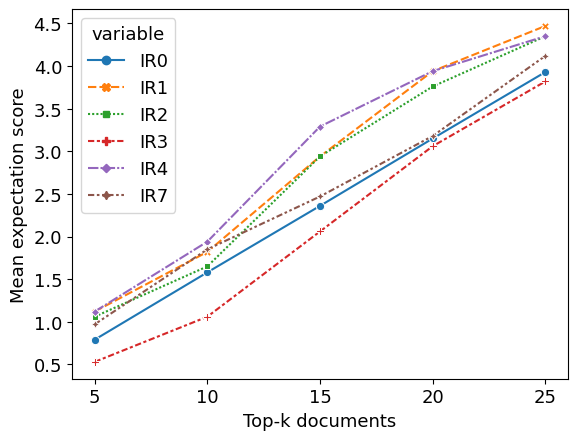
\includegraphics[width=.85\textwidth]{images/subplots/mean_expectation_score.png}
	\caption{Mean expectation score plot. \label{fig:mae_fig}}
\end{figure}

\prettyref{fig:mae_fig} presents the mean expectation score of six \ac{IR} systems across five retrieval indices. Combinational IR systems, namely IR5 and TR6, are excluded from this plot as their results were similar to IR4 and thus redundant. One notable observation from \prettyref{fig:mae_fig} is that the IR4 system, which employs template similarity, performs poorly compared to the other IR systems. The same retrieval technique is used in the survey. The remaining IR systems exhibit similar patterns and are closely related. At index 15, the IR4 system, utilizing document cardinality, demonstrates relatively better performance than the other retrieval systems.


\begin{center}
	\captionof{table}{Mean expectation score results.}\label{tab:mae_results}
	\begin{tabularx}{0.8\textwidth}{|Y|c|c|c|c|c|}
		\hline
		IR system name & ME@5 & ME@10 & ME@15 & ME@20 & ME@25 \\
\hline
IR0 &          0.79 &           1.58 &           2.36 &           3.15 &           3.93 \\ \hline 
IR1 &          \textbf{1.12} &           1.82 &           2.94 &          \textbf{3.94} &           \textbf{4.47} \\ \hline
IR2 &          1.06 &           1.65 &           2.94 &           3.76 &           4.35 \\ \hline
IR3 &          0.53 &           1.06 &           2.06 &           3.06 &           3.82 \\ \hline
IR4 &           \textbf{1.12}  &            \textbf{1.94}  &          \textbf{3.29} &           \textbf{3.94} &           4.35 \\ \hline
IR5 &           \textbf{1.12}  &           \textbf{1.94} &           \textbf{3.29} &       \textbf{3.94}&           4.41 \\ \hline
IR6 &          \textbf{1.12}  &           \textbf{1.94} &           \textbf{3.29} &           3.88 &           4.41 \\ \hline
IR7 &          0.97 &           1.85 &           2.47 &           3.18 &           4.12 \\ \hline
	\end{tabularx}
\end{center}

\prettyref{tab:mae_results} displays the detailed expectation scores of the \ac{IR} systems. Among the baseline systems, IR1, which does not utilize clustering, performed the best at the 25th retrieval index. However, the other \ac{IR} systems, including IR7, which employs random combinations, exhibited better performance compared to the baseline systems IR0 and IR1. This clearly indicates that sub-topic clustering does not deteriorate the order of relevant documents as the user traverses through the sub-topics. Additionally, users benefit from the ability to select a specific sub-topic and directly access the relevant documents, enhancing retrieval efficiency.

\subsection{Mean Average Precision Analysis}

Mean average precision (MAP) provides a concrete score for comparing different \ac{IR} systems based on the retrieved documents. Without specific index analysis, the \ac{IR} system with the highest MAP score can be identified as the best \ac{IR} system. \prettyref{tab:map_results} presents the \ac{MAP} scores of the \ac{IR} systems. Similar to the mean expectation scores, the IR3 system, which employs template similarity, performs poorly compared to other systems. Despite having the highest MAP score, the combination systems IR5 and IR6 do not demonstrate any improvement in retrieval performance. Combining multiple sub-topic rankings to generate a unified document ranking could yield more successful results, with one main reason being the need for a greater count of relevant documents.


\begin{center}
	\captionof{table}{Mean average precision results.}\label{tab:map_results}
		\begin{tabularx}{0.4\textwidth}{|c|Y|}
		\hline
		IR system name & MAP \\
		\hline
		IR0 & 0.185 \\
		\hline
		IR1 &  0.3 \\
		\hline
		IR2 &  0.303 \\
		\hline
		IR3 &  0.198 \\
		\hline
		IR4 &   \textbf{0.316} \\
		\hline
		IR5 &    \textbf{0.316} \\
		\hline
		IR6 &   0.315\\
		\hline
		IR7 &  0.292 \\
		\hline
	\end{tabularx}
\end{center}


The IR7 system, utilizing random combinations of sub-topic clusters, achieves a significant score and performs better than the baseline IR0. A simple document ranking based on query similarity without sub-topics (i.e., IR1) performs similarly to the IR2 system, which incorporates sub-topic ranking. This indicates that the retrieval performance remains consistent even with the introduction of sub-topics. Furthermore, the IR4 system, which utilizes document cardinality as the ranking criterion, performs the best. Although the difference is not significantly higher than other systems, IR4 possesses an inherent advantage over the baselines IR0 and IR1 in terms of accessing documents within a specific sub-topic.

\subsection{Ineffectiveness of Combinational IR systems}

Combinational \ac{IR} systems, namely IR5 and IR6, have shown no significant improvement in performance. From the analysis results in \prettyref{tab:mae_results} and \prettyref{tab:map_results}, the combinational systems perform equally well or lower compared to the individual systems, such as IR4, which is based on document cardinality. The poor performance is due to the ineffectiveness of the algorithm in ranking positive documents at the top of the retrieved results. Retrieval performance is directly dependent on document ranking, which can be observed through MAP or MAE. These metrics are also greatly influenced by the number of positive documents, and it has been observed that the number of positive documents in the testset is relatively low.

Nevertheless, the effectiveness of the algorithm in generating combinational \ac{IR} systems is evaluated by finding the unique document list generated through retrieval. To perform this analysis, two metrics are proposed: $R_s$, the number of unique sub-topic rankings, and $R_d$, the number of unique document rankings. Here, a unique ranking refers to a document or sub-topic ranking that differs from the rankings generated by the IR4 system. Generating new sub-topic and document rankings does not necessarily indicate better retrieval performance. However, it can reveal the effectiveness of the algorithm in generating new ranking patterns by combining ranking information from individual retrieval systems. These metrics are calculated as aggregate functions over 17 different queries in the testset. Therefore, the maximum possible value for these metrics is 17, and the minimum possible value is 0. Both large and small candidate pools are considered in this analysis.

\begin{center}
	\captionof{table}{Unique ranking counts of sub-topics and documents.}\label{tab:unique_ranking_counts}
	\begin{tabular}{ cc }   % top level tables, with 2 columns
		CP - 30 & CP - 100 \\  
		% leftmost table of the top level table
		\begin{tabularx}{.35\textwidth}{|Y|c|c|}
			\hline
			IR system name & $R_s$ & $R_d$ \\
			\hline
			IR5 & 15 & \textbf{8} \\
			\hline
			IR6 & 15 & \textbf{10} \\
			\hline
			
		\end{tabularx} &  % starting rightmost sub table
		% table 2
		\begin{tabularx}{.35\textwidth}{|Y|c|c|}
	\hline
	IR system name & $R_s$ & $R_d$ \\
	\hline
	IR5 & 17 & 17 \\
	\hline
	IR6 & 17 & 17 \\
	\hline
			
		\end{tabularx} \\
	\end{tabular}
\end{center}

\prettyref{tab:unique_ranking_counts} shows the unique ranking lists generated by the systems IR5 and IR6. In the case of CP-30, it is evident that the number of unique sub-topic rankings $R_s$ for both IR5 and IR6 is 15, which is close to the maximum value. This shows that in most of the queries, a new sub-topic ranking is created. However, the unique document rankings $R_d$ are 8 and 10 for IR5 and IR6 respectively. This shows that almost half of the new rankings generated by the combinational systems are redundant, resulting in no significant improvement in the performance. In the case of CP-100, the combinational systems generate unique sub-topic and document rankings for every query. This signifies the possibility of evaluating more patterns and having better performance.

\subsection{Literature Comparison Results}



The proposed approach in this master thesis is compared against the literature, which is detailed in Section 6.6.3. Three retrieval techniques are considered to create candidate documents for re-ranking, and two ranking approaches are used to generate the final ranking list of news-articles. To evaluate the performance of retrieval, mean average precision (MAP) is used, and a higher score signifies better retrieval performance of the IR system. From \prettyref{tab:map_results}, it is evident that IR4, the system that uses document cardinality for sub-topic ranking and query similarity for document ranking, has shown the best results. The same system is used for sub-topic retrieval and compared with the cross-encoder ranking. \prettyref{tab:literature_results} shows the evaluation results of the proposed approach compared to the literature.

\begin{center}
	\captionof{table}{Literature comparison results.}\label{tab:literature_results}
	\begin{tabularx}{0.8\textwidth}{|Y|Y|c|}
		\hline
		Retrieval technique & Re-ranking technique & MAP \\
		\hline
		BM-25 retrieval & Cross-encoder ranking & \textbf{0.171}  \\
		\hline
		BM-25 retrieval  & Sub-topic retrieval & 0.114 \\
		\hline
		\hline
		Bi-encoder retrieval  & Cross-encoder ranking & \textbf{0.132} \\
		\hline
		Bi-encoder retrieval  & Sub-topic retrieval & 0.081 \\
		\hline
		\hline
		Candidate pool retrieval  & Cross-encoder ranking & 0.174 \\
		\hline
		Candidate pool retrieval & Sub-topic retrieval &  \textbf{0.265} \\
		\hline
	\end{tabularx}
\end{center}


It is observed that the sub-topic retrieval, along with the candidate pool retrieval, has performed the best out of all scenarios with a \ac{MAP} score of 0.265. Moreover, the cross-encoder ranking approach has achieved the best \ac{MAP} score when the candidate pool is used at the retrieval stage. This clearly shows that a candidate pool, which is a mixture of lexical and semantic matching, has generated better results than the other retrieval techniques. In this master thesis, efforts are made to select the significant candidate document set using an optimized candidate pool selection strategy. The \ac{MAP} score of the sub-topic retrieval approach with document cardinality and query similarity from \prettyref{tab:literature_results} is lower than in \prettyref{tab:map_results}. The reason for this difference, despite the usage of the exact approach, is the candidate pool. In the literature comparison, a large candidate pool of 100 documents is used rather than the small candidate pool.

On the other hand, the cross-encoder ranking technique showed better retrieval performance in the case of BM-25 and bi-encoder retrieval output. This shows that the overall performance of the cross-encoder is better than sub-topic retrieval. However, in the case of sub-topic retrieval, the user can access the news-articles from a certain topic easily with a single click. In order to extract diverse sub-topics and access several news-articles, a large candidate pool retrieval is suggested with sub-topic retrieval. The effectiveness of the cross-encoder can be used within sub-topic retrieval. For example, the document ranking in sub-topic retrieval can possibly be replaced with cross-encoder ranking instead of query similarity ranking.


 



    
        % !TEX root = ../thesis.tex

\chapter{Conclusion}

This master thesis analyzes the challenges involved in retrieving relevant long text documents, such as news articles, for a short keyword query. The proposed approach is evaluated in this study. This pivotal chapter provides a concise summary of the master thesis and highlights a few limitations encountered during the experiment. The chapter is divided into three sections: \textit{Thesis Summary}, \textit{Limitations}, and \textit{Future Work}. The Thesis Summary section compiles essential details from all chapters within the master thesis. The \textit{Limitations} section emphasizes the inherent drawbacks in the proposed approach and underscores potential threats to the validity of our experimental outcomes, ensuring a critical evaluation of the experiment results. The \textit{Future Work} section outlines suggestions to enhance the proposed approach and outlines steps to extend the current research.

\section{Thesis Summary}

The objective of this master thesis was to assess the impact of a candidate keyword selection approach in generating diverse sub-topics during the retrieval of long text documents. The experiment consisted of two stages: evaluating the effectiveness of the candidate keyword selection approach and examining the potential of the selection technique to improve retrieval performance. Additionally, the thesis extends its evaluation through exploratory analysis and literature comparison. The thesis addresses three research questions: RQ1, RQ2, and RQ3. To begin, the thesis introduces the existing work, which is an information retrieval (IR) system initially developed for retrieving news articles at \ac{FKIE}. 

The essential details regarding the \ac{IR} system, such as the process of downloading news articles, their classification, and storage in document indices, are briefly described. The \ac{IR} system employed in this research utilizes lexical and semantic matching algorithms to retrieve relevant news articles based on user search queries. However, the search experience of this system was significantly affected when faced with short queries and lengthy text documents. To address this challenge, a novel approach was proposed in this master thesis to efficiently extract topic representations, specifically subtopics, from the retrieved documents.

After conducting an extensive literature review, a pipeline was developed to carefully select specific keywords that would be instrumental in generating diverse subtopics for a given search query. This selection technique, referred to as \textit{Candidate Keyword Selection}, serves as the central and distinguishing component of the proposed pipeline. Furthermore, an optimized candidate document pool was created to incorporate more representative documents related to the user's query. Essentially, subtopics are derived through term-based clustering of the candidate documents, and experiments were conducted to evaluate the significance of these diverse subtopics on retrieval performance.


RQ1 focuses on evaluating the results of the sub-topic extraction pipeline by employing two target functions on two candidate pools. One of the target functions used is the \textit{Silhouette index}, which assesses the distinctiveness of the generated sub-topics. However, it was observed that this metric failed to capture the diversity of clusters, as it solely relied on the separation between clusters without considering their semantic nature. The second target function, called the \textit{Targeted Negative Document Ratio}, utilizes labeled test set information to determine the distinctiveness of sub-topics. This function performed well when labels were available for all documents in the candidate pool i.e. CP-30. However, due to the lack of labels in the large candidate pool, this evaluation metric proved ineffective. As a result, a manual parameter selection approach was adopted, and the pipeline parameters were finalized based on this process. 

RQ2 expands the evaluation of the sub-topic outcomes and their significance through the use of a survey questionnaire. A dedicated website was developed for survey participants to interact with the sub-topic retrieval system and assess its effectiveness in retrieving relevant news articles, specifically those related to innovation, for a given search query. The feedback from the survey indicated that the generated sub-topics through the proposed approach were distinct from each other. However, the majority of participants expressed that the sub-topics were poorly labeled. Additionally, a quantitative comparison was conducted between two \ac{IR} systems. The first system, \textit{System A}, utilized the sub-topic modeling output, while the other system, \textit{System B}, used a newly generated query through a dynamic template.

The survey results statistically determined that \textit{System A} performed better in retrieving news articles for a given query and sub-topic. However, upon careful analysis of \textit{System A}'s results, it was observed that the poor retrieval outcomes were due to the choice of sub-topic being completely irrelevant to the query. Furthermore, one of the survey questions focused on whether the sub-topics truly helpful to users in finding relevant news articles. The feedback to this question revealed that nearly half of the participants found the retrieval process with sub-topics to be beneficial.

RQ1 and RQ2 focused on evaluating sub-topic generation, while RQ3 assessed the retrieval performance for various combinations of sub-topic ranking and document ranking pairs using the Mean Average Precision (MAP) metric. Eight different \ac{IR} systems, ranging from IR0 to IR7, were proposed and compared against each other. The \ac{IR} system that performed the best was then compared with the existing literature. Among the IR systems, IR4 exhibited the highest \ac{MAP} results. IR4 utilized sub-topic ranking based on the decreasing order of the number of documents within each cluster, combined with document ranking based on decreasing query similarity. The retrieval performance of the IR4 system was compared to literature that employed a \textit{Cross-encoder} for generating ranked results. Both approaches utilized a multi-stage ranking architecture.

At the first stage, three different retrieval approaches, namely \textit{BM-25, Bi-encoder, and Candidate pool}, were used to retrieve candidate documents. In the second stage, the IR4 system approach was compared to the cross-encoder using \ac{MAP} as the evaluation metric. The results of the comparison indicated that the IR4 ranking approach performed the best when using the candidate pool as the retriever. However, the cross-encoder generated better rankings of news articles when candidate documents were retrieved using BM-25 and bi-encoder.

\section{Limitations}

The primary objective of the target users at \ac{FKIE} is to explore news articles related to innovation in the military and technology fields. The candidate keyword selection method proposed in the master thesis relies solely on query similarity to choose keywords that can generate diverse sub-topics. However, one limitation of this approach is that it does not directly address the retrieval of innovation-related documents; instead, it focuses on segmenting the documents into clusters.

Additionally, relying solely on one feature, namely query similarity, for keyword selection is not ideal and may result in inefficient keyword selection. The context-based keyword extraction technique employed in this approach selects the top 25 noun chunks as keywords but ignores their relevance distribution within the news article. The true potential of the proposed approach is explored when all noun chunks are considered as candidate keywords, although this may introduce computational challenges. Nonetheless, selecting specific noun chunks based on their importance in a news article, considering their distribution, could help mitigate this drawback.


The absence of sub-topic labels in the test set has necessitated the selection of pipeline parameters using intrinsic and extrinsic cluster evaluation approaches. However, the chosen target functions for parameter selection have revealed a lack of effectiveness in capturing distinctiveness, leading to the need for manual parameter selection. The limitations of the employed target functions in the master thesis are discussed in Section 7.1.6. Manual parameter selection introduces the risk of human bias and proves highly inefficient, particularly when dealing with a large number of parameters. To optimize sub-topic extraction, the thesis implemented the caching of keyword embeddings, resulting in an average real-time extraction time of 7.75 seconds. Although this optimization has reduced extraction time, it is important to note that compared to current search engines, which often deliver results in just a few seconds, the sub-topic retrieval approach remains relatively slower. This difference in speed may potentially impact user satisfaction negatively.

The survey questionnaire and its evaluation are subject to certain limitations. While the survey participants are randomly selected regardless of their background, they may not fully represent the target users, introducing the possibility of non-representative sample bias. Another limitation arises from the lack of explicit definitions for certain queries or phrases used in the questionnaire, such as "Distinctive," "Well-labeled," "IT-Bedrohungsanalyse," "Unbemannte Landsysteme," and so on. Although these terms may seem self-explanatory, they can still be subject to interpretation by participants who are unfamiliar with these phrases in both German and English.

Additionally, the survey question assessing the usefulness of sub-topic retrieval does not gather system and sub-topic information from the participants. This missing information creates the potential for response bias, and the analysis of this specific question in the survey cannot be fully justified.

\section{Future Work}

To effectively address innovation-related news articles, the distinctive sub-topics extracted through the proposed approach in the master thesis can be further expanded to include sub-topic classification. By tracking user information from the sub-topic retrieval system, it becomes possible to observe which sub-topics are of high interest to users. This differentiation among sub-topic clusters proves valuable in identifying and eliminating non-innovation-related clusters. Instead of solely relying on the similarity between keywords and the search query, the candidate keyword selection technique can incorporate additional information related to technology, military, security, and other relevant domains. Integrating these features enhances the criteria for keyword selection and also improves the output of sub-topic clustering.

In the present research, it has been observed that the silhouette score is not effective in capturing the distinctiveness of the cluster output, despite the clustering demonstrating better separation. Further investigation is required to develop an efficient evaluation metric that can assess the distinctiveness of sub-topics considering semantic information. Additionally, there is room for further optimization of sub-topic generation to reduce the average extraction time from 7.75 seconds to less than 2 seconds. Based on the evaluation from the survey, it has been determined that the sub-topics are not well-labeled. This highlights the need for improvement in the naming of clusters using the cluster centroid technique, or the exploration of more robust techniques for labeling.

This master thesis utilized the \ac{USE} at multiple stages within the proposed approach to encode the query, noun phrases, and news articles. However, since the completion of this research, several more efficient and state-of-the-art sentence encoding models have been published. It is imperative to evaluate the current research using these newly developed models to ensure its performance remains up-to-date.

Additionally, the performance of the multi-stage ranking architecture employed in this research should be evaluated against the recent advancements made in \textit{\ac{LLM}}. Unlike the approach used in this thesis, where relevant documents are extracted for a given query, \ac{LLM}s focus on generating relevant answers directly from the knowledge source. Furthermore, \ac{LLM}s have the potential to be utilized for generating sub-topics, thereby providing an alternative to the traditional topic modeling or clustering approach.





    % Literaturverzeichnis
       \printbibliography[heading=bibintoc]
 

   % !TEX root = ../thesis-sample.tex
\appendix
%\doublespacing
\chapter{Technical keywords and definitions}
\label{appendix:A}
\begin{description}
	
	
		\item[Bootstrap] \hfill \\ Bootstrap is an open-source \ac{CSS} framework for developing responsive websites~\cite{simplilearnWhatBootstrap}.
	Responsive websites look alike when tested in different environments, such as device screen sizes and orientations (portrait/landscape). The website
	used in the survey questionnaire is developed using Bootstrap.
	
	\item[Context] \hfill \\ In this master thesis, context is defined as a particular domain or field in which the user is interested. For example, in the user query \emph{Cloud}, the retrieved documents are related to different domains or contexts, such as cloud computing, combat cloud, and clouds in the sky. Even though there is some syntactic and semantic matching, the user intention is still unclear from the query.

		\item[Cosine similarity] \hfill \\     Cosine similarity is a metric to measure the degree of similarity between two vectors~\cite{lahitani2016cosine}. In the case of IR systems, the similarity is calculated between the user query and document sentence embeddings, and can be further used to rank the documents.
		
		
		 \item[CSS] \hfill \\ 
	
	\ac{CSS} is a rule-based language for styling websites~\cite{mozillaWhatCSS}. The elements in a website can be placed appropriately using specific rules mentioned in \ac{CSS}. Furthermore, many front-end visual features, such as text size, color, animations, etc., can be configured using \ac{CSS}.
	
		\item[Docker] \hfill \\ Docker is an open-source technology that allows developers to build, test and
	deploy their software applications efficiently. Docker uses container technology, software that bundles the code and its dependencies to run the applications seamlessly~\cite{dockerWhatContainer}. Containers virtualize the operating
	system independent of the hardware, which creates better code reproducibility.  
	
		\item[Extrinsic evaluation] \hfill \\ In \emph{Extrinsic evaluation}, the clustering output is evaluated using the external knowledge such as ground-truth or the relevance judgments~\cite{de2012document}. 
		
		
		\item[FastAPI] \hfill \\ FastAPI\footnote{\url{https://fastapi.tiangolo.com/lo/}} is a Python-based web framework for building APIs used as a
	backend or server-side technology. The survey questionnaire developed in this master thesis is
	developed using FastAPI.
	
		\item[Fuzzy string matching] \hfill \\ Fuzzy string matching is a string matching technique that identifies how approximately two strings are similar. In lexical matching, the outcome of string matching follows a binary outcome of similar or not similar. In fuzzy matching, the individual parts of the text are considered to generate an approximate string similarity score. This approximate string matching is beneficial in information retrieval when certain words are misspelled in the user query~\cite{redisWhatFuzzy}.
		
			 \item[FuzzyWuzzy] \hfill \\ FuzzyWuzzy\footnote{\url{https://pypi.org/project/fuzzywuzzy/}} is an open-source library in Python to calculate the syntactical text similarity between two strings. Internally, the library uses levenshtein distance. FuzzyWuzzy assigns a score between 0 and 100 according to the similarity between two strings.
			 
	\mycomment{	\item[Ground-truth] \hfill \\
		
		Ground-truth labels are information that is more accurate, relevant, and true than the knowledge of the system being tested~\cite{cardoso2014gold}. This information is critical for evaluating and comparing different systems.
	}
	
		 \item[HTML] \hfill \\
	
	\ac{HTML} is a markup language for representing documents on the \ac{WWW} and linking to other documents or information sources such as images, video, audio, etc.~\cite{html}.
			 
		\item[Intrinsic evaluation] \hfill \\ In case of no labeled data or ground-truth, the clustering output is evaluated through the methods considering only the inherent representation of clustered data~\cite{de2012document}. These methods of evaluation are referred to as \emph{Intrinsic evaluation}. 
		
			\item[JavaScript] \hfill \\ \ac{JS} is a lightweight interpreted programming language popular as the scripting language for web pages~\cite{mozillaWhatJavaScript}. \ac{JS} helps to update
		the data on the websites dynamically and also handles user interaction. In this master thesis, the
		asynchronous data transfer between the survey website and the backend Python server
		is facilitated by \ac{JS}.
		
			\item[Keywords] \hfill \\ Keywords are the noun chunks that are highly meaningful in a text document and can best describe or summarize a document~\cite{beliga2014keyword}. The proposed approach uses an unsupervised multi-lingual keyword extraction approach to extract the most significant keywords from each news article.
			
			
	\item[Labeler] \hfill \\ A person who assigns an appropriate label to the data according to the labeling criteria is referred to as a labeler.
	
		\item[Levenshtein distance] \hfill \\ Levenshtein distance is a string-matching metric for calculating the difference between two strings at the character level. The distance is generally interpreted as the minimum number of changes required to make the strings identical~\cite{redisWhatFuzzy}. The higher the Levenshtein distance, the more dissimilar or non-identical the strings are. For example, the strings 'Jan' and 'John'. The Levenshtein distance is two between these strings, as it takes two changes to make the strings identical.
	
			
			
				\item[Precision] \hfill \\     In IR system evaluation, \text{Precision} is defined as the ratio of retrieved documents that are relevant to all the retrieved documents~\cite{zuva2012evaluation}. This measure can be used to compare different IR systems and be calculated at different retrieved indices. For example, $P@5, P@10, P@15$ measures precision scores at retrieved indices $5, 10, 15$ respectively.
			
		
	\item[Python] \hfill \\ Python\footnote{\url{https://www.python.org/doc/essays/blurb/}} is an interpreted and high-level programming language.
	Python is popular for its simple, easy-to-use syntax and data structures. Python uses
	dynamic typing that determines the type of the data dynamically during the run-time.
	The majority of the analysis and website backend development is developed using python.
	
		\item[Query type] \hfill \\ Input search queries from the user can be of any form. In this master thesis, each form of a possible user query is called a query type. All possible user queries can be categorized into two major query types: phrase (three words or less) and sentence queries.
		
			\item[Redis DB] \hfill \\  Redis\footnote{\url{https://redis.io/}} is an open-source, in-memory data store used as a database, cache, etc. In this thesis, redis is used for caching sentence embeddings and has shown a huge improvement in the time taken for the clustering and document retrieval.
			
				\item[Scrapy] \hfill \\ Scrapy\footnote{\url{https://scrapy.org/}} is an open-source framework to extract data from websites, i.e., web scraping. This framework also provides an efficient pipeline to save the scraped data in a database or a text file. Thousands of news websites are efficiently downloaded using the scrapy framework, and the data is saved in a SQLite DB.
			
			\item[Silhouette score] \hfill \\ 
		Irrespective of the clustering algorithm, the output is more distinctive when the distance between the data points within the cluster is minimum and the distance between the clusters is maximum. Silhouette score or index~\cite{rousseeuw1987silhouettes} is an intrinsic clustering evaluation measure and is calculated by using the intra-cluster and inter-cluster distances for each sample.
		
			\item[Soft clustering] \hfill \\ In \emph{soft clustering}, data points are assigned to one or more clusters by the clustering algorithm~\cite{de2012document}. This assignment depends mainly on the structure of the data, and particularly in the case of news articles, documents are often assigned to multiple topics rather than just one.
		
			
	
				\item[SQLite DB] \hfill \\ SQLite is a lightweight,  serverless, self-contained, transactional database engine~\cite{bhosale2015sqlite}. In this master thesis, labeled data and survey feedback are stored in \emph{SQLite DB} using the library sqlite3\footnote{\url{https://docs.python.org/3/library/sqlite3.html}}.
				
		\item[Statistical testing] \hfill \\ Statistical testing is a method of determining whether there is enough evidence
	to accept or reject a hypothesis~\cite{kaur2015comparative}. These tests are useful in
	making critical decisions about a process by determining whether two data samples significantly
	differ. There are two kinds of statistical tests, namely parametric
	and non-parametric. Parametric tests assume that the population follows a particular distribution and requires the sample data to follow the same distribution. A distribution
	here signifies parameters such as mean, standard deviation, etc,.
	
	On the contrary, the non-parameter tests do not assume the population to follow
	any particular distribution. The wilcoxon signed-rank test is a statistical hypothesis test that does not rely on specific distribution assumptions and is considered non-parametric. It is designed for paired data and evaluates whether the differences within pairs are symmetric, without the requirement of normality in the distribution~\cite{oyeka2012modified}.
	
		 \item[Stopwords] \hfill \\ Stopwords often appear in a text document (or in a corpus) and carry very little information. Due to their low significance compared to other words, they are considered uninformative and removed during text processing~\cite{sarica2021stopwords}. Some examples of stopwords in English are "and", "of", etc., and in German are "der", "das", etc.
		 
		 
		 	\item[Supervised learning] \hfill \\ Supervised learning algorithms are \ac{ML} approaches that use labeled data~\cite{9155761} to train the algorithm parameters using specific criteria or a loss function.
	
					 \item[Tensorflow Hub] \hfill \\ Tensorflow Hub\footnote{\url{https://www.tensorflow.org/hub}} is a repository of pre-trained \ac{ML} models from Tensorflow\footnote{\url{https://www.tensorflow.org/}}, an open-source platform for \ac{ML}. Tensorflow provides an ecosystem of tools and libraries that allow developers to build and deploy \ac{ML}-powered apps and state-of-the-art models~\cite{tensorflow_developers_2022_6574269}.
				
				
				\item[Text embeddings] \hfill \\ The distributed vector representation of a text
				in the semantic space is generally referred as text embeddings. These embeddings are generally described in the research as word or sentence embeddings referring to the text being either a word or a sentence repectively. These embeddings can
				also be generated with short phrases and noun chunks~\cite{cer2018universal, yang2019multilingual}.
				
				\item[Token] \hfill \\ In \ac{NLP}, a token is a word or a basic unit in a text document, and tokenization is the process of splitting a text document into tokens~\cite{webster1992tokenization}. The document token length is calculated as the number of tokens present in a document.
	
		
	
		
	\item[Unsupervised learning] \hfill \\ Unsupervised learning algorithms are \ac{ML} approaches that generally do not use labeled data. Clustering is an example of these algorithms, where similar data points are clustered into groups based on the features in the data~\cite{mahesh2020machine}. These groups are called \emph{clusters}. Document clustering is a technique used to group documents into topics without ground-truth information~\cite{de2012document}.
	
	
	
	
\mycomment{	\item[Uniform Resource Locator] \hfill \\
	
	\ac{URL} is used to uniquely locate resources on the Internet~\cite{berners1994uniform}. Any resource on the Internet can be accessed with a unique \ac{URL}. For example, the \ac{URL} <https://www.linux.org/> represents a resource on the Internet.}
	

	

	\item[UUID] \hfill \\ 	
	
	\ac{UUID} is generally used to universally identify an entity uniquely. UUID4 creates a 36-character alphanumeric string that is based on random numbers and does not use any information regarding network address. In this master thesis, UUID4\footnote{\url{https://docs.python.org/3/library/uuid.html}} from Python is used.
	

	

	

	

	
	

	

	
	

	

	
	

	

	

	

	

	

	

	

	

	

	

	

	

	


	

	
	
\end{description}



\chapter{Survey Questionnaire Data}
\label{appendix:B}
Here is the list of query keywords provided to the survey participants, presented in both English and German languages.

\begin{enumerate}
	
	\item Architekturanalyse 
	 \item Cloud Computing
	 \item Combat Cloud
	 \item Cyber-Verteidigung
	 \item Data Centric Warfare
	 \item Edge computing
	 \item Geoinformationen
	 \item IT-Bedrohungsanalyse
	 \item Interoperabilität
	 \item Kommunikationstechnologien
	 \item Kryptographie
	 \item Künstliche Intelligenz
	 \item Main Ground Combat System (MGCS)
	 \item Mixed Reality
	 \item Mobile Kommunikation
	 \item Multirobotereinsatz
	 \item Prozessunterstützung
	 \item Quantentechnologie
	 \item Robotik
	 \item Satellitenkommunikation
	 \item Schutz von unbemannten Systemen
	 \item Semantische Technologien
	 \item Sensordatenfusion
	 \item Software Defined Networking
	 \item Taktische Datenlinks
	 \item Taktisches Routing
	 \item Unbemannte Landsysteme
	 \item Wellenformen und -ausbreitung
	
\end{enumerate}

\appendix


\end{document}